% Core.Tex, version=13
% Satin Dmitri, 2016-2018

% Changelog:
% 13: Add No Title mode
% 12.1: Improve \N, \Q, \R, \Z, \CC definitions a bit, add some customizations for moth mode
% 12: Improve \TODO, \skip[sub][sub]section (takes optional counter now), fix code a bit, add exec end.
% 11: Add cmap
% 10.6: Styling changes
% 10.5: Add \slashn stuff, custom theorem namespace support, style changes.
% 10.4: replace \emptyset in math mode.
% 10.3: add properties(theorems), add \ref example, add \ThmSpacing configure var.
% 10.2: fix for proofs
% 10.1: better style for theorems, thmslashn
% 10: more math symbols, theorems support (\enablemath), using paralist, using cancel, moved code support to \enablecode
% 9: new math symbols (\enablemath), \skip[sub][sub]section, \CustomTitle support
% 8: better source code support, padding.
% 7: custom head, foot, sections.

\documentclass[a4paper,12pt]{article}
%\usepackage{cmap}
\usepackage[usenames,dvipsnames]{xcolor}
\usepackage{polyglossia}
\usepackage{xspace}
\usepackage{mathrsfs}
\setdefaultlanguage[spelling=modern]{russian}
\setotherlanguage{english}
\defaultfontfeatures{Ligatures={TeX},Renderer=Basic}
\setmainfont[Ligatures={TeX,Historic}]{CMU Serif}
\newfontfamily{\cyrillicfont}{CMU Serif}
\setsansfont{CMU Sans Serif}
\newfontfamily{\cyrillicfontsf}{CMU Sans Serif}
\setmonofont{CMU Typewriter Text}
\newfontfamily{\cyrillicfonttt}{CMU Typewriter Text}
\let\CYRDZE\relax
\usepackage{graphicx}

\pagestyle{plain}
\usepackage[
  left=0.50in,
  right=0.50in,
  top=0.8in,
  bottom=0.7in,
  headheight=0.8in]{geometry}
\pagenumbering{gobble}

\setlength{\parskip}{0.15cm}

\usepackage{indentfirst}

\usepackage{hyperref}
\hypersetup{
  colorlinks,
  citecolor=black,
  filecolor=black,
  linkcolor=blue,
  urlcolor=blue
}

\usepackage{paralist}
\usepackage{cancel}
\usepackage{textcomp}
\usepackage{gensymb}
\usepackage{mdframed}
\usepackage{lastpage}
\usepackage{microtype}
\usepackage[super]{cite}
\usepackage{fancyhdr}
\pagestyle{fancy}

% Основано на коде С. Копелиовича.
\newcommand\Section[2]{
  \newpage % new page
  \stepcounter{section}
  \bigskip
  \phantomsection
  \addcontentsline{toc}{section}{\arabic{section}. #1}
  \begin{center}
    {\huge \bf \arabic{section}. #1}\\
  \end{center}
  \bigskip
  \gdef\SectionName{#1}
  \gdef\AuthorName{#2}

  \lhead{\ShortCourseName}
  \chead{}
  \rhead{\SectionName}

  \cfoot{
%    \topskip0pt\vspace*{\fill}
    \thepage~из~\pageref*{LastPage}
%    \vspace*{\fill}
  }
  
  \renewcommand{\headrulewidth}{0.15 mm}

  \ifx\LaconicFooter\undefined
  \lfoot{
%    \topskip0pt\vspace*{\fill}
    Глава \texttt{\#\arabic{section}}
%    \vspace*{\fill}
  }
  \rfoot{
%    \topskip0pt\vspace*{\fill}
    Автор: \AuthorName
%    \vspace*{\fill}
  }
  \renewcommand{\footrulewidth}{0.15 mm}
  \fi
}

\newcommand\Subsection[1]{
  % Пока здесь нет никаких кастомизаций,
  % Но рекомендуется использовать имено вариацию с большой буквы,
  % На случай, если в будущем они появятся.
  \subsection{#1}
}

\newcommand\Subsubsection[1]{
  % Пока здесь нет никаких кастомизаций,
  % Но рекомендуется использовать имено вариацию с большой буквы,
  % На случай, если в будущем они появятся.
  \subsubsection{#1}
}

\newcommand\slashnl{~\\*[-26pt]}
\newcommand\slashn{~\\*[-22pt]}
\newcommand\slashns{~\\*[-18pt]}
\newcommand\slashnss{~\\*[-14pt]}
\newcommand\slashnsss{~\\*[-10pt]}

\newcommand{\makegood}{
  \ifx\ShortCourseName\undefined
  \gdef\ShortCourseName{\CourseName}
  \fi
  
  % \new command\Custom Title{...} до \make good для того, чтобы
  % переопределить содержимое титульной страницы до содержания.

  \ifx\NoTitlePage\undefined
  
  \ifx\CustomTitle\undefined
    \title{\CourseName}
    \maketitle
  \else
    \pagestyle{empty}
    \CustomTitle
  \fi
  \tableofcontents
  \pagebreak
  \fi
  
  \pagestyle{fancy}
  \pagenumbering{arabic}
  \setcounter{page}{1}

  \lhead{\ShortCourseName}
  
  \ifdefined\ENABLEDMATH
  \renewcommand\proofname{\em\textbf{Доказательство}}
  \else
  \fi
}

% Использовать как \skipsection или \skipsection[2]

\newcommand\skipsection[1][1]{
  \addtocounter{section}{#1}
}

\newcommand\skipsubsection[1][1]{
  \addtocounter{subsection}{#1}
}

\newcommand\skipsubsubsection[1][1]{
  \addtocounter{subsubsection}{#1}
}

\newcommand{\TODO}[1][]{
  \vspace{0.2em}
  \textbf{{\bf\color{red} TODO:} #1}
  \vspace{0.2em}
}

% Должна использоваться вне \document.
\newcommand\enablemath{
  \usepackage{amsmath,amsthm,amssymb,mathtext}
  \usepackage{thmtools}
  \usepackage{tikz}

  \newcommand\R{\ensuremath{\mathbb{R}}\xspace}
  \newcommand\Q{\ensuremath{\mathbb{Q}}\xspace}
  \newcommand\N{\ensuremath{\mathbb{N}}\xspace}
  \newcommand\Z{\ensuremath{\mathbb{Z}}\xspace}
  \newcommand\CC{\ensuremath{\mathbb{C}}\xspace} % C.C. from Code Geass

  \DeclareRobustCommand{\divby}{%
    \mathrel{\vbox{\baselineskip.65ex\lineskiplimit0pt\hbox{.}\hbox{.}\hbox{.}}}%
  }
  \newcommand\notmid{\centernot\mid}
  
  \let\Im\relax % Переопределяем стрёмные значки для понятных вещей.
  \let\Re\relax
  \DeclareMathOperator\Im{Im}
  \DeclareMathOperator\Re{Re}
  
  \DeclareMathOperator*{\lcm}{lcm}
  \newcommand\vphi{\varphi}
  
  \usepackage{
    nameref,
    hyperref,
    cleveref}

  \ifx\ThmSpacing\undefined
  \def\ThmSpacing{9pt}
  \fi

  \ifx\ThmNamespace\undefined
  \def\ThmNamespace{section}
  \fi
  
  \declaretheoremstyle[
    spaceabove=\ThmSpacing, spacebelow=\ThmSpacing,
    headfont=\slshape\bfseries,
    bodyfont=\normalfont,
    postheadspace=0.5em,
  ]{thmstyle_def}

  \declaretheoremstyle[
    spaceabove=\ThmSpacing, spacebelow=\ThmSpacing,
    postheadspace=0.5em,
  ]{thmstyle_thm}

  \declaretheoremstyle[
    spaceabove=\ThmSpacing, spacebelow=\ThmSpacing,
    headfont=\itshape\bfseries,
    notefont=\itshape\bfseries, notebraces={}{},
    bodyfont=\normalfont,
    postheadspace=0.5em,
  ]{thmstyle_cons}

  \declaretheoremstyle[
    spaceabove=\ThmSpacing, spacebelow=\ThmSpacing,
    headfont=\bfseries,
    notefont=\bfseries, notebraces={}{},
    bodyfont=\normalfont,
    postheadspace=0.5em,
  ]{thmstyle_examp}  

  \declaretheoremstyle[
    spaceabove=\ThmSpacing, spacebelow=\ThmSpacing,
    headfont=\ttfamily\itshape,
    notefont=\ttfamily\itshape, notebraces={}{},
    bodyfont=\normalfont,
    postheadspace=0.5em,
  ]{thmstyle_remark}
  
  \declaretheorem[numberwithin=\ThmNamespace, name=Теорема, style=thmstyle_thm]{theorem}
  \declaretheorem[numberwithin=\ThmNamespace, name=Определение, style=thmstyle_def]{definition}
  \declaretheorem[sibling=theorem, name=Утверждение, style=thmstyle_thm]{statement}
  \declaretheorem[numbered=no, name=Замечание, style=thmstyle_remark]{remark}
  \declaretheorem[numbered=no, name=Лемма, style=thmstyle_thm]{lemma}
  \declaretheorem[numbered=no, name=Следствие, style=thmstyle_cons]{consequence}
  \declaretheorem[numbered=no, name=Пример, style=thmstyle_examp]{example}
  \declaretheorem[numbered=no, name=Свойства, style=thmstyle_cons]{properties}
  \declaretheorem[numbered=no, name=Свойство, style=thmstyle_cons]{property}
  \declaretheorem[numbered=no, name=Упражнение, style=thmstyle_examp]{exerc}
  
  % написать после \begin{proof} и т.п., чтобы
  % продолжить на новой строчке.
  % Вообще рекомендуется использовать \slashn[...].
  \newcommand\thmslashn{\slashn}
  
  % Примеры:
  % Первый, простейший:
  % \begin{theorem} theorem-statement \end{theorem}
  %
  % Второй, использовать название теоремы в заголовке.
  % \begin{definition}[My name] the definition \end{definition}
  %
  % Третий, создать метку, чтобы потом можно было сделать сюда ссылку.
  % \begin{statement}\label{stm:identifier} the statement \end{statement}
  %
  % Четвёртый: ссылки (чтобы понять, в чём разница, нужно собрать и посмотреть).
  % \begin{statement}\label{otherlabel}
  %   Согласно \hyperref[stm:identifier]{Теореме о волшебных палочках} магия существует.
  %   \ref{stm:identifier}
  %   \autoref{stm:identifier} ‘‘\nameref{stm:identifier}’’,
  % \end{statement}
    
  \newcommand\eps{\varepsilon}
  \renewcommand\le{\leqslant}
  \renewcommand\ge{\geqslant}
  \newcommand\empysetold{\emptyset}
  \renewcommand\emptyset{\varnothing}
  
  \newcommand\ENABLEDMATH{YES}
}

\newcommand\enablecode{
  \usepackage{listings}
  \lstset{
    belowcaptionskip=1\baselineskip,
    breaklines=true,
    frame=L,
    xleftmargin=\parindent,
    showstringspaces=false,
    basicstyle=\footnotesize\ttfamily,
    keywordstyle=\bfseries\color{blue},
    commentstyle=\itshape\color{Maroon},
    identifierstyle=\color{black},
    stringstyle=\color{orange},
    numbers=left
  }

  % Some voodoo magic:
  % При желании можно адаптировать цвета под себя,
  % Для этого скопируйте это в conspect.tex с новым названием стиля и отредактируйте
  % Соответствующие куски.
  \lstdefinestyle{supercpp} {
    language=C++,
    deletekeywords={int, long, char, short, unsigned, signed,
      uint64\_t, int64\_t, uint32\_t, int32\_t, uint16\_t, int16\_t, uint8\_t, int8\_t,
      size\_t, ptrdiff\_t, \#include,\#define,\#if,\#ifdef,\#ifndef},
    classoffset=1,
    morekeywords={vector,stack,queue,set,map,unordered\_set,unordered\_map,deque,array,string,multiset,multimap,
      int, long, char, short, unsigned, signed,
      uint64\_t, int64\_t, uint32\_t, int32\_t, uint16\_t, int16\_t, uint8\_t, int8\_t,
      size\_t, ptrdiff\_t
    },
    keywordstyle=\bfseries\color{green!40!black},
    classoffset=0,
    classoffset=2,
    morekeywords={std},
    keywordstyle=\bfseries\color{ForestGreen},
    classoffset=0,
    more comment=[l][\bfseries\color{purple!99!black}]{\#}
  }
}

\usepackage{tabularx}
\usepackage{systeme}
\usepackage{centernot}
\usepackage{hyperref}
\usepackage{amsmath}
% \usepackage{bbm}
\usepackage{dsfont}

\enablemath

\begin{document}
\gdef\CourseName{Теория вероятности}
\author{Храбров Александр Игоревич}
\makegood
\Section{Элементарная теория вероятностей}{Дмитрий Артюхов}
\Subsection{Основные понятия}

\begin{definition}
    $\Omega = \{ \omega_1, \dots, \omega_n \}$ -- пространство элементарных событий (исходов).

    \begin{enumerate}
        \item равновозможные
        \item несовместные
        \item одно всегда реализуется
    \end{enumerate}
\end{definition}

\begin{definition}
    Событие $A \subset \Omega$

    $P(A) = \frac{\#A}{\#\Omega}$
\end{definition}

\begin{properties} вероятности
    \begin{enumerate}
        \item $P(\emptyset) = 0, \ P(\Omega) = 1, \ P(A) \in [0, 1]$
        \item Если $A \cap B = \emptyset$, то $P(A \cup B) = P(A) + P(B)$
        \item $\underbrace{P(A \cup B)}_{= P(A) + P(B \setminus (A \cap B))} = P(A) + P(B) - P(A \cap B)$
        \item $P(\overline{A}) = 1 - P(A)$, где $\overline{A} = \Omega \setminus A$
        \item {
            $P(A_1 \cup A_2 \dots \cup A_m) = \sum_{i = 1}^{m} P(A_i) - \sum_{i \not = j} P(A_i \cap A_j) + \sum_{i \not = j, \ i \not = k, \ j \not = k} P(A_i \cap A_j \cap A_k) - \dots + (-1)^{m-1} \cdot P(A_1 \cap \dots \cap A_m)$ -- формула включений-исключений.

            \begin{proof}
                Индукция по $m$.
                
                База $m = 2$.

                Переход $m \rightarrow m + 1$:

                $B_j = A_j \cup A_{m + 1}$

                $P(\underbrace{A_1 \cup \dots \cup A_m}_{=: B} \cup A_{m + 1}) = P(B \cup A_{m+1}) = \underbrace{P(B)}_{\text{это умеем расписывать по инд. предп.}} + P(A_{m+1}) - P(B \cap A_{m + 1}) = $

                $= \sum_{j = 1}^{m+1} P(A_j) - sum_{i \not = j}^{m} P(A_i \cap A_j) + \sum_{i \not = j \not = k}^{m} P(A_i \cap A_j \cap A_k) - \underbrace{P(A_{m + 1} \cap B)}_{= P(B_1 \cup B_2 \dots \cup B_m)}$, где $B_i := A_i \cap A_{m + 1}$. 
            \end{proof}
        }
        \item {
            $P(A \cup B) \leq P(A) + P(B)$

            $P(A_1 \cup \dots \cup A_m) \leq \sum_{j = 1}^{m} P(A_j)$
        }
    \end{enumerate}
\end{properties}


\begin{definition}
    \textbf{Условная вероятность}.

    $B \not = \emptyset, \ P(B) > 0$.

    Знаем, что выполнилось событие $B$, хотим узнать вероятность наступления $A$.

    $P(A | B) = \frac{\#(A \cap B)}{\#B} = \frac{\frac{\# (A \cap B)}{\#\Omega}}{\frac{\#B}{\#\Omega}} = \frac{P(A \cap B)}{P(B)}$
\end{definition}

\begin{properties}
    \begin{enumerate}
        \item $P(A | A) = 1$, если $B \subset A$, то $P(A | B) = 1$
        \item {
            Если $A_1 \cap A_2 = \emptyset$, то $P(A_1 \cup A_2 | B) = P(A_1 | B) + P(A_2 | B)$

            В частности: $P(A | B) + P(\overline{A} | B) = 1$
        }
    \end{enumerate}
\end{properties}
\begin{remark}
    $P(A | B) + P(A | \overline{B})$ не обязана быть 1.

    Пример: игральный кубик, $B$ -- выпало четное число, $A$ -- выпало кратное трем.

    $P(A | B) = \frac{1}{3}, \ P(A | \overline{B}) = \frac{1}{3}$
\end{remark}

\begin{theorem}
    \textbf{Формула полной вероятности}.

    Пусть $\Omega = \bigsqcup_{j=1}^{m} B_j, \ P(B_j) > 0$.

    Тогда $P(A) = \sum_{j=1}^{m} P(A | B_j) \cdot P(B_j)$
\end{theorem}

\begin{proof}
    $\sum_{j=1}^{m} \underbrace{P(A | B_j)}_{= \frac{P(A \cap B_j)}{P(B_j)}} \cdot P(B_j) = \sum_{j=1}^{m} P(A \cap B_j) = P(A \cap \bigsqcup_{j=1}^{m} B_j) = P(A)$
\end{proof}

\begin{example}
    \begin{enumerate}
        \item[I.] $3$ белых шара, $5$ черных шаров
        \item[II.] $5$ белых, $5$ черных  
    \end{enumerate}

    $2$ шара из $I$ положили в $II$, затем вынули 1 шар из $II$, $P(\text{вынули белый}) = ?$

    $A$ -- вынули из $II$ белый шар.

    $B_0, \ B_1, \ B_2$, где $B_j$ -- переложили $j$ белых шаров из $I$ в $II$.

    Тогда $P(A | B_0) = \frac{5}{12}, \ P(A | B_1) = \frac{1}{2}, \ P(A | B_2) = \frac{7}{12}$.
    
    $P(B_0) = \frac{C_5^2}{C_8^2} = \frac{5}{14}$

    $P(B_1) = \frac{15}{C_8^2} = \frac{15}{28}$
    
    $P(B_2) = \frac{C_3^2}{C_8^2} = \frac{3}{28}$

    Подставляем в формулу:

    $P(A) = \frac{331}{336}$
\end{example}

\begin{theorem}
    \textbf{Формула Байеса}.

    Пусть $P(A) > 0, \ P(B) > 0$, тогда $P(B | A) = \frac{P(A | B) \cdot P(B)}{P(A)}$
\end{theorem}
\begin{proof}
    Расписываем $P(A | B)$, получаем в правой части: $\frac{P(A \cap B)}{P(B)} \cdot P(B) \cdot \frac{1}{P(A)}$.
\end{proof}

\begin{theorem}
    \textbf{Байеса}.

    Пусть $P(A) > 0, \ P(B_j) > 0, \ \Omega = \bigsqcup_{j=1}^{m} B_j$, тогда 

    $P(B_j | A) = \frac{P(A | B_j) \cdot P(B_j)}{P(A|B_1) P(B_1) + \dots + P(A|B_m) P(B_m)}$
\end{theorem}

\begin{example}
    Есть $2$ монеты (одна симметричная, вторая $P(\text{орла}) = \frac{1}{3}, \ P(\text{решка}) = \frac{2}{3}$). Взялу наугад монету, побросили и выпал орел. Какова вероятность, что мы взяли симметричную монету?

    $A$ -- выпал орел, $B$ -- монета симметричная ($\overline{B}$ -- монета кривая).

    $P(B | A) = \frac{P(A | B) P(B)}{P(A|B) P(B) + P(A | \overline{B}) P(\overline{B})} = \frac{\frac{1}{2} \cdot \frac{1}{2}}{\frac{1}{2} \cdot \frac{1}{2} + \frac{1}{3} \cdot \frac{1}{2}} = \frac{3}{5}$
\end{example}



\begin{definition}
    \textbf{Независимые события}.

    Рассуждения: $A$ не зависит от $B$, если $P(A) = P(A | B) = \frac{P(A \cap B)}{P(B)}$.

    Опр. $A, \ B$ независимые события, если $P(A \cap B) = P(A) \cdot P(B)$
\end{definition}

\begin{definition}
    События $A_1, A_2, \dots, A_m$ -- независимы в совокупности, если 

    $P(A_{i_1} \cap A_{i_2} \cap \dots \cap A_{i_k}) = P(A_{i_1}) \cdot P(A_{i_2}) \cdot \dots \cdot P(A_{i_k})$ -- для любых индексов $i_j$.
\end{definition}

\begin{remark}
    Независимость в совокупности $\implies$ попарная независимость.

    Наоборот неверно.
\end{remark}

\begin{example}
    Есть два игральных кубика.

    $A$ -- на первом кубике выпало четное число.

    $B$ -- на втором выпало четное число.

    $C$ -- сумма на кубиках четная.

    Пространство элементарных исходов это все пары $(i, j)$, где $i, j \in \{ 1, 2, 3, 4, 5, 6 \}$, $\#\Omega = 36$.

    $P(A) = \frac{1}{2}, \ P(B) = \frac{1}{2}, \ P(C) = \frac{1}{2}$.

    $A \cap B = A \cap C = B \cap C = A \cap B \cap C$.

    $P(A \cap B) = \frac{1}{4} = \frac{1}{2} \cdot \frac{1}{2} = P(A) \cdot P(B)$, остальные равенства тоже выполняются $\implies$ попарная независимость.

    $P(A \cap B \cap C) = \frac{1}{4} \not = \frac{1}{2} \cdot \frac{1}{2} \cdot \frac{1}{2} = P(A) \cdot P(B) \cdot P(C) \implies$ нет независимости в совокупности.
\end{example}

\begin{exerc}
    Д-ть, что $A_1, \dots A_m$ независимы в совокупности $\Leftrightarrow P(B_1 \cap B_2 \cap \dots \cap B_m) = P(B_1) \dots P(B_m)$, где $B_j = A_j$ или $\overline{A_j}$ (все $2^m$ равенств).
\end{exerc}

\begin{remark}
    Небольшое обобщение.

    $\Omega = \{ \omega_1, \dots, \omega_n \}$ -- пр-во элементарных исходов.

    Также у нас есть $p_1, \dots p_n: \ \sum_{i=1}^{n} p_i = 1, \ \forall i: \ p_i \geq 0$.

    $P(A) = \sum_{j: \ \omega_j \in A} p_j$.
\end{remark}

\begin{theorem}
    \textbf{Схема Бернулли}.

    орел $=$ успех $=$ 1.

    решка $=$ неудача $=$ 0.

    $P(\text{орел}) = p, \ 0 \leq p \leq 1$
    
    $P(\text{решка}) = 1 - p$

    Бросаем монету $n$ раз, получаем последовательность исходов:

    $\Omega = \{ x_1, x_2, \dots, x_n \}: \ x_j = 0 \text{ или } 1$.

    $\omega = (x_1, x_2, \dots, x_n), \ P(\{ \omega \}) = p^{\# i: \ x_i = 1} \cdot q^{\# i: \ x_i = 0} = p^{\sum x_i} \cdot q^{n - \sum x_i}$

    Хотим узнать:
    
    $P(\text{выпало ровно } k \text{ орлов}) = C_{n}^{k} p^k q^{n - k}$
    
    $P(i\text{-ое подбрасывание } = \text{ орел})$ -- независимые в совокупности по $i = 1, 2, \dots, n$.
\end{theorem}

\begin{theorem}
    \textbf{Полиномиальная схема}.

    $p_1, p_2, \dots, p_m: \sum p_i = 1$.

    $P(x_i = k) = p_k$, где $x_i \in \{ 1, 2, \dots, m \}$

    $\Omega = \{(x_1, x_2, \dots, x_n)\}, \ \omega = (x_1, x_2, \dots, x_n)$

    $P(\{ \omega \}) = p_1^{\# \{ i: x_i = 1 \}} \cdot \dots \cdot p_m^{\# \{ i: x_i = m \}}$

    $k_1 + k_2 + \dots + k_m = n$

    
    $P(k_1 \text{ раз выпало 1, } k_2 \text{ раз выпало 2, ...}) = \underbrace{\binom{n}{k_1, k_2, \dots, k_m}}_{= \frac{n!}{k_1! \dots k_m!}} \cdot p_1^{k_1} \cdot \dots \cdot p_m^{k_m}$
\end{theorem}

\begin{theorem}
    \textbf{Эрдёша-Мозера}

    Рассмотрим турнир на $n$ команд. При каком наибольшем $k$ можно
    всегда выбрать команды $A_1, A_2 \ldots A_k$, так, что $A_i$
    выиграла у $A_j$, если $i < j$? При $k \leqslant 1 +  [2 \log_2 n] $
\end{theorem}

\begin{proof}
    Предположим, что $k \geqslant 2 + [2 \log_2 n] > 1 + 2 \log_2 n$. Хотим показать, что 
    при таких $k$ точно найдётся турнир, в котором нельзя выбрать $k$ команд.

    Рассмотрим случайный турнир(Всего встреч $\binom{n}{2}$, тогда
    $2^{\binom{n}{2}}$ разных турниров. Случайный - берём из этой
    кучи наугад).
    
    $P(\text{A выиграла у B}) = \frac{1}{2}$. 
    
    Рассмотрим $A_1, A_2, \ldots A_k$ команды.
    
    \begin{enumerate}
        \item {
            $P(A_1, A_2 \ldots A_k  \text{ подходят}) = (\frac{1}{2})^{\binom{k}{2}}$.
        }
        \item {
            $P(A_1, A_2 \ldots A_k \text{ можно переименовать, так, что они подошли}) \leqslant \frac{k!}{2^{\binom{k}{2}}}$
        }
        \item {
            $P(\text{какие-то $k$ команд подошли}) \leqslant \binom{n}{k} \cdot \frac{k!}{2^{\binom{k}{2}}}$
        }
    \end{enumerate}
    
    Нужно понять, что если $k \geqslant 2 + [2\log_2 n]$, то $\binom{n}{k} \frac{k!}{2^{\binom{k}{2}}} < 1$.

    Действительно, $\binom{n}{k} \frac{k!}{2^{\binom{k}{2}}} = \frac{n(n - 1)(n - 2) \ldots (n - k + 1)}{2^{\frac{k(k - 1)}{2}}} < \frac{n^k}{(2^{\frac{k - 1}{2}})^k} =
    \left( \frac{n}{2^{\frac{k - 1}{2}}}\right)^k$

    Мы знаем, что $k > 1 + 2 \log_2 n \Leftrightarrow \frac{k - 1}{2} > \log_2 n \implies 2^{\frac{k - 1}{2}} > n$. И тогда $\left( \frac{n}{2^{\frac{k - 1}{2}}}\right)^k < 1$. 
    Это значит, что вероятность, что никакие команды не подходят - положительная, значит есть турнир, в котором $k$ команд выбрать нельзя.
\end{proof}

\Subsection{Предельные теоремы для схем Бернулли}

\begin{definition}
    Схема Бернулли с вероятностью успеха $p \in (0, 1)$. $S_n$ - число успехов при $n$ испытаниях. $P(S_n = k) = \binom{n}{k} p^k q^{n - k}$

    Что будет больше $P(S_{1000} = 220)$ при $p = \frac{1}{5}$ или $P(S_{2000}) = 360$ при $p = \frac{1}{6}$. Точные вычисления дают $0.008984$ и 
    $0.006625$ соответственно.

\end{definition}

\begin{theorem}
    \textbf{Пуассона}

    Схема Бернулли с $n$ испытаниями и вероятностью успеха $p_n$ - зависит от $n$.
    Если $np_n \rightarrow \lambda > 0$. Тогда $P(S_n = k) \rightarrow \frac{\lambda^k}{k!} e^{-\lambda}$
\end{theorem}

\begin{remark}
    Если $n p_n = \lambda$, то теорема верна при $k = o(\sqrt{n})$
\end{remark}

\begin{proof}
    $P(S_n = k) = \binom{n}{k} p^k (1 - p)^{n - k} = \frac{n(n - 1)\ldots(n - k + 1)}{k!} p^k (1 - p)^{n - k}$
    $\sim \frac{n^k}{k!} p^k (1 - p)^{n - k} = \frac{(np)^k}{k!} (1 - p)^{n - k} \sim \frac{\lambda^k}{k!} (1 - p)^{n - k}$.
    
    Осталось показать, что $(1 - p)^{n - k} \sim e^{-\lambda}$. Прологарифмируем: $\ln (1 - p)^{n - k} = \\ = (n - k) \ln (1 - p)$
    $\sim -n p \sim -\lambda$

    Доказательство замечания:

    Нам нужно показать, что $n(n - 1)\ldots(n - k + 1) \sim n^k$, все остальные переходы будут верны.

    $\frac{n(n - 1) \ldots (n - k + 1)}{n^k} = 1 \cdot (1 - \frac{1}{n}) \ldots \cdot (1 - \frac{k - 1}{n}) \underbrace{\geqslant}_{(*)}$
    $1 - \frac{1}{n} - \ldots -  \frac{k - 1}{n} = 1 - \frac{k(k - 1)}{2n} \rightarrow 1$

    $(*)$ Неравенство $(1 - x_1) \ldots (1 - x_k) \geqslant 1 - x_1 - x_2 - \ldots - x_k$ при $0 \leqslant x_i \leqslant 1$ - индукция.
\end{proof}

\begin{theorem}
    \textbf{Прохорова}

    Если $\lambda = np$, то $\sum_{i = 0}^{+\infty} |P(S_n = k) - \frac{\lambda^k}{k!}e^{-\lambda}| \leqslant \frac{2\lambda}{n} \cdot \min(2, \lambda)$

\end{theorem}

\begin{example}
    Игра в рулетку: 36 чисел и ноль. 

    $p = \frac{1}{37}, n = 111, np = 3 = \lambda$.

    $P(S_{111} = 3) = \binom{111}{3} (\frac{1}{37})^3 (1 - \frac{1}{37})^{111 - 3} = 0.227127$

    Из Пуассона $\frac{\lambda^3}{3!} e^{-\lambda} = 0.224$

    Видим, что приближение хорошее.

    $P(\text{выигрыш}) = 1 - P(S_{111} = 0) - P(S_{111} = 1) - P(S_{111} = 2) - P(S_{111} = 3) = $
    $1 - \frac{\lambda^0}{0!}e^{-\lambda} -$
    $\frac{\lambda^1}{1!}e^{-\lambda} - \frac{\lambda^2}{2!}e^{-\lambda} - \frac{\lambda^3}{3!}e^{-\lambda} = 0.352754$
    
    А по формулам $0.352768$
\end{example}

\begin{theorem}
    \textbf{Локальная предельная теорема Муавра-Лапласа}

    Схема Бернулии с вероятностью успеха $p \in (0, 1), \ q = 1 - p, \ x = \frac{k - np}{\sqrt{npq}}$.

    $P(S_n = k) \sim_{n \to +\infty} \frac{1}{\sqrt{2\pi n p q}} e^{\frac{-x^2}{2}}$

    Если $|x| \leqslant T$, то есть равномерность.
\end{theorem}

\begin{proof}
    \hfill \smallbreak
    \begin{enumerate}
        \item {
            $k = np + x\sqrt{npq} \geqslant np - T\sqrt{npq} \rightarrow +\infty$
        }
        \item {
            $n - k = nq - x\sqrt{npq} \geqslant nq - T\sqrt{npq} \rightarrow +\infty$
        }
    \end{enumerate}

    $P(S_n = k) = \binom{n}{k} p^k q^{n - k} = \frac{n!}{k!(n - k)!}p^k q^{n - k}$. Напишем формулу Стирлинга:

    $\frac{n^n e^{-n} \sqrt{2\pi n}p^kq^{n-k}}{k^ke^{-k}\sqrt{2\pi n} (n-k)^{n - k} e^{-(n - k)} \sqrt{2 \pi (n - k)}} =$
    $\frac{p^k q^{n - k}}{(\frac{k}{n})^k \cdot (\frac{n - k}{n})^{n - k} \cdot \sqrt{2 \pi \frac{k}{n} (1 - \frac{k}{n})n}}$.
    Заметим, что $\frac{k}{n} = p + \frac{x\sqrt{pq}}{\sqrt{n}} \rightarrow p$ \\ и $\frac{n - k}{n} \rightarrow q$

    Поэтому остаётся доказать, что $\frac{(\frac{k}{n})^k \cdot (\frac{n - k}{n})^{n - k}}{p^k q^{n - k}} \rightarrow e^{\frac{x^2}{2}}$. Прологарифмируем:

    Получим: $k \ln \frac{k}{n} + (n - k) \ln \frac{n - k}{n} - k \ln p - (n - k)\ln q \rightarrow \frac{x^2}{2}$
    
    Введём обозначения: $\alpha = \frac{k}{n} \rightarrow p, \beta = \frac{n - k}{n} \rightarrow q$. Тогда $k = n\alpha, n - k = n\beta$ и всё перепишется в виде:

    $n \alpha \ln \alpha + n \beta \ln \beta - n\alpha \ln p - n\beta \ln q = \underbrace{n\alpha \ln \frac{\alpha}{p} + n \beta \ln \frac{\beta}{q}}_{(*)} \rightarrow \frac{x^2}{2}$

    Мы знаем, что $\frac{\alpha}{p} = 1 + x\sqrt{\frac{q}{np}}$ и $\frac{\beta}{q} = 1 - x\sqrt{\frac{p}{nq}}$ - из первых двух тождеств в доказательстве.

    Напишем Тейлора: 

    $\ln \frac{\alpha}{p} = \ln (1 + x\sqrt{\frac{q}{np}}) = x\sqrt{\frac{q}{np}} - \frac{1}{2}x^2\frac{q}{np} + o(\frac{1}{n}) $ 

    $\ln \frac{\beta}{q} = \ln (1 - x\sqrt{\frac{p}{nq}}) = x\sqrt{\frac{p}{nq}} - \frac{1}{2}x^2 \frac{p}{nq} + o(\frac{1}{n})$

    Тогда $(*) = x\sqrt{pq}\sqrt{n} + x^2q - \frac{1}{2}x^2q + o(\frac{1}{n}) - x\sqrt{pq}\sqrt{n} + x^2p - \frac{1}{2}x^2p + o(\frac{1}{n}) = $
    $x^2 (\frac{q}{2} + \frac{p}{2}) + o(1) = \frac{x^2}{2} + o(1)$
\end{proof}

\begin{remark}
    Если $\varphi (n) = o(n^\frac{2}{3})$ и $|k - np| \leqslant \varphi (n)$, то теорема тоже верна
\end{remark}

\begin{example}
    Всё та же рулетка. $n = 222, k = 111$. Пытаемся ставить на четное/нечётное(кроме 0). $p = \frac{18}{37}$

    $P(S_{222} = 111) \approx \frac{1}{\sqrt{2 \pi n p q}} e^{\frac{-x^2}{2}} \approx 0.049395\ldots$

    Если считать точно, то получим $0.0493228\ldots$
\end{example}

\begin{theorem}
    \textbf{Интегральная теорема Муавра-Лапласа}

    $0 < p < 1$. $P(a < \frac{S_n - np}{\sqrt{npq}} \leqslant b) \rightarrow_{n \to \infty} \frac{1}{\sqrt{2\pi}} \int_a^b e^{\frac{-t^2}{2}} \, dt$

    Стремление равномерно по $a, \ b \in \mathbb{R}$.
\end{theorem}

\begin{theorem}
    \textbf{Берри-Эссеена}

    Обозначение: $\Phi (x) = \frac{1}{\sqrt{2\pi}} \int_{-\infty}^x e^{-\frac{t^2}{2}} \, dt$

    $\left| P(\frac{S_n - np}{\sqrt{npq}} \leqslant x) - \Phi (x) \right| \leqslant \frac{p^2 + q^2}{\sqrt{npq}} \cdot \frac{1}{2}$

    \begin{remark}
        Константа лучше, чем $\frac{c}{\sqrt{n}}$ не бывает. 
    \end{remark}

    \begin{remark}
        $P(a < S_n \leqslant b) = P(\frac{a - np}{\sqrt{npq}} < \frac{S_n - np}{\sqrt{npq}} \leqslant \frac{b - np}{\sqrt{npq}}) \to
        \Phi (\frac{b - np}{\sqrt{npq}}) - \Phi (\frac{a - np}{\sqrt{npq}})$
    
        Отсюда получили, что лучше всего писать полуцелые $a$ и $b$.
    \end{remark}

    \begin{remark}
        Если $p$ или $q$ очень маленькие, то произведение $np$ маленькое и оценка будет плохой. В таких случаях хорошо
        использовать Пуассона. Муавра-Лаплас же хорош, когда $np$ большое.
    \end{remark}
\end{theorem}

\begin{example}
    $p = q = \frac{1}{2}$. Вопрос: $P(S_{2n} = n) = \binom{2n}{n} \frac{1}{2^{2n}} \sim 
    \frac{4^n}{\sqrt{\pi n}} \frac{1}{4^n} = \frac{1}{\sqrt{\pi n}}$.

    Но $P(S_{2n} < n) = P(S_{2n} > n)$.
    
    Тогда $P(S_{2n} \leqslant n) = \frac{1 + P(S_{2n} = n)}{2} = \frac{1}{2} + \frac{1}{2\sqrt{\pi n}} + o(\frac{1}{\sqrt{n}})$

    Муавра-Лаплас нам говорит, что $P(S_{2n} \leqslant n) \to \frac{1}{\sqrt{2\pi}} \int_{-\infty}^0 e^{-\frac{t^2}{2}} \, dt = \frac{1}{2}$

    Но $P(S_{2n} \leqslant n) = \frac{1}{2} + \frac{1}{2\sqrt{\pi n}} + o(\frac{1}{\sqrt{n}})$
\end{example}

\begin{example}
    \textbf{Задача о театре}

    Есть театр и 2 входа. У каждого входа расположен гардероб. 
    В театре $n = 1600$ мест. Хотим сделать размер гардероба как можно меньше, но чтобы
    переполнения случались как можно реже.

    Пусть $c$ мест в итоге в гардеробе.

    $p = q = \frac{1}{2}$. Нужно, чтобы $n - c \leqslant S_n \leqslant c$. 

    $P(n - c \leqslant S_n \leqslant c) = P(\frac{n - c - \frac{n}{2}}{\sqrt{n \cdot \frac{1}{4}}})
    \leqslant \frac{S_n - \frac{n}{2}}{\sqrt{n \cdot \frac{1}{4}}} \leqslant \frac{c - \frac{n}{2}}{\sqrt{n \cdot \frac{1}{4}}} =
    P(\frac{800 - c}{20}) \leqslant \frac{S_n - 800}{20} \leqslant \frac{c - 800}{20} \to \Phi (\frac{800 - c}{20}) - \Phi (\frac{c - 800}{20}) =
    \frac{1}{\sqrt{2\pi}} \int_{\frac{800 - c}{20}}^{\frac{c - 800}{20}} e^{-\frac{t^2}{2}} \, dt > \frac{29}{30}$

    $\Phi_0 (\frac{c - 800}{20}) > \frac{29}{60}$. Тогда $c = 843$.

\end{example}

%---------------------%
% Все выше поправлено %
%---------------------%

\begin{example}
    \textbf{Случайное блуждание на прямой}

    Есть прямая, будем считать, что у нас блуждания исключительно по целым точкам.

    В каждой точке подбрасываем монетку. С вероятностью $p$ идём вперёд, $q$ - идём назад.

    $a_{n + 1} = a_{n} + 1$ с вероятностью $p$

    $a_{n + 1} = a_{n} - 1$ с вероятностью $q$

    $a_n \equiv n \mod 2$

    Это почти похоже на схему Бернулли: $2S_n - n = a_n$

    $P(a_n = k) = P(S_n = \frac{n + k}{2}) = \begin{cases}
        0 \text{, если } n \not \equiv k \mod 2 \\
        \binom{n}{\frac{n + k}{2}} p^{\frac{n + k}{2}} q^{\frac{n - k}{2}} \text{, иначе}
    \end{cases}$
\end{example}

\begin{theorem}
    \textbf{ван дер Вардена}

    Рассмотрим числа $1, 2 \ldots k$ и покрасим их в 2 цвета. 

    Тогда существует $k_n$, такое, что, если $k > k_n$, то при любой раскраске
    найдётся одноцветная $n$-членная арифметическая прогрессия.
\end{theorem}

\begin{theorem}
    \textbf{Эрдеша-Радо}

    $k_{n + 1} \geqslant \sqrt{n \cdot 2^{n + 1}}$
\end{theorem}

\begin{proof}
    $A_1, A_2 \ldots A_m$ - все арифметические прогрессии длины $n + 1$ из чисел
    $1, 2 \ldots k$. 

    С разностью 1 $k - n$ прогрессий.

    С разностью 2 $k - 2n$ прогрессий.

    $\ldots$

    С разностью $k - [\frac{k}{n}] \cdot n$ прогрессий с разностью $[\frac{k}{n}]$

    Тогда $m = (k - n) + (k - 2n) + \ldots = k \cdot [\frac{k}{n}] - n \cdot \frac{[\frac{k}{n}] \cdot ([\frac{k}{n}] + 1)}{2} = 
    [\frac{k}{n}] (k - \frac{1}{2}n ([\frac{k}{n}] + 1)) < \frac{k}{n} (k - \frac{1}{2} \cdot n \cdot \frac{k}{n}) = \frac{k^2}{2n}$ - это
    оценка сверху.

    $P(\text{$A_i$ - одноцветная}) = 2 \cdot \frac{1}{2^{n + 1}} = \frac{1}{2^n}$ (2 - выбор цвета).

    $P(\text{какое-то $A_i$ - одноцветно}) = \sum_{i = 1}^m P(\text{$A_i$ - одноцветно}) = \frac{m}{2^n} < 
    \frac{k^2}{2n} \cdot \frac{1}{2^n} = (\frac{k}{\sqrt{2^{n + 1} \cdot n}})^2 \leqslant 1$
    (если так, то найдётся, на которой не выполнится)
\end{proof}










\Section{Общая теория вероятностей}{Виноградов Александр}
\Subsection{Колмогоровская модель теории вероятности}

\begin{definition}
    $(\Omega, \mathcal{F}, P)$ - вероятностное пространство.

    $\Omega$ - множество или пространство элементарных исходов.

    $\mathcal{F}$ - $\sigma$-алгебра подмножеств $\Omega$. Элементы $\mathcal{F}$ - случайный события.

    $P$ - мера на $\mathcal{F}$ с условием $P(\Omega) = 1$.

    \begin{remark}
        Если $\Omega$ не более чем счётно, то можно взять $\mathcal{F} = 2^{\Omega}$
    \end{remark}
\end{definition}

\begin{definition}
    Условная вероятность. $A$ - событие, такое, что $P(A) > 0$.
    Тогда $P(B | A) = \frac{P(B \cap A)}{P(A)}$, где $A, B \in \mathcal{F}$.
\end{definition}

\begin{definition}
    Независимые события $A$ и $B$. Если $P(A \cap B) = P(A) \cdot P(B)$
\end{definition}

\begin{definition}
    Независимость в совокупности $A_1, A_2 \ldots A_n$. $P(A_{i_1} \cap \ldots \cap A_{i_k}) = P(A_{i_1}) \cdot \ldots \cdot P({A_{i_k}})$
    для всевозможных наборов индексов.
\end{definition}

\begin{definition}
    Последовательность событий $A_1, A_2 \ldots $ независимы - любой конечный набор событий
    независим в совокупности.
\end{definition}

\begin{lemma}
    \textbf{Бореля-Кантелли}

    $A_1, A_2, \ldots$ случайные события.

    \begin{enumerate}
        \item {
            Если $\sum_{n = 1}^{\infty} P(A_n) < +\infty$, то вероятность, что случилось бесконечное число из них равна 0.
        }
        \item {
            Если $A_1, A_2, \ldots$ независимы и $\sum_{n = 1}^{\infty} P(A_n) = +\infty$, тогда

            $P(\text{случилось бесконечное число из $A_n$}) = 1$.
        }
    \end{enumerate}
\end{lemma}

\begin{proof}
    $B = \bigcap_{n = 1}^{\infty} \bigcup_{k = n}^{\infty} A_k$ - это переформулировка события из условия в терминах множеств.

    $\omega \in B \Longleftrightarrow \omega \in \bigcup_{k = n}^{\infty} A_k \ \forall n \Longleftrightarrow w \in A_k$ для бесконечного количества индексов $k$.

    Док-во этого факта:

    \begin{enumerate}
        \item $\Leftarrow:$ Лежит в каждом объединении, значит лежит в $B$.
        \item $\Rightarrow:$ $\omega$ лежит в пересечении. Пусть лежит в конечном - возьмём самый большой номер и получим противоречие.
    \end{enumerate}

    Док-во теоремы:

    \begin{enumerate}
        \item {
            Хотим доказать, что $P(B) = 0$

            $B \subset \bigcup_{k = n}^{\infty} A_k \Rightarrow P(B) \leqslant P(\bigcup_{k = n}^{\infty} A_k) \leqslant \sum_{k = n}^{\infty} P(A_k)$ - это хвост сходящегося ряда, а он стремится к нулю.

        }
        \item {
            Давайте смотреть на $\bar{A_1}, \bar{A_2}, \ldots$ - независимые события.

            $P(\bigcap_{k = 1}^n \bar{A_k}) \overbrace{=}^{\text{независимость}} \prod_{k = 1}^{n} P(\bar{A_k}) \to_{n \to \infty} \prod_{k = 1}^{\infty}  P(\bar{A_k}) = \prod_{k = 1}^{\infty}  (1 - P(A_k))$

            А ещё $P(\bigcap_{k = 1}^n \bar{A_k}) \rightarrow P(\bigcap_{k = 1}^\infty \bar{A_k})$, так как множества вложены в друг друга и есть монотонность меры.

            \hfill \smallbreak

            Значит $P(\bigcap_{k = n}^\infty \bar{A_k}) = \prod_{k = n}^{\infty}  (1 - P(A_k)) \overset{\text{логарифмируем}} {\Longleftrightarrow}
            \ln P(\bigcap_{k = n}^\infty \bar{A_k}) = \\ = \sum_{k = n}^{\infty} \ln (1 - P(A_k)) \overset{\ln (1 - t) \leqslant -t}{\leqslant}
            \sum_{k = n}^{\infty} (-P(A_k)) = -\infty$ - хвост расходящегося ряда.

            А значит мы логарифмировали $0 \Rightarrow P(\bigcap_{k = n}^{\infty} \bar{A_k}) = 0 \Rightarrow P(\bigcup_{n=1}^{\infty} \bigcap_{k = n}^{\infty} \bar{A}_k) = 0 \Rightarrow P(\bar{B}) = 0 \overset{(*)}{\Rightarrow} P(B) = 1$

            $(*) \, \overline{\bigcup_{n=1}^{\infty} \bigcap_{k = n}^{\infty} \bar{A}_k} = \bigcap_{n=1}^{\infty} \bigcup_{k=n}^{\infty} A_k = B$
        }
    \end{enumerate}
\end{proof}

\begin{theorem}
    \textbf{Закон нуля и единицы}

    Если $A_1, A_2 \ldots$ независимы, то $P(B) = 0$ или $P(B) = 1$.
\end{theorem}

\begin{example}
    Испытания Бернулли, успех с вероятностью $p$,

    $P(\text{ОРО встречается бесконечное число раз}) = \ ?$.

    $A_n = $ случилось $\text{ОРО}$ на позициях $n, n + 1, n + 2$.

    Тогда $A_1, A_4, A_7, \ldots$ независимы. $P(A_j) = pqp = p^2 q > 0$.

    Лемма Бореля-Кантелли говорит: бесконечное кол-во $A_{3k + 1}$ случится, если $\sum_{k=1}^{\infty} {P(A_{3k + 1})} = +\infty \implies P(\text{ОРО встречается бесконечное число раз}) = 1$.
\end{example}

\Subsection{Случайные величины}

\begin{definition}
    $(\Omega, \mathcal{F}, P)$ - вероятностное пространство.

    $\xi: \Omega \to \mathbb{R}$ - случайная величина, если
    это измеримая функция.
\end{definition}

\begin{definition}
    Распределение случайное величины

    $P_{\xi}$ - вероятностная мера на борелевских подмножествах
    $\mathbb{R}$

    $A$ -- борелевское мн-во, $P_{\xi}(A) = P(\omega \in \Omega \ : \ \xi(\omega) \in A)$
\end{definition}

\begin{definition}
    Случаный величины $\xi$ и $\eta$ одинаково распределены, если
    $P_{\xi} = P_{\eta}$
\end{definition}

\begin{remark}
    $P_{\xi}$ однозначно определяются своими значениями на ячейках.

    $P_{\xi} (a, b] = P_{\xi} (-\infty, b] - P_{\xi} (-\infty, a] =
    P(\xi \leqslant b) - P(\xi \leqslant a)$
\end{remark}

\begin{definition}
    Функция распределения случайной величины

    $F_{\xi} (x) = P(\xi \leqslant x)$
\end{definition}

\begin{properties}
    \begin{enumerate}
        \item {
        Функция распределения однозначно определяет распределение
        случайной величины.

        \begin{proof}
            Функция распределения однозначно задаёт значения на ячейках
        \end{proof}
        }
        \item {
            $0 \leqslant F_{\xi}(x) \leqslant 1 \, \forall x \in \mathbb{R}$
        }

        \item {
            $\lim_{x \to -\infty} F_{\xi} (x) = 0$

            $\lim_{x \to +\infty} F_{\xi} (x) = 1$

            \begin{proof}
                берём $x_n \to -\infty, A_n = \{ \xi \leqslant x_n \} $
                Тогда $A_{n + 1} \subset A_n$. Тогда $\lim_{n \to \infty} P(A_n) =
                P(\bigcap_{n = 1}^{\infty} A_n) = P(\emptyset) = 0$
            \end{proof}
        }
        \item {
            $F_{\xi}$ монотонно возрастает
        }
        \item {
            Непрерывность справа: $\lim_{y \to x+} F_{\xi} (y) = F_{\xi} (x)$

            \begin{proof}
                берём $y_n$ убывающие и $y_n \to x$.
                Тогда $A_n = \{ \xi \leqslant y_n \}$. $A_{n + 1} \subset A_n$.
                А тогда $\lim P(A_n) = P(\bigcap_{n = 1}^{\infty} A_n) = P(\xi \leqslant x) = F_{\xi} (x)$.
                Но с другой стороны $\lim P(A_n) = \lim P(\xi \leqslant y_n) = \lim F_{\xi} (y_n)$
            \end{proof}

            }
        \item {
            $\lim_{y \to x-} F_{\xi} (y) = P(\xi < x)$

            \begin{proof}
                берём $y_n$ возрастающие и
                $y_n \to x$. $B_n = \{ \xi \leqslant y_n \}$ и $B_{n} \subset B_{n + 1}$.
                $\lim P(B_n) = P(\bigcup B_n) = P(\xi < x)$. Но с другой стороны
                $\lim P(B_n) = \lim F_{\xi} (y_n)$
            \end{proof}
        }
        \item {
            $F_{\xi + a} (x) = F_{\xi} (x - a)$

            \begin{proof}
                $\{ \xi + a \leqslant x \} = \{ \xi \leqslant x - a \}$
            \end{proof}
        }
        \item {
            $F_{c\xi} = F_{\xi} (\frac{x}{c})$

            \begin{proof}
                $\{ c\xi \leqslant x \} =  \{ \xi \leqslant \frac{x}{c} \}$
            \end{proof}
        }
    \end{enumerate}

    \begin{remark}
        Фукнция, обладающая свойствами 3, 4, 5 - это фукнция распределения
        некоторой случайной величины.

        \begin{proof}
            пусть $g$ - такая функция. Тогда $\nu_g (a, b] = g(b) - g(a)$. $\Omega = \mathbb{R}$, $\mathcal{F}$ - измеримо по Лебегу, случайная величина $\xi (w) = w$. Тогда $F_{\xi} = g$
        \end{proof}
    \end{remark}

\end{properties}

\begin{definition}
    Случайная величина имеет дискретное распределение, если её
    множество значений не более чем счётное.

    \begin{remark}
        \begin{enumerate}
            \item { $\xi \to \{y_1, y_2, \ldots \}$

            Если $x \neq y_k$, то $P(\xi = x) = 0$, т.е. $P_{\xi}(\{ x \}) = 0$
            }

            \item { $P_{\xi} (A) = \sum_{k : y_k \in A} P(\xi = y_k)$. Тут счётное
            число слагаемых, поэтому сумма корректно определена.

            Распределение однозначно определяется набором вероятностей $P(\xi = y_k)$
            }
            \item {
                $F_{\xi} (x) = \sum_{k : y_k \leqslant x} P(\xi = y_k)$
            }
        \end{enumerate}
    \end{remark}
\end{definition}

\begin{definition}
    Случайная величина имеет непрерывное распределение, если
    $P(\xi = x) = 0$

    \begin{remark}
        \begin{enumerate}
            \item {
                Это значит, что фукнция распределения непрерывна.
            }
            \item {
                Непрерывные распределения бывают не очень хорошими, например
                Канторова лестница.
            }
        \end{enumerate}
    \end{remark}
\end{definition}

\begin{definition}
    Случайная величина имеет абсолютно непрерывное распределение, если
    существует $p_{\xi} (t) \geqslant 0$, измеримая, т.ч. $F_{\xi} (x) =
    \int_{-\infty}^x p_{\xi} (t) \, dt$ ($p_{\xi}(t)$ -- плотность распределения).
\end{definition}

\begin{properties}
    \begin{enumerate}
        \item {
            $A \subset \mathbb{R}$ -- борелевское, то $P_{\xi} (A) = \int_{A} p_{\xi} (t) \, dt$

            \begin{proof}
                слева мера и справа написаны меры. На лучах они совпадают по определению, значит совпадают
                на ячейках, а значит и совпадают везде
            \end{proof}

            $P_{\xi} (a, b] = F_{\xi} (b) - F_{\xi} (a) = \int_{a}^b p_{\xi} (t) \, dt$
        }
        \item {
            $\int_{-\infty}^{+\infty} p_{\xi} (t) \, dt = 1$
        }
        \item {
            $p_{\xi}$ определена однозначно с точностью до почти везде (из теории меры)
        }
        \item {
            $F_{\xi}$ почти везде диффиренцируема и $F_{\xi}' (x) = p_{\xi} (x)$

            \begin{proof}
                без доказательства
            \end{proof}
        }
    \end{enumerate}
\end{properties}

\begin{example}
    \textbf{Вероятностные распределения}

    \begin{enumerate}
        \item {
            Биномиальное распределение: $\xi \sim Binom(p, n), 0 < p < 1$

            $\xi : \Omega \to \{ 0, 1, \ldots n \}$. $P(\xi = k) \binom{n}{k} p^k (1 - p)^{n - k}$
        }
        \item {
            Распределение Пуассона: $\xi \sim Poisson(\lambda), \lambda > 0$.

            $\xi : \Omega \to \{ 0, 1, \ldots \}$. $P(\xi = k) = \frac{\lambda^k}{k!}e^{-\lambda}$
        }
        \item {
            Геометрическое распределение: $\xi \sim Geom(p), 0 < p < 1$.

            $\xi : \Omega \to \{ 1, 2, \ldots \}$. $P(\xi = k) = p(1 - p)^{k - 1}$.
        }
        \item {
            Дискретные равномерные распределения: $\xi \sim U(\ldots)$

            $\xi : \Omega \to \{ 1, 2, \ldots n \}$. $P(\xi = k) = \frac{1}{n}$
        }
        \item {
            Непрерывно равномерное распределение: $\xi \sim U([a, b])$

            $\xi : \Omega \to [a, b]$. $p_{\xi}(t) = \frac{1}{b - a} \cdot \mathds{1}_{[a, b]} (t)$
        }
        \item {
            Нормальное распределение: $\xi \sim \mathcal{N} (a, \sigma^2), a \in \mathbb{R}, \sigma > 0$

            $\xi : \Omega \to \mathbb{R}$. $p_{\xi}(t) = \frac{1}{\sqrt{2\pi} \cdot \sigma} e^{-\frac{(t - a)^2}{2\sigma^2}}$

            Стандартное нормальное распределение: $\mathcal{N} (0, 1)$
        }
        \item {
            Экспонециальное распределение: $\xi \sim Exp(\lambda), \lambda > 0$.

            $\xi : \Omega \to [0, +\infty]$. $p_{\xi}(t) = \begin{cases}
                \lambda e^{-\lambda t}, \text{ при } t \geqslant 0 \\
                0, \text{ в других точках}
            \end{cases}$
        }
    \end{enumerate}

    \begin{remark}
        \begin{enumerate}
            \item {
                $\Phi (x) = \frac{1}{\sqrt{2 \pi}} \int_{-\infty}^{x} e^{-\frac{t^2}{2}} \, dt$.

                На самом деле это функция распределения стандартной нормальной случайной величины.
            }
            \item {
                Если $\nu \sim \mathcal{N}(0, 1)$, то $\xi = \sigma \nu + a$. $\xi \sim \mathcal{N}(a, \sigma^2)$

                $F_{\xi} (x) = P(\sigma \nu + a \leqslant x) = P(\nu \leqslant \frac{x - a}{\sigma}) = \frac{1}{\sqrt{2 \pi}}
                \int_{-\infty}^{\frac{x - a}{\sigma}} e^{-\frac{t^2}{2}} \, dt$

                Замена $t = \frac{s - a}{\sigma}$. Тогда $dt = \frac{ds}{\sigma}$

                Тогда: $\frac{1}{\sqrt{2 \pi}}
                \int_{-\infty}^{\frac{x - a}{\sigma}} e^{-\frac{t^2}{2}} \, dt = \frac{1}{\sqrt{2\pi} \sigma}
                \int_{-\infty}^{x} e^{-\frac{(s - a)^2}{2\sigma^2}} \, ds$
            }
        \end{enumerate}

    \end{remark}
\end{example}

\Subsection{Совместное распределение}

\begin{definition}
    Совместное(многомерное) распределение.

    $\bar{\xi} = (\xi_1, \xi_2, \ldots, \xi_n) : \Omega \to \mathbb{R}^n$

    $P_{\bar{\xi}} (A) = P(\bar{\xi} \in A)$, где $A$ - борелевское подмножество $\mathbb{R}^n$

    \begin{remark}
        $P_{\bar{\xi}}$ однозначно определяет распределение $P_{\xi_k}$, но не наоборот

        \begin{example}
            $\xi, \eta : \Omega \to \{ 0, 1 \}$  с равными вероятностями.

            Если это были независимые подбрасывания: $(\xi, \eta) : \Omega \to
            \{ (0, 0), (0, 1), (1, 0), (1, 1) \}$  с равными вероятностями.

            Если $\xi = \eta$, то $(\xi, \eta) : \Omega \to \{ (0, 0), (1, 1) \}$.

            То есть получили 2 разных совместных распределения, при это координатное распределение только одно

        \end{example}
    \end{remark}
\end{definition}

\begin{definition}
    Случайные величины $\xi_1, \xi_2 \ldots \xi_n$ независимы, если для любых
    борелевских подмножеств $A_1, A_2 \ldots A_n \subset \mathbb{R}$, события
    $\{ \xi_1 \in A_1 \}, \ldots, \{ \xi_n \in A_n \}$ независимы

    \begin{remark}
        $P(\xi_1 \in A_1, \ldots, \xi_n \in A_n) = P(\xi_1 \in A_1) \cdot \ldots \cdot P(\xi_n \in A_n)$
    \end{remark}
\end{definition}

\begin{theorem}
    $\xi_1, \xi_2 \ldots \xi_n$ независимы $\Longleftrightarrow P_{\bar{\xi}} = P_{\xi_1} \times \ldots \times P_{\xi_n}$
\end{theorem}

\begin{proof}
    \begin{enumerate}
        \item $\Leftarrow$ $P(\xi_1 \in A_1, \ldots, \xi_n \in A_n) = P_{\xi_1, \ldots, \xi_n} (A_1 \times \ldots \times A_n) = P_{\xi_1} (A_1) \cdot \ldots \cdot P_{\xi_n} (A_n)$
        \item {
            $\Rightarrow$. Достаточно проверить совпадение на ячейках, то есть, что $P(\bar{\xi} \in (a, b]) = P_{\xi_1} (a_1, b_1] \cdot
            \ldots \cdot P_{\xi_n} (a_n, b_n]$. А это просто определение независимости.
        }
    \end{enumerate}
\end{proof}

\begin{definition}
    Совместная (многомерная) функция распределения.

    $\bar{\xi} = (\xi_1 \ldots \xi_n)$. $F_{\bar{\xi}} : \mathbb{R}^n \to \mathbb{R}$. и
    $F_{\bar{\xi}} (\bar{x}) = P(\xi_1 \leqslant x_1,  \ldots, \xi_n \leqslant x_n) $
\end{definition}

\begin{properties}
    \begin{enumerate}
        \item {
            $0 \leqslant F_{\bar{\xi}} \leqslant 1$
        }
        \item {
            Монотонно возрастает по каждой координате
        }
        \item {
            $\lim_{x_i \to -\infty} F_{\bar{\xi}} (\bar{x}) = 0$

            $\lim_{x_1, \ldots, x_n \to +\infty} F_{\bar{\xi}} (\bar{x}) = 1$
        }
        \item {
            $\lim_{x_i \to +\infty} F_{\bar{\xi}} (\bar{x}) = F_{\xi_1, \ldots, \xi_{i - 1}, \xi_{i + 1}, \ldots}$
        }
    \end{enumerate}
\end{properties}

\begin{definition}
    Совместная плотность $p_{\bar{\xi}} (\bar{t})$ - неотрицательная измеримая функция, такая, что $F_{\bar{\xi}} (\bar{\xi}) = \int_{-\infty}^{x_1} \ldots \int_{-\infty}^{x_n} p_{\bar{\xi}} (\bar{t}) \, dt_n \ldots dt_1$
\end{definition}

\begin{theorem}
    $\xi_1 \ldots \xi_n$ независимы $\Longleftrightarrow F_{\bar{\xi}} (\bar{x}) = F_{\xi_1} (x_1) \cdot \ldots \cdot F_{\xi_n} (x_n)$
\end{theorem}

\begin{proof}
    \begin{enumerate}
        \item {
            Докажем $\Rightarrow$. Независимость $\Rightarrow (*) P_{\bar{\xi}} = P_{\xi_1} \times \ldots \times P_{\xi_n} \Rightarrow
            P_{\bar{\xi}} ((-\infty, x_1] \times \ldots \times (-\infty, x_n]) = P_{\xi_1} (-\infty, x_1] \cdot \ldots \cdot P_{\xi_n} (-\infty, x_n]$
        }
        \item {
            Хотим проверить совпадение на ячейках, чтобы доказать $(*)$ ещё и в другую сторону.

            \begin{center}
                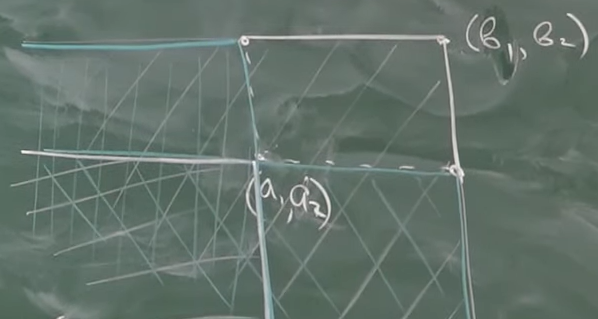
\includegraphics[width=10cm]{assets/02-general-prob-theory/arbitrary-value-independence.png}
            \end{center}

            $P_{\bar{\xi}}((a_1, b_1] \times (a_2, b_2]) = F_{\bar{\xi}} (b_1, b_2)  + F_{\bar{\xi}} (a_1, a_2) - F_{\bar{\xi}} (a_1, b_2) - F_{\bar{\xi}} (a_2, b_1) =$

            $= (F_{\xi_1} (b_1) - F_{\xi_1}(a_1)) \cdot (F_{\xi_2}(b_2) - F_{\xi_2}(a_2)) = P_{\xi_1} (a_1, b_1] \cdot P_{\xi_2}(a_2, b_2]$
        }
    \end{enumerate}
\end{proof}

\begin{consequence}
    $\xi_1 \ldots \xi_n$ - абсолютно непрерывные случайные величины. Тогда
    $\xi_1 \ldots \xi_n$ независимы $\Longleftrightarrow p_{\bar{\xi}} (\bar{t}) = p_{\xi_1} (t_1) \cdot \ldots \cdot p_{\xi_n}(t_n)$

    В частности, в случае независимости $\bar{\xi}$ абсолютно непрерывна.
\end{consequence}

\begin{proof}
    \begin{enumerate}
        \item {
            Докажем $\Rightarrow$.

            Независимость $\Rightarrow F_{\bar{\xi}} (\bar{x}) = F_{\xi_1} (x_1) \cdot \ldots \cdot F_{\xi_n} (x_n) =
            \int_{-\infty}^{x_1} p_{\xi_1} (t_1) \, dt_1 \cdot \ldots \cdot \int_{-\infty}^{x_n} p_{\xi_n} (t_n) \, dt_n =
            \int_{-\infty}^{x_1} \ldots \int_{-\infty}^{x_n} p_{\xi_1} (t_1) \ldots p_{\xi_n} (t_n) \, dt_n \ldots dt_1$.

            Запихали всё под один интеграл, то что под интегралом и есть совместная плотность.
        }
        \item {
            Докажем $\Leftarrow$.

            Просто проинтегрируем равенство.

            $\int_{-\infty}^{x_1} \ldots \int_{-\infty}^{x_n} p_{\bar{\xi}} (\bar{t}) \, dt_n \ldots dt_1 =
            \int_{-\infty}^{x_1} \ldots \int_{-\infty}^{x_n} p_{\xi_1} (t_1) \ldots p_{\xi_n} (t_n) \, dt_n \ldots dt_1 =$

            $\underbrace{=}_{\text{по т. Тонелли можно выносить интегралы}} F_{\xi_1} (x_1) \cdot \ldots \cdot F_{\xi_n} (x_n)$
        }
    \end{enumerate}
\end{proof}

\begin{remark}
    Напоминание.

    Свертка последовательностей: $\{a_n\}, \{b_n\}$ это $\{c_n\}$, такая что $c_n = a_0 b_n + a_1 b_{n - 1} + \ldots + a_n b_0$.

    Мотивировка: $\left(\sum_{n=0}^{\infty}a_n z^n\right) \cdot \left(\sum_{n = 0}^{\infty} b_n z^n\right) = \sum_{n=0}^{\infty} c_n z^n$  (при наличии хоть каких-нибудь кругов сходимости у обоих рядов).
\end{remark}

\begin{remark}
    \textbf{Свертки мер}

    $\mu$ и $\nu$ - конечные меры на борелевских подмножествах $\mathbb{R}$.

    $\mu * \nu (A) = \int_{\mathbb{R}} \mu (A - x) \, d\nu (x)$ - это свертка мер, где $(A - x) := \{ a - x \ | \ a \in A \}$.

    \begin{properties}
        \textbf{Свойства свёртки}

        \begin{enumerate}
            \item {
                $\mu * \nu (A) = \int_{\mathbb{R}^2} \mathds{1}_A (x + y) d\mu (x) \, d\nu (y)$

                \begin{proof}
                    $\mu * \nu (A) = \int_{\mathbb{R}} \mu (A - x) \, d\nu (x) \overset{\mu (A - x) = \int_{\mathbb{R}} \mathds{1}_{A - x} d\mu (y) }{=}
                    \int_{\mathbb{R}} \int_{\mathbb{R}} \mathds{1}_{A - x} (y) d\mu (y) \, d\nu (x)$
                \end{proof}
            }
            \item {
                $\mu * \nu = \nu * \mu$
            }
            \item {
                $\mu_1 * \ldots * \mu_n (A) = \int_{\mathbb{R}^n} \mathds{1}_A (x_1 + \ldots + x_n) \, d\mu_1 (x_1) \ldots \, d \mu_n (x_n)$
            }
            \item {
                $(\mu_1 * \mu_2) * \mu_3 = \mu_1 * (\mu_2 * \mu_3)$
            }
            \item {
                $(\mu_1 + \mu_2) * \nu = \mu_1 * \nu + \mu_2 * \nu$
            }
            \item {
                $\delta_x$ - мера с единичной нагрузкой в точке $x$. Тогда $\mu * \delta_0 = \mu$.

                Получили линейное пространство относительно $+$ и $*$

                \begin{proof}
                    $\mu * \delta_0 (A) = \delta_0 * \mu (A) = \int_{\mathbb{R}} \delta_0 (A - x) \, d\mu (x)
                    \overset{\delta_0 = 1 \Leftrightarrow 0 \in A - x \Leftrightarrow x \in A}{=} \int_{\mathbb{R}} \mathds{1}_{A} d\mu (x) = \mu A$
                \end{proof}
            }
        \end{enumerate}
    \end{properties}
\end{remark}

\begin{theorem}
    Пусть $\mu$ и $\nu$ имеют плотности $p_{\mu}$ и $p_{\nu}$

    Тогда $\mu * \nu$ имеет плотность $p(t) = \int_{\mathbb{R}} p_{\mu} (t - s) p_{\nu} (s) \, ds$
\end{theorem}

\begin{proof}
    Возьмём функцию, определяемую этой формулой и проверим, что подходит.

    $\int_A p(t) \, dt = \int_A \int_{\mathbb{R}} p_{\mu} (t - s) p_{\nu} (s) \, ds \, dt = \int_{\mathbb{R}}
    \int_{\mathbb{R}} \mathds{1}_A (t) p_{\mu} (t - s) p_{\nu} (s) \, ds \, dt = (*)$.

    Положим $u = t - s$. Тогда $(*) = \int_{\mathbb{R}^2} \mathds{1}_{A} (u + s) p_{\mu} (u) p_{\nu} (s) \, ds \, du =
    \int_{\mathbb{R}^2} \mathds{1}_A (u + s) \, d\nu (s) \, d \mu (u) = \mu * \nu (A)$
\end{proof}

\begin{theorem}
    Если $\xi$ и $\eta$ независимые случайный величины, то $P_{\xi + \eta} = P_{\xi} * P_{\eta}$
\end{theorem}

\begin{proof}
    Нужно взять какое-то борелевское множество и понять как устроено там распределение суммы.

    Пусть $B = \{ (x, y) : x + y \in A \}$

    $P_{\xi + \eta} (A) = P(\xi + \eta \in A) = P((\xi, \eta) \in B) = P_{\xi, \eta} (B) =
    \int_{\mathbb{R}^2} \mathds{1}_B (x, y) d P_{\xi} (x) \, dP_{\eta} (y) =
    \int_{\mathbb{R}^2} \mathds{1}_A (x + y) d P_{\xi} (x) \, dP_{\eta} (y) = P_{\xi} * P_{\eta} (A)$
\end{proof}

\begin{example}
    \begin{enumerate}
        \item {
            \textbf{Свертка с дисректным распределением}

            $\nu = \sum_{k = 1}^{\infty} p_k \delta_{x_k}$. Тогда $\mu * \nu (A) = \int_{\mathbb{R}} \mu (A - x) \, d\nu (x) =
            \sum_{k = 1}^{\infty} \mu (A - x_k) p_k$
        }
        \item {
            $\xi_i \sim Poisson(\lambda_i)$. $\xi_1$ и $\xi_2$ независимы.

            $P_{\xi_1 + \xi_2} (\{ n \}) = \sum_{k = 0}^{+\infty} P_{\xi_1} (\{ n  - k \}) \cdot
            \frac{\lambda_2^k e^{-\lambda_2}}{k!} = \sum_{k = 0}^{n} \frac{\lambda_1^{n - k} e^{-\lambda_1}}{(n - k)!} \cdot
            \frac{\lambda_2^k e^{-\lambda_2}}{k!} = e^{-\lambda_1} e^{-\lambda_2} \sum_{k = 0}^n \frac{\lambda_1^{n - k} \lambda_2^k}{k! (n - k)!} =
            \frac{(\lambda_1 + \lambda_2)^n e^{-\lambda_1 - \lambda_2}}{n!}$

            $\xi_1 + \xi_2 \sim Poisson(\lambda_1 + \lambda_2)$
        }
    \end{enumerate}
\end{example}



\Subsection{Математическое ожидание и дисперсия}

\begin{definition}
    $\xi : \Omega \rightarrow \mathbb{R}$ - случайная величина ($\xi \geq 0 $, либо суммируемая функция). $\mathbb{E} \xi = \int_{\mathbb{R}} \xi (\omega) \, dP(\omega)$ - математическое ожидание (среднее значение случайной величины).
\end{definition}

\begin{properties}
    \begin{enumerate}
        \item {
            $a, b \in \mathbb{R}: \ \mathbb{E} (a\xi + b \eta) = a\mathbb{E} \xi + b \mathbb{E} \eta$
        }
        \item {
            Если $\xi \geqslant 0$, с вероятностью 1, то $\mathbb{E} \xi \geqslant 0$ (по сути написано, что если функция почти везде неотрицательна, то интеграл неотрицателен).
        }
        \item {
            Если $\xi \geqslant \eta$ с вероятностью 1, то $\mathbb{E}\xi \geqslant \mathbb{E} \eta$
        }
        \item {
            $\mathbb{E} \xi = \int_{\mathbb{R}} x \, dP_{\xi} (x)$
        }
        \item {
            Если $f : \mathbb{R}^n \to \mathbb{R}$ - измерима относительно борелевской $\sigma-$алгебры.

            Тогда $\mathbb{E} f(\xi_1, \xi_2 \ldots \xi_n) = \int_{\mathbb{R}^n} f(x_1, \ldots, x_n) dP_{\xi_1, \ldots, \xi_n} (x_1, \ldots, x_n)$

            \textit{Доказательство:} $f = \mathds{1}_A$. Тогда $\mathbb{E} \mathds{1}_A (\xi_1, \ldots \xi_n) =
            \int_{\Omega} \mathds{1}_A (\xi_1 (w), \ldots, \xi_n (w)) dP(\omega) =
            P(\omega \in \Omega : \bar{\xi} \in A) = P_{\bar{\xi}} (A) = \int_{\mathbb{R}^n} \mathds{1}_A (x_1, \ldots, x_n) dP_{\bar{\xi}} (x_1, \ldots, x_n)$.

            Тогда по линейности верно для простых.

            Теперь берём $f_j$ неотрицательный простые, такие, что возрастают и $\rightarrow f$. И предельный
            переход по теореме Леви.
        }
        \item {
            Если $\xi_1$ и $\xi_2$ независимы, то $\mathbb{E} (\xi \cdot \eta) = \mathbb{E} \xi \cdot \mathbb{E} \eta$

            \textit{Доказательство: } $\mathbb{E} (\xi \eta) = \int_{\mathbb{R}^2} xy dP_{\xi, \eta} (x, y) = $

            $\underbrace{=}_{\text{независимость сл. вел.}} \int_{\mathbb{R}} \int_{\mathbb{R}} xy dP_{\xi} (x) \, dP_{\eta} (y) =
            \int_{\mathbb{R}} y \int_{\mathbb{R}} x dP_{\xi} (x) \, dP_{\eta} (y) = \mathbb{E} \xi \cdot \mathbb{E} \eta$
        }
        \item {
            Если $\xi \geqslant 0$, то $\mathbb{E} \xi = \int_{0}^{+\infty} P(\xi \geqslant t) \, dt$ - из теории меры.
        }
        \item {
            Если $p, q > 1$ и $\frac{1}{p} + \frac{1}{q} = 1$, то $\mathbb{E}|\xi \eta| \leqslant (\mathbb{E}|\xi|^p)^{\frac{1}{p}} (\mathbb{E} |\eta|^q)^{\frac{1}{q}}$ -
            неравенство Гёльдера
        }
        \item {
            Неравенство Ляпунова

            $0 < r < s$, тогда $(\mathbb{E} |\xi| ^ r)^{\frac{1}{r}} \leqslant (\mathbb{E}|\xi|^s)^{\frac{1}{s}}$.

            \textit{Доказательство:} $p = \frac{s}{r} > 1, \ \frac{1}{q} = 1 - \frac{1}{p} = \frac{s - r}{s} < 1$.

            Тогда запишем Гельдера для $\xi$ и $\eta = 1$:

            $\mathbb{E} |\xi|^r |1| \leq \left(\mathbb{E} (|\xi|^r)^p \right)^{\frac{1}{p}} \cdot \left( \mathbb{E} 1^q \right)^{\frac{1}{q}} = \left( \mathbb{E} |\xi|^s \right)^{\frac{r}{s}}$.

            % достаточно доказать для $r = 1$. То есть $\mathbb{E} |\xi| \leqslant (\mathbb{E}|\xi|^s)^{\frac{1}{s}}$.

            % Возьмём $\eta \equiv 1$ и напишем Гёльдера.
        }
    \end{enumerate}
\end{properties}

\begin{remark}
    $\mathbb{E}(\xi \eta) = \mathbb{E}\xi \cdot \mathbb{E} \eta$ без независимости неверно.

    Возьмём $\xi = \pm 1$ с вероятностями $\frac{1}{2}$. Тогда $\mathbb{E} \xi = 0$.

    Также пусть $\eta = \xi$. Тогда $\mathbb{\xi \eta} = \mathbb{E} \xi^2 = 1 \neq (\mathbb{E} \xi)^2$
\end{remark}

\begin{theorem}
    \textbf{Неравенство Маркова}

    Если $\xi \geqslant 0, p, t > 0$, то $P(\xi \geqslant t) \leqslant \frac{\mathbb{E}\xi^p}{t^p}$.
\end{theorem}

\begin{proof}
    Неравенство Чебышёва из теории меры.
\end{proof}

\begin{definition}
    \begin{enumerate}
        \item Моменты случайной величины. $\mathbb{E} (\xi^k)$ - $k$-ый момент.
        \item Центральный момент. $\mathbb{E}(\xi - \mathbb{E}\xi)^k$ - $k$-ый центральный момент.
        \item Абсолютный момент. $\mathbb{E}|\xi|^k$ - $k$-ый абсолютный момент.
    \end{enumerate}
\end{definition}

\begin{definition}
    Медиана случайной величины. $m$ - медиана $\xi$, если $P(\xi \geqslant m) \geqslant \frac{1}{2}$ и
    $P(\xi \leqslant m) \geqslant \frac{1}{2}$.

    \begin{remark}
        Медиана не единственна.

        Возьмём кубик. $\xi = 1, 2, \ldots, 6$ с вероятностью $\frac{1}{6}$.
        Тогда любое число $m \in [3, 4]$ подходит.

        Чаще всего всё равно берут середину, чтобы была единственность.
    \end{remark}
\end{definition}

\begin{example}
    Есть организация из 1000 человек. 1 начальник и 999 подчиненных.

    Зарплата начальника $1.000.000 \$ $, а подчинённых $1000 \$ $.

    $\mathbb{E} = \frac{999}{1000} \cdot 1000 + \frac{1}{1000} \cdot 1000000 = 1999$

    $m = 1000$ - медиана лучше характеризует ситуацию в этом случае.
\end{example}

\begin{definition}
    Дисперсия. $\mathbb{D} \xi = \mathbb{E}(\xi - \mathbb{E} \xi)^2$ - второй центральный момент.

    Обозначение в англоязычной литературе: $Var \xi$
\end{definition}

\begin{properties}
    \begin{enumerate}
        \item {
            $\mathbb{D} \xi = \mathbb{E} \xi^2 - (\mathbb{E} \xi)^2$

            \textit{Доказательство: } Пусть $a = \mathbb{E} \xi$.

            Тогда $\mathbb{D} \xi = \mathbb{E} (\xi - a)^2 = \mathbb{E} \xi^2 - 2a\mathbb{E}\xi + a^2$
        }
        \item {
            $\mathbb{D} \xi \geqslant 0$ и если $\mathbb{D} \xi = 0$, то $P(\xi = c) = 1$

            \textit{Доказательство: } Если $\mathbb{D} \xi = 0$, то
            $\int_{\Omega} (\xi - a)^2 \, dP = 0$, значит $(\xi - a)^2 = 0$ почти везде.
        }
        \item {
            $\mathbb{D} (\xi + a) = \mathbb{D} \xi$

            \textit{Доказательство: } $\mathbb{E} (\xi + a) = \mathbb{E} \xi + a$. А тогда
            $(\xi + a) - \mathbb{E} (\xi + a) = \xi - \mathbb{E} \xi$
        }
        \item {
            $\mathbb{D} (c \xi) = c^2 \mathbb{D} \xi$

            \textit{Доказательство: } $\mathbb{D} (c\xi) = \mathbb{E} (c\xi)^2 - (\mathbb{E} (c\xi))^2$
        }
        \item {
            Если $\xi$ и $\eta$ независимы, то $\mathbb{D} (\xi + \eta) = \mathbb{D}\xi + \mathbb{D} \eta$

            \textit{Доказательство: } $\mathbb{D} (\xi + \eta) = \mathbb{E} (\xi + \eta)^2 - (\mathbb{E} (\xi + \eta))^2 =
            \mathbb{E} \xi^2 + 2\mathbb{E}(\xi \eta) + \mathbb{E} \eta^2 - (\mathbb{E}\xi)^2 - 2\mathbb{E}\xi\mathbb{E}\eta - (\mathbb{E}\eta)^2 = \mathbb{D} \xi + \mathbb{D} \eta$
        }
        \item {
            Аналогично предыдущему, но для $n$ случайных величин.

            \textit{Доказательство: } индукция
        }
        \item {
            $\mathbb{E} |\xi - \mathbb{E} \xi| \leqslant \sqrt{\mathbb{D} \xi}$

            \textit{Доказательство: } $\mathbb{E} |\xi - \mathbb{E} \xi| \leqslant (\mathbb{E}|\xi - \mathbb{E}\xi|^2)^{\frac{1}{2}} = \sqrt{\mathbb{D} \xi}$ - написали Ляпунова.
        }
        \item {
            \textbf{Неравенство Чебышёва}

            $P(|\xi - \mathbb{E} \xi| \geqslant t) \leqslant \frac{\mathbb{D} \xi}{t^2}$, где $t > 0$

            \textit{Доказательство: } $P(|\xi - \mathbb{E} \xi| \geqslant t) \leqslant \frac{\mathbb{E} |\xi - \mathbb{E} \xi|^2}{t^2} = \frac{\mathbb{D}\xi}{t^2}$ - неравенство Маркова для $p = 2$.
        }
    \end{enumerate}
\end{properties}

\begin{definition}
    Стандартное отклонение $\sigma = \sqrt{\mathbb{D} \xi}$
\end{definition}

\begin{example}
    \begin{enumerate}
        \item {
            $\xi \sim U[0, 1]$.

            Тогда $\mathbb{E} \xi = \int_{0}^{1} x \, dx = \frac{x^2}{2} \bigg |_0^1 = \frac{1}{2}$.

            $\mathbb{E} \xi^2 = \int_{0}^{1} x^2 \, dx = \frac{x^3}{3} \bigg |_0^1 = \frac{1}{3}$. А тогда
            $\mathbb{D} \xi = \mathbb{E} \xi^2 - (\mathbb{E} \xi)^2 = \frac{1}{12}$
        }
        \item {
            $\xi \sim U[a, b]$.

            Если $\eta \sim U[0, 1]$ и $\xi = (b - a)\eta + a \sim U[a, b]$.
            Тогда $\mathbb{E} \xi = \mathbb{E} ((b - a) \eta  + a) = \frac{a + b}{2}$

            $\mathbb{D} ((b-a)\eta + a) = \mathbb{D} ((b - a)\eta) = (b-a)^2\mathbb{D}\eta = \frac{(b-a)^2}{12}$
        }
        \item {
            $\xi \sim \mathcal{N} (0, 1)$

            $\mathbb{E} \xi = \frac{1}{\sqrt{2\pi}} \int_{\mathbb{R}} xe^{\frac{-x^2}{2}} \, dx = 0$, так как функция нечётная.

            Значит $\mathbb{D} \xi = \mathbb{E} \xi ^2 = \frac{1}{\sqrt{2\pi}} \int_{\mathbb{R}} x^2 e^{-\frac{x^2}{2}} \, dx =
            -\frac{e^{\frac{-x^2}{2}}x}{\sqrt{2\pi}} \bigg |_{-\infty}^{+\infty} + \frac{1}{\sqrt{2\pi}} \int_{\mathbb{R}} e^{-\frac{x^2}{2}} \, dx = 1$
        }
        \item {
            $\xi \sim \mathcal{N}(a, \sigma^2)$

            Если $\eta \sim \mathcal{N}(0, 1)$, то $\xi = \sigma \eta + a \sim \mathcal{N}(a, \sigma^2)$.

            $\mathbb{E} \xi = \mathbb{E} (\sigma \eta + a) = \sigma \mathbb{E} \eta + a = a$

            $\mathbb{D} \xi = \mathbb{D} (\sigma \eta + a) = \sigma^2 \mathbb{D} \eta = \sigma^2$
        }
    \end{enumerate}
\end{example}

\begin{definition}
    Пусть $\mathbb{E} \xi^2 < +\infty$ и $\mathbb{E} \eta^2 < +\infty$.

    Ковариация $cov (\xi, \eta) = \mathbb{E} ((\xi - \mathbb{E}\xi)(\eta - \mathbb{E}\eta))$
\end{definition}

\begin{properties}
    \begin{enumerate}
        \item {
            $cov (\xi, \xi) = \mathbb{D} \xi$
        }
        \item {
            $cov (\xi, \eta) = cov (\eta, \xi)$
        }
        \item {
            $cov (c\xi, \eta) = c \cdot cov (\xi, \eta)$
        }
        \item {
            $cov(\xi_1 + \xi_2, \eta) = cov(\xi_1, \eta) + cov(\xi_2, \eta)$
        }
        \item {
            $cov (\xi, \eta) = \mathbb{E} (\xi \eta) - \mathbb{E}\xi\mathbb{E}\eta$

            \begin{proof}
                $\mathbb{E} \xi = a, \mathbb{E} \eta = b$

                $cov(\xi, \eta) = \mathbb{E}((\xi - a)(\eta - b)) = \mathbb{E}(\xi \eta) - a\mathbb{E}\eta - b \mathbb{E} \xi + ab$
            \end{proof}
        }
        \item {
            Если $\xi$ и $\eta$ независимы, то $cov (\xi, \eta) = 0$
        }
        \item {
            $\mathbb{D} (\xi + \eta) = \mathbb{D} \xi + \mathbb{D} \eta + 2 cov (\xi, \eta)$
        }
        \item {
            $\mathbb{D} (\xi_1 + \xi_2 + \ldots + \xi_n) = \mathbb{D} \xi_1 + \mathbb{D} \xi_2 + \ldots + \mathbb{E} \xi_n + 2\sum_{i < j} cov(\xi_i, \xi_j)$.
        }
    \end{enumerate}
\end{properties}

\begin{example}
    $P(\text{успех}) = p$. Делаем $n$ подбрасываний. $\eta =$ количество переходов от орла к решке.

    Пусть $\xi_i = 1$, если на $i$ позиции орёл, на $i + 1$ позиции решка, иначе $\xi_i = 0$.

    $\eta = \xi_1 + \ldots + \xi_{n - 1}$. Тогда $\mathbb{E} \eta = \sum_{i = 1}^{n - 1} \mathbb{E} \xi_i = (n - 1)pq$.

    $\mathbb{D} \eta = \sum_{i = 1}^{n - 1} \mathbb{D}\xi_i + 2\sum_{i < j} cov(\xi_i, \xi_j)$.

    Если $i + 1 < j$, то $\xi_i$ и $\xi_j$ независимы, поэтому в сумме почти везде нули.

    Значит $\mathbb{D} \eta = \sum_{i = 1}^{n - 1} \mathbb{D}\xi_i + 2\sum_{i = 1}^{n - 1} cov(\xi_i, \xi_{i + 1})$.

    $\mathbb{D} \xi_i = \mathbb{E} \xi_i^2 - (\mathbb{E} \xi_i)^2 = pq - p^2q^2$.

    $cov(\xi, \xi_{i + 1}) = \mathbb{E} (\xi_i \xi_{i + 1}) - \mathbb{E} \xi_i \mathbb{E} \xi_{i + 1} = -p^2q^2$
\end{example}

\begin{remark}
    \begin{enumerate}
        \item {
            $\{ \xi : \mathbb{E} \xi^2 < +\infty \}$

            $\left <\xi, \eta \right > = \mathbb{E} (\xi \eta)$ - скалярное произведение.

            $\mathbb{E} \xi$ - ортогональная проекция на константы.
        }
        \item {
            $\left < \xi, \eta \right > = cov (\xi, \eta)$ - тоже скалярное произведение.

            Норма - это стандартное отклонение.
        }
    \end{enumerate}
\end{remark}

\begin{theorem}
    \textbf{Выбор двудольного подграфа}

    Есть граф $G$ с $n$ вершинами и $m$ рёбрами. Хотим стереть некоторое количество рёбер(как можно меньше) так, чтобы
    остался двудольный подграф.

    Тогда $G$ содержит двудольный подграф с $\geqslant \frac{m}{2}$ рёбрами.
\end{theorem}

\begin{proof}
    $A$ - те вершины, на которых выпал орёл, $B$ - на которых выпала решка.

    Будем интересоваться матожиданием количества рёбер в такой ситуации. Пусть $xy \in E(G)$, сопоставим ребру
    следующую случайную величину:

    $
    \xi_{xy} =
    \begin{cases}
        1, & \text{если x, y из разных долей} \\
        0, & \text{иначе}
    \end{cases}
    $

    Пусть $\xi = \sum_{xy \in E} \xi_{xy}$ - число рёбер, которое нужно оставить, при таком разбиении на доли.

    $\mathbb{E} \xi = \sum_{xy \in E} \mathbb{E} \xi_{xy} = m \cdot (\frac{1}{2} \cdot 1 + \frac{1}{2} \cdot 0) = \frac{m}{2}$, а значит есть реализация с $\frac{m}{2}$ рёбрами.
\end{proof}

\begin{definition}
    Коэффициент корреляции. $\rho (\xi, \eta) = \frac{cov (\xi, \eta)}{\sqrt{\mathbb{D} \xi} \sqrt{\mathbb{D} \eta}} \in [-1, 1]$
\end{definition}

\begin{definition}
    Если $cov (\xi, \eta) = 0$, то это некоррелирующие случайные величины.
\end{definition}

\begin{theorem}

    $v_1, v_2 \ldots v_n \in \mathbb{R}^n$ - единичные векторы, тогда
    существует расстановка знаков $\varepsilon_1 = \pm 1, \ldots, \varepsilon_n = \pm 1$,
    такие, что $||\varepsilon_1 v_1 + \ldots + \varepsilon_nv_n|| \leqslant \sqrt{n}$.

    \begin{remark}
        Эта оценка не улучшаема, если все вектора попарно ортогональны, тогда
        длина вектора $\sqrt{n}$.
    \end{remark}
\end{theorem}

\begin{proof}
    Пусть $\varepsilon_1 \ldots \varepsilon_n$ - независимые случайные величины, такие, что:

    $
    \xi_{i} =
    \begin{cases}
        1, & \text{с вероятностью $\frac{1}{2}$} \\
        -1, & \text{с вероятностью $\frac{1}{2}$}
    \end{cases}
    $

    $\xi = || \varepsilon_1 v_1 + \ldots + \varepsilon_nv_n ||^2 $. И тогда $\mathbb{E} \xi = \mathbb{E} \left < v, v \right >  =
    \mathbb{E} (\sum_{i, j = 1}^n \varepsilon_i \varepsilon_j \left < v_i, v_j \right >) =
    \sum_{i, j = 1}^n \left < v_i, v_j \right > \mathbb{E} \varepsilon_i \varepsilon_j =
    \sum_{i = 1}^n \left < v_i, v_j \right > = n$.

    \begin{enumerate}
        \item Если $i = j$, то $\mathbb{E} \varepsilon_i \varepsilon_j = \mathbb{E} \varepsilon_i^2 = 1$
        \item Если $i \neq j$, то $\mathbb{E}\varepsilon_i \varepsilon_j \overset{\text{независимость}}{=} \mathbb{E} \varepsilon_i \cdot \mathbb{E} \varepsilon_j = 0$
    \end{enumerate}
\end{proof}

\begin{theorem}

    $v_1, v_2 \ldots v_n \in \mathbb{R}^n$, $|| v_i || \leqslant 1, p_i \in [0, 1] $ и
    $w = p_1v_1 + \ldots + p_n v_n$

    Тогда существует $\varepsilon_1 \in \{ 0, 1 \}, \ldots \varepsilon_n \in \{ 0, 1 \}$,
    такие, что $v = \varepsilon_1v_1 + \ldots + \varepsilon_nv_n$ и $|| v - w || \leqslant \frac{\sqrt{n}}{2}$
\end{theorem}

\begin{proof}
    Пусть $\varepsilon_1 \ldots \varepsilon_n$ - независимые случайные величины.

    $
    \varepsilon_{i} =
    \begin{cases}
        1, & \text{с вероятностью $p_i$} \\
        0, & \text{с вероятностью $1 - p_i$}
    \end{cases}
    $

    Интересуемся $\xi = || v - w ||^2$. Тогда $\mathbb{E} \xi = \mathbb{E} (\sum_{i, j = 1}^n (\varepsilon_i - p_i)(\varepsilon_j - p_j) \left < v_i, v_j \right > ) =
    \sum_{i, j = 1}^{n} \left < v_i, v_j \right > \mathbb{E} (\varepsilon_i - p_i)(\varepsilon_j - p_j) \overset{\text{пояснение ниже}}{=} \sum_{i = 1}^{n} \left < v_i, v_i \right > (p_i - p_i^2) \leqslant \frac{n}{4}$.

    \begin{enumerate}
        \item Если $i = j$, то $cov(\varepsilon_i, \varepsilon_j) = \mathbb{D}\varepsilon_i = p_i - p_i^2 \leqslant \frac{1}{4}$
        \item Если $i \neq j$, то $cov (\varepsilon_i, \varepsilon_j) \overset{\text{независимы}}{=} 0$
    \end{enumerate}
\end{proof}

\begin{example}
    $\Omega = \{ 1, 2 \ldots n \}$, пусть $\nu (k)$ - число различных простых В
    разложении $k$.

    \begin{theorem}
        \textbf{Харди-Рамануджана}

        Если $w(n) \to +\infty$, то $P(k \, : \, | \nu (k) - \ln \ln n| \geqslant w(n) \sqrt{\ln \ln n}) \to 0$
    \end{theorem}
\end{example}

\begin{proof}
    Пусть $m = \sqrt[10]{n}$. $p \leqslant m$ - простое и

    $
    \xi_p =
    \begin{cases}
        1, & \text{если $k$ делится на $p$} \\
        0, & \text{иначе}
    \end{cases}
    $

    $\xi = \sum_{p \leqslant m} \xi_p$ - количество различных простых $\leqslant m$. Тогда
    $\nu(k) - 10 \leqslant \xi (k) \leqslant \nu (k)$. Посчитаем матожидание $\xi$.

    $\mathbb{E} \xi_p = \frac{[\frac{n}{p}]}{n} \leqslant \frac{\frac{n}{p}}{n} = \frac{1}{p}$. С другой стороны,
    $\mathbb{E} \xi_p \geqslant \frac{\frac{n}{p} - 1}{n} = \frac{1}{p} - \frac{1}{n}$.

    Значит $\mathbb{E}\xi = \sum_{p \leqslant m} \mathbb{E}\xi_p. \sum_{p \leqslant m} \frac{1}{p} - \frac{m}{n} \leqslant
    \sum_{p \leqslant m} \mathbb{E}\xi_p \leqslant \sum_{p \leqslant m} \frac{1}{p} = \ln \ln m + \mathcal{O}(1) =
    \ln \ln n + \mathcal{O}(1)$. Оценка в другую сторону аналогично, потому что $\frac{m}{n} \leqslant 1$.

    Теперь считаем дисперсию.

    $\mathbb{D}\xi_p = \mathbb{E}\xi_p^2 - (\mathbb{E}\xi_p)^2 = \mathbb{E}\xi_p - (\mathbb{E}\xi_p)^2 \leqslant \frac{1}{p} - \frac{1}{p^2} + \frac{1}{n}$.
    С другой стороны $\mathbb{E}\xi_p^2 - (\mathbb{E}\xi_p)^2 \geqslant \frac{1}{p} - \frac{1}{n} - \frac{1}{p^2}$.

    $\sum_{p \leqslant m} \mathbb{D} \xi_p \sum_{p \leqslant m} \frac{1}{p} - \frac{1}{p^2} + \mathcal{O}(\frac{1}{n}) = \ln \ln n + \mathcal{O}(1)$.

    $cov(\xi_p, \xi_q) = \mathbb{E}\xi_p \xi_q = \mathbb{E} (\xi_p \xi_q) - \mathbb{E} \xi_p \mathbb{E}\xi_q$. Здесь
    $\frac{1}{pq} - \frac{1}{n} \leqslant \mathbb{E} \xi_p \xi_q \leqslant \frac{1}{pq}$. Тогда $cov(\xi_p, \xi_q) \leqslant
    \frac{1}{pq} - (\frac{1}{p} - \frac{1}{n})(\frac{1}{q} - \frac{1}{n}) = \frac{1}{n}(\frac{1}{p} + \frac{1}{q}) - \frac{1}{n^2} \leqslant \frac{1}{n}(\frac{1}{p} + \frac{1}{q})$.
    Также оцениваем в другую сторону.

    $-\frac{m^2}{n} = \mathcal{O}(1) \leqslant \sum_{p \neq q} cov (\xi_p, \xi_q) \leqslant \frac{1}{n}(\sum_{p \neq q} (\frac{1}{p} + \frac{1}{q})) =
    \frac{2m}{n} \sum_{p \leqslant m} \frac{1}{p} = \mathcal{O}(1)$.

    $\mathbb{D}\xi = \ln \ln n + \mathcal{O}(1)$. Теперь применим Чебышёва.

    $P(|\xi - \mathbb{E} \xi| \geqslant t) \leqslant \frac{\mathbb{D}\xi}{t^2}$. В качестве $t$ подставим $w(n) \sqrt{\ln \ln n}$.

    Тогда $P (|\nu - \ln \ln n| \geqslant w(n) \sqrt{\ln \ln n}) < P(|\xi - \mathbb{E} \xi| \geqslant w(n) \sqrt{\ln \ln n}) \leqslant \frac{\mathbb{D}\xi}{w^2(n) \ln \ln n} \to 0$.

\end{proof}

\begin{remark}
    \begin{theorem}
        \textbf{Эрдёша-Каца}

        $P(k \in \Omega \, : \, a \leqslant \frac{|\nu (k) - \ln \ln n|}{\sqrt{\ln \ln n}} \leqslant b ) \rightarrow \frac{1}{\sqrt{2\pi}} \int_{a}^{b} e^{-\frac{t^2}{2}} \, dt $
    \end{theorem}
\end{remark}

\Subsection{Сходимость последовательностей случайных величин}

\begin{theorem}
    $\xi_1, \xi_2, \ldots$ - независимые случайные величины, $f_i : \mathbb{R}^{n_i} \to \mathbb{R}$ - измерима,
    относительно борелевской $\sigma$-алгребры.

    Тогда $f_1 (\xi_1, \ldots \xi_{n_1}), f_2(\xi_{n_1 + 1}, \ldots, \xi_{n_1 + n_2})$ - независимые случаные величины.
\end{theorem}

\begin{proof}
    $f : \mathbb{R}^m \to \mathbb{R}$ и $g : \mathbb{R}^n \to \mathbb{R}$. $f(\xi_1 \ldots \xi_m)$ и
    $g(\eta_1 \ldotp \eta_n)$ независимые.

    Возьмём $\tilde{A}$ и $\tilde{B} \in \mathbb{R}$ борелевские. Надо доказать, что
    $P(f(\xi_1 \ldots \xi_m) \in \tilde{A}) \cdot P(g(\eta_1 \ldots \eta_n) \in \tilde{B}) =
    P(f(\xi_1, \ldots, \xi_m) \in \tilde{A}, g(\eta_1 \ldotp \eta_n) \in \tilde{B})$.

    $P((\xi_1, \ldots, \xi_m) \in f^{-1} (\tilde{A}) = A) \cdot P((\eta_1, \ldots, \eta_m) \in f^{-1} (\tilde{B}) = B) = P(\ldots)$

    Поймём это для ячеек.

    $A = (a, b]$, что такое $P((\xi_1, \ldots, \xi_m) \in (a, b]) = P(\xi_1 \in (a_1, b_1], \ldots, \xi_m \in (a_m, b_m]) = P(\ldots) \cdot \ldots \cdot P(\ldots)$.

    Если $A_j$ дизъюнктны $P((\xi_1, \ldots, \xi_m) \in A_j) \cdot P((\eta_1, \ldots, \eta_m) \in B) = P(\ldots).$
    Просуммируем $P((\xi_1, \ldots, \xi_m) \in \bigsqcup A_j) \cdot P((\eta_1, \ldots, \eta_m) \in B) = P(\ldots)$
\end{proof}

\begin{definition}
    $\xi, \xi_1, \xi_2, \ldots : \Omega \to \mathbb{R}$.

    \begin{enumerate}
        \item $\xi_n$ сходится к $\xi$ почти наверное, если $P(w \in \Omega : \lim_{n \to \infty} \xi_n(w) = \xi (w)) = 1$
        \item $\xi_n$ сходится к $\xi$ в среднем порядка $r > 0$, если $\mathbb{E} (|\xi_n - \xi|^r) \rightarrow_{n \to \infty} 0$
        \item $\xi_n$ сходится к $\xi$ по вероятности, если $\forall \varepsilon > 0,  \, P(|\xi_n - \xi| \geqslant \varepsilon) \rightarrow_{n \to \infty} 0$
        \item $\xi_n : \Omega_n \to \mathbb{R}$. $\xi_n$ сходится к $\xi$ по распределению, если
        $\lim_{n \to \infty} F_{\xi_n} (x) = F_{\xi} (x)$ во всех точках непрерывности $F_{\xi}$
    \end{enumerate}

    Связь между ними $1 \Rightarrow 3, 2 \Rightarrow 3$ (неравенство Маркова). При этом $3 \not \Rightarrow 1, 2 \not \Rightarrow 1$
    \color{red}
      TODO
    \color{black}
    %TODO
    %TODO

    $4 \not \Rightarrow 3$. Да и вообще они на разных вероятностных пространствах,
    так что постановка вопроса в целом неверная.

    $3 \Rightarrow 4$. $\{ \xi_n > x \} \supset \{ \xi > x+ \varepsilon \} \cap \{ |\xi_n - \xi| < \varepsilon \}$. Также верно обратное:
    $\{ \xi_n \leqslant x \} \subset \{ \xi \leqslant x+ \varepsilon \} \cup \{ |\xi_n - \xi| \geqslant \varepsilon \}$.

    Тогда $F_{\xi_n}(x) \leqslant F_{\xi}(x + \varepsilon) + P(|\xi_n - \xi| \geqslant \varepsilon)$.
    $\bar{\lim} F_{\xi_n}(x) \leqslant F_{\xi}(x + \varepsilon) + \bar{\lim} P(|\xi_n - \xi| \geqslant \varepsilon) = F_{\xi}(x + \varepsilon)$.

    $\{ \xi_n > x \} \subset \{ \xi > x - \varepsilon \} \cup \{ |\xi_n - \xi| \geqslant \varepsilon \}$ - запишем через вероятности.
    $1 - F_{\xi_n}(x) \leqslant 1 - F_{\xi}(x - \varepsilon) + P(|\xi_n - \xi| \geqslant \varepsilon)$. То есть
    $\underline{\lim} F_{\xi_n}(x) \geqslant F_{\xi}(x - \varepsilon) - \lim P(|\xi_n - \xi| \geqslant \varepsilon) = F_{\xi}(x - \varepsilon)$.

    То есть $F_{\xi}(x - \varepsilon) \leqslant \underline{\lim} F_{\xi_n}(x) \leqslant \overline{\lim} F_{\xi_n}(x) \leqslant F_{\xi}(x + \varepsilon)$ - верно для любого $n$.
    Устремим $\varepsilon \rightarrow 0$. Тогда $F_{\xi}(x) \leqslant \underline{\lim} F_{\xi_n}(x) \leqslant \overline{\lim} F_{\xi_n}(x) \leqslant F_{\xi}(x)$, но левая и правая штука равны.

\end{definition}

\begin{theorem}
    \textbf{Закон больших чисел}

    $\xi_1, \xi_2, \ldots$ - попарно некоррелируемые случайные величины и
    $\mathbb{D}\xi_n = o(n)$.

    $S_n = \xi_1 + \xi_2 + \ldots + \xi_n$.

    Тогда $\frac{S_n}{n} - \mathbb{E}\frac{S_n}{n} \underset{P}{\rightarrow} 0$.
    То есть вероятность того, что $P(|\frac{S_n}{n} - \mathbb{E}\frac{S_n}{n}| \geqslant \varepsilon) \rightarrow 0$
\end{theorem}

\begin{consequence}
    Если $\mathbb{D}\xi_n$ ограничены, то такой же вывод.
\end{consequence}

\begin{proof}
    $P(\left |\frac{S_n}{n} - \mathbb{E}\frac{S_n}{n} \right | \geqslant \varepsilon) \leqslant \frac{\mathbb{D}\frac{S_n}{n}}{\varepsilon^2} = \frac{\mathbb{D}S_n}{\varepsilon^2n^2} =
    \frac{\sum_{k = 1}^n \mathbb{D}\xi_k}{\varepsilon^2n^2} \rightarrow_{\text{Штольц}} \lim_{n \to \infty} \frac{\mathbb{D}\xi_n}{\varepsilon^2(2n - 1)} = 0$.
\end{proof}

\begin{consequence}
    \textbf{ЗБЧ в форме Чебышёва}

    $\xi_1, \xi_2, \ldots$ независимые, одинаково распределенённые случайные величины с конечной дисперсией.
    Пусть $a = \mathbb{E}_{\xi_1}$

    Тогда $P(\left | \frac{S_n}{n} - a \right | \geqslant \varepsilon) \rightarrow 0$ или же $\frac{S_n}{n} \underset{P}{\rightarrow} a$

    \begin{proof}
        Мат. ожидание всех случайных величин равно, они одинаково распределены. Поэтому
        $\mathbb{E} \frac{S_n}{n} = \mathbb{E} \frac{\xi_1 + \ldots + \xi_n}{n} = a$. Поэтому все условия предыдущей
        теоремы выполнены
    \end{proof}
\end{consequence}

\begin{consequence}
    \textbf{ЗБЧ для схем Бернулли}

    Есть схема Бернулли с вероятностью успеха $p$.

    Тогда $\frac{S_n}{n} \underset{P}{\rightarrow} p$
\end{consequence}

\begin{theorem}
    \textbf{Усиленный ЗБЧ}

    $\xi_1, \xi_2, \ldots$ - независимые случайные величины.
    $\mathbb{E} (\xi_n - \mathbb{E}\xi_n)^4 \leqslant C$.

    Тогда $\frac{S_n}{n} - \mathbb{E} \frac{S_n}{n} \rightarrow 0$ почти наверное.
\end{theorem}

\begin{proof}
    $\frac{S_n}{n} - \mathbb{E}\frac{S_n}{n} = \frac{1}{n} (S_n - \mathbb{E}S_n) = \frac{1}{n}(\sum_{k = 1}^n (\xi_k - \mathbb{E}\xi_k))$. Задвинем все
    матожидания в ноль.

    Тогда по условию $\mathbb{E} \xi_n^4 \leqslant C$ и надо доказать, что $\frac{S_n}{n} \rightarrow 0$ почти наверное.

    Пусть $A_n = \{ \left | \frac{S_n}{n} \right | \geqslant \varepsilon \}$. Нам нужно понять, что бесконечное количество $A_n$ случаются
    с нулевой вероятностью.

    Из леммы Бореля-Кантелли, если $\sum_{k = 1}^{\infty} \sum_{k = 1}^{\infty} P(A_n) < +\infty$, то нужное нам условие выполнено.

    Напишем неравенство Маркова: $P(A_n) \leqslant \frac{\mathbb{E} \frac{S_n^4}{n^4}}{\varepsilon^4} = \frac{\mathbb{E}S_n^4}{n^4\varepsilon^4}$. Достаточно доказать, что
    $\mathbb{E}S_n^4 = \mathcal{O}(n^2)$, тогда ряд сойдётся. Раскроем все скобки.

    $\mathbb{E}(\xi_1 + \ldots + \xi_n)^4 = \sum_{i = 1}^n \mathbb{E}\xi_i^4 + 4\sum_{i \neq j}\mathbb{E}\xi_i^3\xi_j +
     6\sum_{i \neq j}\mathbb{E}\xi_i^2 \xi_j^2 + 12\sum_{i \neq j \neq k} \mathbb{E} \xi_i^2 \xi_j \xi_k + 24\sum_{\ldots} \mathbb{E}\xi_i \xi_j \xi_k \xi_m$

    \begin{enumerate}
        \item {
            $\mathbb{E}\xi_i \xi_j \xi_k \xi_m = 0$
        }
        \item {
            $\mathbb{E} \xi_i^2 \xi_j \xi_k = 0$
        }
    \end{enumerate}

    Итого получаем $\sum_{i = 1}^n \mathbb{E}\xi_i^4 + 6 \sum \mathbb{E}x_i^2 \mathbb{E}\xi_j^2$ (*). По неравенству Ляпунова
    $\mathbb{E}\xi_i^2 \leqslant \sqrt{\mathbb{E}\xi_i^4} \leqslant \sqrt{C}$.

    Значит $(*) = nC + 6n(n-1)\sqrt{C}\sqrt{C} \leqslant 6Cn^2 = \mathcal{O}(n^2)$, значит ряд сходится и лемма Бореля-Кантелли выполняется.
\end{proof}

\begin{consequence}
    \textbf{Усиленный ЗБЧ для схем Бернулли}

    В схеме Бернулли с вероятностью успеха $p \, : \, \frac{S_n}{n} \rightarrow p$ почти наверное.
\end{consequence}

\begin{proof}
    Нужно проверить, что $\mathbb{E}(\xi_i - p)^4$ - конечно, раскроем скобки, получим какие-то константы и $\xi_i^p$.
\end{proof}

\begin{theorem}
    \textbf{Усиленный ЗБС в форме Колмогорова}

    $\xi_1, \xi_2, \ldots$ - независимо, одинаково распределённые случайные величины.

    Тогда $\frac{S_n}{n} \rightarrow a \in \mathbb{R}$ почти наверное $\Leftrightarrow a = \mathbb{E}\xi_1$
\end{theorem}


\textbf{Метод Монте-Карло}

$\Phi$ - ограниченная фигура на плоскости. Хотим примерно узнать её площадь.

Берём случайную точку в прямоугольнике и выясняем, попала она в фигуру или нет.

$
\xi_i =
\begin{cases}
    1, & \text{точка попала в $\Phi$} \\
    0, & \text{иначе}
\end{cases}
$

Вероятность успеха $\frac{Area(\Phi)}{Area(\text{прямоугольника})}$. Тогда усиленный ЗБЧ
говорит, что $\frac{S_n}{n} \rightarrow p$ почти наверное.

\begin{theorem}
    $\xi_1, \xi_2, \ldots$ последовательность случайных величин, $\xi_n \rightarrow_P a \in \mathbb{R}$.
    $f$ ограниченная функция, непрерывная в точке $a$.

    Тогда $\mathbb{E}f(\xi_n) \rightarrow f(a)$
\end{theorem}

\begin{proof}
    $|\mathbb{E} f(\xi_n) - f(a)| = |\mathbb{E} (f(\xi_n) - f(a))| \leqslant \mathbb{E} |f(\xi_n) - f(a)| =
    \mathbb{E} |f(\xi_n - f(a))|\cdot \mathds{1}_{\{ \xi_n - a < \varepsilon \}} + \mathbb{E} |f(\xi_n - f(a))|\cdot \mathds{1}_{\{ \xi_n - a \geqslant \varepsilon \}} = (*)$.

    Пусть $f$ ограничена константой $M$.

    $\mathbb{E} |f(\xi_n - f(a))|\cdot \mathds{1}_{\{ \xi_n - a \geqslant \varepsilon \}} \leqslant 2M \mathbb{E} \mathds{1}_{\{ \xi_n - a \geqslant \varepsilon \}}$

    $|f(\xi_n - f(a))|\cdot \mathds{1}_{\{ \xi_n - a < \varepsilon \}} \leqslant \sup_{|x - a| < \varepsilon}|f(x) - f(a)|$

    Тогда $(*) \leqslant \sup_{|x - a| < \varepsilon} |f(x) - f(a)| + 2M P(|\xi_n - a| \geqslant \varepsilon)$.

    $\overline{\lim} |\mathbb{E} f(\xi_n) - f(a)| \leqslant \sup_{|x - a| < \varepsilon} |f(x) - f(a)| + 2M \overline{\lim} P(|\xi_n - a| \geqslant \varepsilon) \leqslant
    \sup_{|x - a| < \varepsilon} |f(x) - f(a)| \rightarrow 0$ при $\varepsilon \to 0$.

    Тогда $0 \leqslant \underline{\lim} \leqslant \overline{\lim} \leqslant 0 \Rightarrow \lim |\mathbb{E} f(\xi_n) - f(a)| = 0$
\end{proof}

\begin{remark}
    В условии теоремы $|\mathbb{E} f(\xi_n) - f(a)| \leqslant \sup_{|x - a| < \varepsilon} |f(x) - f(a)| + 2M P(|\xi_n - a| \geqslant \varepsilon)$
\end{remark}

\begin{theorem}
    \textbf{Вейерштрасса}

    $f \in C[a, b]$, то существует последовательность многочленов $P_n$, такая, что $P_n \rightrightarrows f$ на $[a, b]$
\end{theorem}

\begin{proof}
    Можно считать, что всё на $[0, 1]$. Рассмотрим схему Бернулли с вероятностью успеха $p$.
    Тогда $\frac{S_n}{n} \rightarrow p$. Подставим $\xi_n = \frac{S_n}{n}$ в замечание.

    $|\mathbb{E} f(\frac{S_n}{n}) - f(p)| \leqslant \sup_{|x - a| < \varepsilon} |f(x) - f(a)| + 2M P(|\frac{S_n}{n} - p| \geqslant \varepsilon) = (*)$

    Из неравенства Чебышёва $P(|\frac{S_n}{n} - p| \geqslant \varepsilon) \leqslant \frac{\mathbb{D}\frac{S_n}{n}}{\varepsilon^2} = \frac{np(1 - p)}{n^2\varepsilon^2} \leqslant \frac{1}{4n\varepsilon^2}$.

    И тогда $(*) \leqslant \sup_{|x - y| < \varepsilon} |f(x) - f(y)| + \frac{M}{2n\varepsilon^2}$. При $n = \frac{1}{\varepsilon^3}$ правое слагаемое оценивается $\varepsilon'$, а первое
    слагаемое мало из равномерной непрерывности.

    Значит $\mathbb{E} f(\frac{S_n}{}n) - f(p) \rightrightarrows 0$. $\mathbb{E} f(\frac{S_n}{n}) = \sum_{k = 0}^n f(\frac{k}{n}) \cdot \binom{n}{k} p^k (1 - p)^{n - k}$ - многочлен Бернштейна.
\end{proof}

\begin{definition}
    Многочлен Бернштейна $B_n(x) = \sum_{k = 0}^n f(\frac{k}{n}) \binom{n}{k} x^k (1-x)^{n - k}$
\end{definition}

\begin{consequence}
    \begin{enumerate}
        \item {
            $B_n(0) = f(0)$
        }
        \item {
            $B_n(1) = f(1)$
        }
        \item {
            $B_n'(0) = n(f(\frac{1}{n}) - f(0))$

            $B_n'(1) = n(f(1) - f(\frac{n - 1}{n}))$

            \textit{Доказательство: } $B_n'(x) = \sum_{k = 0}^n f(\frac{k}{n})\binom{n}{k} (kx^{k - 1}(1 - x)^{n - k} - (n - k)x^k(1-x)^{n - k - 1}) = $

            $= \sum_{k = 0}^n f(\frac{k}{n}) \binom{n}{k} x^{k-1}(1-x)^{n - k - 1}(k - nx)$
        }
        \item {
            $B_n'(x) = \sum_{k = 0}^n f(\frac{k}{n}) f(\frac{k}{n}) \binom{n}{k} x^{k-1}(1-x)^{n - k -1} (k - nx)$
        }
        \item {
            $B_n(\alpha f + \beta g, x) = \alpha B_n(f, x) + \beta B_n(g, x)$
        }
    \end{enumerate}
\end{consequence}

\textbf{Кривые Безье}

$\sum_{k = 0}^n a_k \binom{n}{k} t^k (1 - t)^{n - k}, a_k \in \mathbb{R}^2$. Получается
отображение $\gamma \, : \, [0, 1] \to \mathbb{R}^2$.

\begin{enumerate}
    \item {
        $n = 1 \, : \, a(1 - t) + bt$ - отрезок соединяющий точки $a$ и $b$.
    }
    \item {
        $n = 2 \, : \, a(1 - t)^2 + 2bt(1 - t) + ct^2$. Мы знаем, что $B'(0) = 2(b - a)$ и $B'(1) = 2(c - b)$.
        Это кривая из точки $a$ в $c$, параметр $b$ задаёт касательную в $a$ и $c$.
    }
    \item {
        $n = 3 \, : \, a(1 - t)^3 + 3bt(1-t)^2 + 3ct^2(1 - t) + dt^3$.

        Здесь $B(0) = a, B(1) = d, B'(0) = 3(b - a), B'(1) = 3(d - c)$. Кривая выходит
        из точки $a$ с касательной $3(b - a)$, а заходит в точку $d$ с касательной $3(d - c)$.
    }
\end{enumerate}

\Subsection{Производящие функции}

\begin{definition}
    $\xi : \Omega \to \{ 1, 2, \ldots \}$ - случайная величина.

    $G_{\xi} (z) = \sum_{n=0}^{\infty} P(\xi = n)z^n$ - производящая фукнция
\end{definition}

\begin{properties}
    \begin{enumerate}
        \item {
            $G_{\xi}$ однозначно определяет распределение
        }
        \item {
            $G_{\xi}(1) = 1$ и $G_{\xi}$ сходится в круге $|z| < 1$.
        }
        \item {
            $G_{\xi} (x) = \mathbb{E} x^{\xi}$, где $x \in \mathbb{R}$

            \textit{Доказательство: } $\mathbb{E} x^{\xi} = \sum_{n=0}^{\infty} x^{n} \cdot P(\xi = n) = G_{\xi} (x)$
        }
        \item {
            $G_{\xi}'(1) = \mathbb{E} \xi$

            \textit{Доказательство: } $G_{\xi}'(x) = \sum_{n = 1}^{\infty} P(\xi = n) nx^{n-1}$ - если подставить единицу - получим матожидание.
        }
        \item {
            $\mathbb{E}\xi^2 = G_{\xi}''(1) + G_{\xi}'(1)$

            \textit{Доказательство: } $G_{\xi}''(x) = \sum_{n = 2}^{\infty} P(\xi = n) n(n-1)x^{n-2}$ - если подставить единицу - получим матожидание.
        }
        \item {
            $\mathbb{D} \xi = \mathbb{E}\xi^2 - (\mathbb{E}\xi)^2  = G_{\xi}''(1) + G_{\xi}'(1) - (G_{\xi}'(1))^2$
        }
        \item {
            $G_{\xi}$ возрастает и выпукла на $[0, 1]$
        }
        \item {
            Если $\xi$ и $\eta$ независимы, то $G_{\xi + \eta}(z) = G_{\xi}(z) \cdot G_{\eta}(z)$

            \textit{Доказательство: } $x^\xi$ и $x^\eta$ независимы, а тогда $\mathbb{E} (x^\xi \cdot x^\eta) = \mathbb{E} x^{\xi} \cdot \mathbb{E} x^{\eta}$
        }
    \end{enumerate}
\end{properties}

\begin{example}
    \begin{enumerate}
        \item {
            Равномерное распределение на $\{ 0, 1, \ldots, n - 1 \}$.

            Тогда $G_{\xi}(z) = \frac{1}{n}(1 + z + z^2 + \ldots z^{n - 1}) = \frac{1 - z^n}{1 - z} \cdot \frac{1}{n}$. Пусть хотим
            посчитать матожидание и диспресию, но единицу то подставить нельзя в свернутую формулу. Решается эта проблема так:

            Давайте скажем, что $z = 1 + y$. Тогда $G_{\xi}(1 + y) = \frac{(1 + y)^n - 1}{ny} = 1 + \binom{n}{2} \frac{y}{n} + \binom{n}{3} \frac{y^2}{n} \ldots$

            Тогда $G_{\xi}'(1) = \frac{\binom{n}{2}}{n} = \frac{n - 1}{2}$, $\mathbb{E} \xi^2 = G_{\xi}''(1) + G_{\xi}'(1) = 2\frac{n(n-1)(n-2)}{6n} + \frac{n - 1}{2} =
            \frac{n - 1}{2}(\frac{2n - 4}{3} + 1) = \frac{n - 1}{2} \cdot \frac{2n - 1}{3}$. И тогда $\mathbb{D} \xi = \mathbb{E}\xi^2 - (\mathbb{E}\xi)^2 =
            \frac{n - 1}{2} \cdot \frac{n + 1}{6} = \frac{n^2 - 1}{12}$
        }
        \item {
            \textbf{Задача Галилея}

            Есть 3 правильных кубика, бросили и посчитали сумму значений. Интересуемся вероятностью того, что
            в сумме выпало 10.

            $P(\text{в сумме 10}) = ?$

            $\xi_i$ - значение на $i$-том кубике. Тогда $G_{\xi_i}(z) = \frac{1}{6}(z + z^2 + \ldots + z^6) = \frac{z(1 - z^6)}{1 - z} \cdot \frac{1}{6}$.
            Кубика у нас три, поэтому нас интересует $G_{\xi_1 + \xi_2 + \xi_3} = G_{\xi_1} \cdot G_{\xi_2} \cdot G_{\xi_3} = \left ( \frac{z(1 - z^6)}{1 - z} \cdot \frac{1}{6} \right )^3 = (*)$

            $\frac{1}{(1 - z)^3} = \sum_{n = 0}^{\infty} \binom{n+2}{n} z^n$. Тогда $(*) = \frac{1}{6^3} (z^3 - 3z^9 + 3z^15 - z^21) \cdot \sum_{n = 0}^{\infty} \binom{n+2}{n} z^n$. Коэффициент при $z^{10}$ будет такой
            $\frac{1}{6^3} (1 \cdot \binom{9}{7} - 3 \cdot \binom{3}{1}) = \frac{1}{6^3} (36 - 3^2) = \frac{1}{8}$
        }
    \end{enumerate}
\end{example}
\Section{Метод характеристических функций}{Виноградов Александр}
\Subsection{Характеристические функции случайных величин}

\begin{definition}
    Комплекснозначная случайная величина $\xi = \Re \xi + i \Im \xi$, где $\Re \xi$ и $\Im \xi$
    вещественнозначные случайные величины.
\end{definition}

\begin{definition}
    $\xi : \Omega \to \mathbb{C}$

    $\mathbb{E} \xi = \mathbb{E} \Re \xi + i \mathbb{E} \Im \xi$
\end{definition}

\begin{properties}
    \begin{enumerate}
        \item {
            $\mathbb{E} (i \xi) = i \mathbb{E}\xi$
        }
        \item {
            Комплексная линейность $\mathbb{E} (\alpha \xi + \beta \eta) = \alpha \mathbb{E} \xi + \beta \mathbb{E} \eta$, где $\alpha, \beta \in \mathbb{C}, \xi, \eta : \Omega \to \mathbb{C}$

            \textit{Доказательство: } $\mathbb{E} (\alpha \xi) = \mathbb{E} (a + ib)\xi = \mathbb{E} (a \xi) + \mathbb{E} (b\xi i) = (a + bi) \mathbb{E} \xi$
        }
        \item {
            $\overline{\mathbb{E} \xi} = \mathbb{E} \overline{\xi}$
        }
        \item {
            $|\mathbb{E} \xi | \leqslant \mathbb{E} |\xi|$

            \textit{Доказательство: } Возьмём $c \in \mathbb{C}, |c| = 1$, такой, что $\mathbb{E} (c \xi) = |\mathbb{E} \xi|$, то есть $c = \frac{|\mathbb{E} \xi|}{\overline{\mathbb{E} \xi}}$ (или $c = e^{-i \cdot \arg \mathbb{E}\xi}$).

            Тогда $|\mathbb{E} \xi| = \mathbb{E} (c \xi) = \mathbb{E} (\Re (c \xi)) \leqslant \mathbb{E} |\Re (c \xi)| \leqslant \mathbb{E} |c \xi | = \mathbb{E} |\xi|$
        }
    \end{enumerate}
\end{properties}

\begin{definition}
    Ковариация $cov(\xi, \eta) = \mathbb{E} (\xi - \mathbb{E}\xi)\overline{(\eta - \mathbb{E} \eta)}$
\end{definition}

\begin{definition}
    Дисперсия $\mathbb{D} \xi = \mathbb{E} |\xi - \mathbb{E}\xi|^2$

    $cov(\xi, \xi) = \mathbb{D}\xi$
\end{definition}

\begin{definition}
    $\xi : \Omega \to \mathbb{R}$. Назовём характеристической функцией $\xi$:

    $\phi_\xi (t) = \mathbb{E} e^{it\xi}$, где $t \in \mathbb{R}$
\end{definition}

\begin{properties}
    \begin{enumerate}
        \item {
            $\phi_\xi (0) = 1$ и $|\phi_\xi (t)| \leqslant 1$

            \textit{Доказательство: } $|\phi_\xi (t)| \leqslant |\mathbb{E} e^{it\xi}| \leqslant \mathbb{E}|e^{it\xi}| = 1$
        }
        \item {
            $\phi_{a\xi + b} (t) = e^{ibt} \phi_\xi (at)$

            \textit{Доказательство: } $\phi_{a\xi + b} (t) = \mathbb{E} e^{i(a \xi + b)t} = \mathbb{E} e^{ibt} e^{i\xi a t} = e^{ibt} \mathbb{E} e^{i\xi (at)} = \phi_{\xi} (at) e^{ibt} $
        }
        \item {
            Если $\xi$ и $\eta$ независимы, то $\phi_{\xi + \eta} (t) = \phi_\xi (t) \cdot \phi_{\eta} (t)$

            \textit{Доказательство: } $e^{i\xi t}$ и $e^{i \eta t}$ независимы и пишем произведение матожиданий
        }
        \item {
            $\overline{\phi_{\xi}(t)} = \phi_{\xi} (-t)$

            \textit{Доказательство: } $\overline{\phi_{\xi}(t)} = \overline{\mathbb{E} e^{i \xi t}} = \mathbb{E} \overline{e^{i \xi t}} = \mathbb{E} e^{-i \xi t} = \phi_\xi (-t)$
        }
        \item {
            $\phi_{\xi}$ равномерно непрерывна на $\mathbb{R}$

            \textit{Доказательство: } $|\phi_{\xi}(t + h) - \phi_{\xi}(t)| = | \mathbb{E} e^{i (t + h) \xi} - \mathbb{E} e^{i t \xi} | = | \mathbb{E} \left( e^{it \xi} (e^{i h \xi} - 1) \right) | \leq $

            $\leq \mathbb{E} \left| e^{it \xi} (e^{i h \xi} - 1) \right| = \mathbb{E} | e^{i h \xi} - 1 | = \int_{\mathbb{R}} | e^{i h x} - 1 | d P_{\xi}(x) \rightarrow_{(*)} 0$.

            $(*)$: Знаем, что $e^{i h x} \rightarrow_{h \to 0} 1$, хотим понять, что можно вносить предел под знак интеграла. Это сделать можно по теорема Лебега, где суммируемая мажоранта будет $2$, так как мера вероятностная.

            \textbf{Напоминание Th Лебега:}\newline

            \begin{center}
                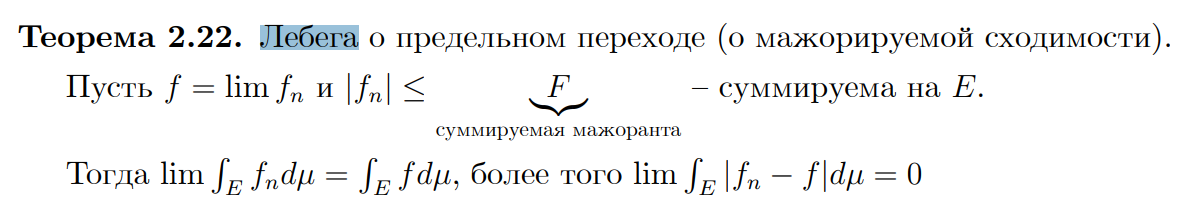
\includegraphics[scale=0.7]{./assets/03-characteristic-funcs/lebegs-theorem.PNG}
            \end{center}

            %$|\phi_{\xi} (t + h) - \phi_{\xi}(t)| = |\mathbb{E} (e^{i \xi (t + h) - \mathbb{E} e^{i \xi t}}) | = |\mathbb{E} (e^{i\xi t} \cdot e^{i \xi h}) - \mathbb{E} e^{i \xi t}| =
            %|\mathbb{E} (e^{i \xi t}(e^{i \xi h} - 1))| \leqslant \mathbb{E} |e^{i \xi t}| \cdot |e^{i \xi h} - 1| $

            %$\lim_{h \to 0} \int_{\Omega} |e^{}|$
        }
    \end{enumerate}
\end{properties}

\begin{example}
    $\xi \sim \mathcal{N}(a, \sigma^2)$. Хотим посчитать характеристическую функцию.

    Возьмём $\eta \sim \mathcal{N}(0, 1)$. Тогда $\xi = \sigma \eta + a$ - имеет нужное нам распределение.

    $\phi_{\sigma \eta + a}(t) = e^{ita} \phi_{\eta} (\sigma t)$

    Считаем для $\eta$:

    $\phi_{\eta}(t) = \mathbb{E} e^{i \eta t} = \frac{1}{\sqrt{2 \pi}} \int_{\mathbb{R}} e^{i t x} e^{-\frac{x^2}{2}} dx = \frac{1}{\sqrt{2 \pi}} e^{-\frac{t^2}{2}} \int_{\mathbb{R}} e^{- \frac{(x - it)^2}{2}} dx$.

    Посчитаем $I := \int_{\mathbb{R}} e^{-\frac{(x - it)^2}{2}} dx = \int_{-it + \mathbb{R}} e^{-\frac{z^2}{2}} dz = \int_{\Gamma_R} e^{-\frac{z^2}{2}} dz = 0$ (т.к. особых точек внутри контура нет).

    С другой стороны это также равно: $\int_{\Gamma_R} e^{-\frac{z^2}{2}} dz = \underbrace{-\int_{-R}^{R}}_{\to \sqrt{2 \pi}} + \underbrace{\int_{-R - it}^{R - it}}_{\to I} + \underbrace{\int_{R - it}^{R}}_{(*): \to 0} + \underbrace{\int_{-R}^{-R - it}}_{(*): \to 0}$


    \begin{center}
        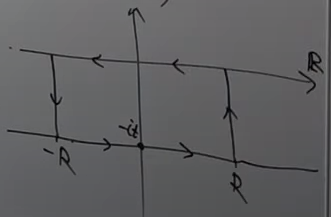
\includegraphics[width=8cm]{./assets/03-characteristic-funcs/complex-arbitrary-value-example-1.png}
    \end{center}

    $(*): \left| \int_{R - it}^{R} e^{-\frac{z^2}{2}} dz \right| =_{z = R + i y} \left| i \int_{-t}^{0} e^{- \frac{(R + iy)^2}{2}} dy \right| \leq \int_{-t}^{0} |\ldots|dy = \int_{-t}^{0} e^{\frac{-R^2 + y^2}{2}} dy \leq t e^{\frac{t^2}{2}} e^{\frac{-R^2}{2}} \rightarrow_{R \to \infty} 0$.


    Тогда получаем, что $I = \sqrt{2 \pi}$, и $\phi_{\eta}(t) = e^{-\frac{t^2}{2}}$.


    Теперь находим $\phi_{\xi}(t) = e^{iat} \phi_{\eta}(\sigma t) = e^{- \frac{\sigma^2 t^2}{2} + iat}$.
\end{example}

\begin{theorem}
    Пусть $\mathbb{E} |\xi|^n < +\infty$.

    Тогда при $k \leqslant n$ верно, что $\varphi^{(k)} (t) = \mathbb{E} ((i\xi)^k e^{i\xi t}) $.

    В частности, $\varphi^{(k)} (0) = i^k \mathbb{E} \xi^k$.

    \textit{Тут имеется в виду $k$-ая производная.}
\end{theorem}

\begin{consequence}
    Если $\mathbb{E} \xi^2 < + \infty$, то $\mathbb{E} \xi = -i \varphi'(0)$ и $\mathbb{D} \xi = -\varphi''(0) + (\varphi'(0))^2$
\end{consequence}

\begin{proof}
    Теоремы.

    Индукция по $k$

    База $k = 0$: определение $\varphi$.

    Переход $k \to k + 1$:

    $\varphi^{(k + 1)}(t) = \lim_{h \to 0} \frac{\varphi^{(k)}(t + h) - \varphi^{(k)}(t)}{h} = $

    $= \lim_{h \to 0} \frac{\mathbb{E} (i \xi)^k e^{i\xi(t + h)} - \mathbb{E} (i \xi)^k e^{it\xi}}{h} =
    \lim_{h \to 0} \mathbb{E} ((i \xi)^k e^{i t \xi} \cdot \frac{e^{ih\xi} - 1}{h}) = \mathbb{E} ((i\xi)^k e^{i t \xi} \cdot \lim_{h \to 0} \frac{e^{i h \xi} - 1}{h})$, а предел -- это $i \xi$.

    Почему можно было запихать предел под матожидание?

    $\lim \int_{\mathbb{R}} (ix)^k e^{itx} \frac{e^{ihx} - 1}{h} d P_{\xi}(x) = \int_{R} \lim_{h \to 0} ((ix)^k e^{itx} \frac{e^{ihx} - 1}{h}) d P_{\xi}(x)$ -- нужна суммируемая мажоранта.

    $\left | (ix)^k e^{itx} \frac{e^{ihx} - 1}{h}  \right | = |x|^k \left | \frac{e^{ihx} - 1}{h} \right | = (*)$.

    \begin{enumerate}
        \item {
            Если $|xh| \geqslant 1$, то $\left | \frac{e^{ihx} - 1}{h} \right | \leqslant \frac{2}{|h|} \leqslant 2|x| $ и тогда $(*) \leq 2|x|^{k + 1}$.
        }
        \item {
            Если $|xh| < 1$, то $e^{ihx} = 1 + \mathcal{O}(1 + ihx) \Rightarrow \left | \frac{e^{ihx} - 1}{h}  \right | = \left | \frac{\mathcal{O}(hx)}{h}  \right | = \mathcal{O}(x)$ и тогда $(*) = \mathcal{O}(|x|^{k + 1})$.
        }
    \end{enumerate}

    Но $\int_{\mathbb{R}} |x|^{k + 1} d P_{\xi} (x) = \mathbb{E} |\xi|^{k + 1} < +\infty$ по условию, тогда мажоранту подобрали правильную.
\end{proof}

\begin{theorem}
    Если существует $\varphi_{\xi}''(0)$ и конечна, то $\mathbb{E} \xi^2 < +\infty$
\end{theorem}

\begin{remark}
    Если существует $\varphi_{\xi}^{(2n)}$ и конечна, то $\mathbb{E} \xi^{2n} < +\infty$
\end{remark}

\begin{proof}
    $\mathbb{E} \xi^2 = \int_{\mathbb{R}} x^2 dP_{\xi} (x) = (*)$ -- хотим доказать, что этот интеграл конечен.

    Заметим, что $x = \lim_{t \to 0} \frac{\sin (tx)}{t}$ и подставим вместо $x$.

    Тогда:

    $(*) = \int_{\mathbb{R}} \lim_{t \to 0} \frac{\sin^2 (tx)}{t^2} dP_{\xi}(x) \leqslant
    \underline{\lim}_{t \to 0} \int_{\mathbb{R}} -\frac{e^{2itx} + e^{-2itx} - 2}{4t^2} dP_{\xi} (x) = (*)$ -- лемма Фату и расписали синус как $\sin{a} = \frac{e^{ia} - e^{-ia}}{2 i}$.

    $(*) = \underline{\lim}_{t \to 0} -\frac{\varphi_{\xi}(2t) - \varphi_{\xi}(-2t) - 2}{4t^2} = (*)$.

    Причём $\varphi_{\xi} (u) = \varphi_{\xi}(0) + \varphi_{\xi}'(0) \cdot u + \frac{\varphi_{\xi}''(0) u^2}{2} + o(u^2)$.

    Тогда $\varphi_{\xi}(2t) + \varphi_{\xi}(-2t) = 2 + \frac{\varphi_{\xi}''(0) \left((2t)^2 + (-2t)^2 \right)}{2} + o(t^2)$, а тогда $(*) = \underline{\lim}_{t \to 0} (-\varphi_{\xi}''(0) + o(1))$.

    То есть оценили сверху каким-то число, тогда интеграл конечен.
\end{proof}

\begin{theorem}
    \textbf{Формула обращения}

    Пусть $a < b$ и $P(\xi = a) = P(\xi = b) = 0$.

    Тогда $P(\xi \in [a, b]) = \lim_{T \to +\infty} \frac{1}{2\pi} \int_{-T}^{T} \frac{e^{-iat} - e^{-ibt}}{it} \varphi_{\xi}(t) \, dt $

    То есть $v.p. \frac{1}{2\pi} \int_{\mathbb{R}} \frac{e^{-iat} - e^{-ibt}}{it} \varphi_{\xi}(t) \, dt$
\end{theorem}

\begin{proof}

    Будем доказывать в несколько шагов:

    \begin{enumerate}
        \item {
            Пусть $\xi = \frac{b - a}{2} \eta + \frac{a +  b}{2}$, $\xi \in [a, b] \Leftrightarrow \eta \in [-1, 1]$, тогда $P(\xi \in [a, b]) = P(\eta \in [-1, 1]) = (')$.

            Допустим, что мы уже доказали эту формулу для $\eta \in [-1, 1]$, тогда

            $P(\eta \in [-1, 1]) = \lim_{T \to +\infty} \frac{1}{2\pi} \int_{-T}^{T} \frac{e^{-it} - e^{i t}}{it} \phi_{\eta}(t) dt = (*)$

            Пересчитаем левую часть формулы $(')$:

            $P(\xi \in [a, b]) = \lim_{T \to +\infty} \frac{1}{2\pi} \int_{-T}^{T} \frac{e^{i a t} - e^{i b t}}{i t} \phi_{\eta} (\frac{b - a}{2} t) e^{i \frac{a + b}{2} t} dt =_{s := \frac{b - a}{2} t}$

            $= \lim_{T \to +\infty} \frac{1}{2 \pi} \int_{-T \frac{b - a}{2}}^{T \frac{b - a}{2}} \frac{e^{i s} - e^{-i s}}{is} \phi_{\eta}(s) ds = (**)$

            То есть если мы получили, что $(*) = (**)$.

            Тогда если мы докажем формулу при $\eta \in [-1, 1]$, то решим задачу.
        }
        \item {
            Пусть $a = -1, b = 1$:

            $P(\xi \in [-1, 1]) \overset{?}{=} \lim_{T \to +\infty} \frac{1}{2\pi} \int_{-T}^{T} \frac{e^{it} - e^{-it}}{it} \phi_{\xi}(t) dt$.

            Посчитаем интеграл:

            $\int_{-T}^{T} \frac{e^{it} - e^{-it}}{it} \phi_{\xi}(t) dt = \int_{-T}^{T} \frac{e^{it} - e^{-it}}{it} \int_{\mathbb{R}} e^{itx} dP_{\xi}(x) dt =_{\text{т. Фубини}} \int_{\mathbb{R}} \int_{-T}^{T} \frac{e^{it} - e^{-it}}{it} e^{i t x} dt dP_{\xi}(x)$ -- теорему Фубини можно применять, если подъинтегральная функция суммируема: $|e^{i t x}| < 1$ и $|\frac{e^{it} - e^{-it}}{it}|$ -- ограничена (при больших $t$ значение меньше $2$, при $t \in [-1, 1]$ это непрерывная функция, а значит ограничена на этом отрезке).

            Давайте посмотрим на внутренний интеграл: $\Phi_{T}(x) = \int_{-T}^{T} \frac{e^{it} - e^{-it}}{it} e^{it x} dt$.

            Заметим, что $\frac{e^{it} - e^{-it}}{it} = \int_{-1}^{1} e^{i t u} du$.

            Тогда $\Phi_{T}(x) = \int_{-T}^{T} \int_{-1}^{1} e^{i t u} e^{i t x} du dt = \int_{-1}^{1} \int_{-T}^{T} e^{i t (u + x)} dt du$ -- т. Фубини, т.к. подъинтегральная ф-я по модулю равна $1$.


        }
    \end{enumerate}



    % $\xi = \frac{a + b}{2} + \frac{b - a}{2}\eta$, тогда $P(\xi \in [a, b]) = P(\eta \in [-1, 1])$, в частности $P_{\eta}(\{ \pm 1 \}) = 0$.

    % $\varphi_{\xi}(t) = e^{i \frac{a + b}{2} t} \varphi_{\eta}(\frac{b - a}{2}t)$ - подставим в наш интеграл.

    % $ \int_{-T}^{T} \frac{e^{-iat} - e^{-ibt}}{it} \varphi_{\xi} (t) \, dt = \int_{-T}^{T} \frac{e^{-iat} - e^{-ibt}}{it} e^{i \frac{a + b}{2} t} \varphi_{\eta} (\frac{b - a}{2} t) \, dt = $

    % $ = \int_{-T}^{T} \frac{e^{-i\frac{a - b}{2}t} - e^{-i\frac{b - a}{2}t}}{it} \varphi_{\eta} (\frac{b - a}{2}) \, dt = \int_{-\frac{b - a}{2}T}^{\frac{b - a}{2}T} \frac{e^{is} - e^{-is}}{is} \varphi_{\eta} (s) \, ds$, здесь замена $s = \frac{b - a}{2} t$

    % Можно считать, что $a = -1$, а $b = 1$

    % $\int_{-T}^T \frac{e^{it} - e^{-it}}{it} \varphi_{\xi}(t) \, dt = \int_{-T}^T \int_{\mathbb{R}} \frac{e^{it} - e^{-it}}{it} e^{itx} dP_{\xi}(x) \, dt = (*)$ - давайте переставим местами интегралы.

    % Нужна суммируемость того, что под интегралом, а она есть, всё ограничено какой-то суммируемой константой.

    % $(*) = \int_{\mathbb{R}} \int_{-T}^T \frac{e^{it} - e^{-it}}{it} e^{itx} \, dt \, dP_{\xi}(x)$.  Пусть $\Phi_T (x) = \int_{-T}^{T} \frac{e^{it} - e^{-it}}{it} e^{itx} \, dt$

    % $\lim_{T \to +\infty} \int_{-T}^T \frac{e^{it} - e^{-it}}{it} \varphi_{\xi} (t) \, dt = \lim_{T \to +\infty} \int_{\mathbb{R}} \Phi_T(x) dP_{\xi} (x) = \int_{\mathbb{R}} \lim_{T \to +\infty} \Phi_T (x) \, dP_{\xi} (x) $ - хотим понять, почему
    % можно внести предел под интеграл, но разберемся с этим позже.

    % $\lim_{T \to +\infty} \Phi_T (x) = \lim_{T \to +\infty} \int_{-1}^1 \int_{-T}^T e^{it(u + x)} \, dt \, du = (*)$.

    % Заметим, что $\frac{e^{it(u + x)}}{i(u + x)} \bigg |_{t = -T}^{t = +T} = \frac{2\sin ((u + x)T)}{u + x}$ -- первообразная для внутреннего интергала $(*)$.

    % Тогда $(*) = \lim_{T \to +\infty} \int_{-1}^1 \frac{2\sin ((u + x)T)}{u + x} \, du = (*)$. Сделаем замену $y = (u + x)T$, тогда $dy = T \cdot du$.

    % Тогда $(*) = \lim_{T \to +\infty} \int_{(-1 + x)T}^{(1 + x)T} \frac{2 \sin y}{y} \, dy = \begin{cases}
    %     0, & \text{при $x > 1$} \\
    %     0, & \text{при x < -1} \\
    %     \int_{\mathbb{R}} \frac{2 \sin y}{y} \, dy = 2\pi, & \text{иначе}
    % \end{cases}$

    % Получили $2\pi \int_{\mathbb{R}} \mathds{1}_{[-1, 1]} (x) \, dP_{\xi} (x) = 2\pi P_{\xi}([-1, 1])$.

    % Вспомним, что мы не доказали по дороге один переход. Нужно понять, почему $\int_{a}^b \frac{\sin y}{y} \, dy$ ограничен - интеграл по лучу сходится, значит первообразная
    % в бесконечностях имеет предел, значит в середине тоже ограничена, потому что непрервность - обоснование примерно такое.


    $\lim_{T \to +\infty} \Phi_T (x) = \lim_{T \to +\infty} \int_{-1}^1 \int_{-T}^T e^{it(u + x)} \, dt \, du = (*)$.

    Заметим, что $\frac{e^{it(u + x)}}{i(u + x)} \bigg |_{t = -T}^{t = +T} = \frac{2\sin ((u + x)T)}{u + x}$ -- первообразная для внутреннего интергала $(*)$.

    Тогда $(*) = \lim_{T \to +\infty} \int_{-1}^1 \frac{2\sin ((u + x)T)}{u + x} \, du = (*)$. Сделаем замену $y = (u + x)T$, тогда $dy = T \cdot du$.

    Тогда $(*) = \lim_{T \to +\infty} \int_{(-1 + x)T}^{(1 + x)T} \frac{2 \sin y}{y} \, dy = \begin{cases}
        0, & \text{при $x > 1$} \\
        0, & \text{при x < -1} \\
        \int_{\mathbb{R}} \frac{2 \sin y}{y} \, dy = 2\pi, & \text{иначе}
    \end{cases}$

    Получили, что $\lim_{T \to \infty} \Phi_T(x) = 2 \pi \cdot \mathds{1}_{[-1, 1]} (x)$.

    Если докажем, что $\int_{\mathbb{R}} \Phi_{T} (x) d P_{\xi}(x) \underbrace{\to_{\text{почти везде}}}_{\text{пользуемся } P(\xi = a) = P(\xi = b) = 0 } \int_{\mathbb{R}} 2 \pi \cdot \mathds{1}_{[-1, 1]} (x) d P_{\xi}(x)$, то решим задачу, т.к. правая часть это как раз $2 \pi P(\xi \in [-1, 1])$.

    То есть нужно понять, почему $\int_{a}^b \frac{\sin y}{y} \, dy$ ограничен -- интеграл по лучу сходится, значит первообразная в бесконечностях имеет предел, значит в середине тоже ограничена, потому что непрервность -- обоснование примерно такое.

\end{proof}

\begin{consequence}
    \begin{enumerate}
        \item {
            Если $\varphi_{\xi}(t) = \varphi_{\eta}(t)$, то $P_{\xi} = P_\eta$

            \textit{Доказательство: } Рассмотрим $A = \{ a \in \mathbb{R} \, : \, \text{$a$ - точка непрервности функции распределения} \}$.

            Тогда $\mathbb{R} \setminus A$ - не более чем счётное.
            Если $a < b$ и $a, b \in A$, то $P_{\xi} ([a, b]) = P_\eta ([a, b])$

            \begin{enumerate}
                \item {
                    Пусть $a \in \mathbb{R}, b \in A$:

                    Рассмотрим $a_n \in A$, такие, что $a_n \to a$ и убывают.

                    $P_{\xi} ((a, b]) = \lim_{n \to \infty} P_{\xi} ([a_n, b_n]) = \lim P_{\eta} ([a_n, b_n]) = P_\eta ((a, b])$.
                }
                \item {
                    Пусть $a < b$ произвольные:

                    Возьмём $b_n \in A$, такие, что $b_n \to b$ и убывают. Тогда $P_{\xi} ((a, b]) = \lim_{n \to \infty} P_{\xi} (a, b_n] = \lim P_\eta (a, b_n] = P_\eta (a, b] \Rightarrow
                    P_\xi = P_\eta$ на ячейках, а тогда по единственности продолжения везде совпадают.
                }
            \end{enumerate}
        }

        \item {
            Если $\int_{\mathbb{R}} |\varphi_\xi (t) | \, dt < +\infty$, то $\xi$ имеет плотность распределения
            $p_{\xi} (x) = \frac{1}{2\pi} \int_{\mathbb{R}} e^{-itx} \varphi_{\xi} (t) \, dt$ - преобразование Фурье.

            \textit{Доказательство: } Из суммируемости $\varphi_\xi (t) \Rightarrow P_{\xi} ((a, b]) = \frac{1}{2\pi} \int_{-\infty}^{+\infty} \frac{e^{-iat} - e^{-ibt}}{it} \varphi_{\xi} (t) \, dt$.

            Проверим, что $P_{\xi} (a, b] = \int_a^b p_{\xi} (x) \, dx$.

            $\int_a^b p_{\xi} (x) \, dx = \frac{1}{2\pi} \int_a^b \int_{\mathbb{R}} e^{-itx} \varphi_\xi (t) \, dt \, dx = (*)$. Под внутренним интегралом суммируемая функция, значит можно переставлять местми интегралы.

            Тогда $(*) = \frac{1}{2\pi} \int_{\mathbb{R}} \int_a^b e^{-itx} \, dx \varphi_\xi (t) \, dt$
        }
    \end{enumerate}
\end{consequence}

\begin{theorem}
    $\xi_k \sim \mathcal{N} (a_k, \sigma_k^2)$, $c_k \in \mathbb{R}$ не все нулевые и $\xi_k$ -- независимы и $\xi = a_0 + \sum_{k = 1}^n c_k \xi_k$.

    Тогда $\xi \sim \mathcal{N} (a, \sigma^2)$, где
    $a = a_0 + \sum_{k = 1}^n c_k a_k$ и $\sigma^2 = \sum_{k = 1}^n c_k^2 \sigma_k^2$.
\end{theorem}

\begin{proof}
    $\varphi_{\xi} (t) = \varphi_{a_0} (t) \varphi_{c_1\xi_1} (t) \ldots \varphi_{c_n\xi_n} (t) = $

    $=  e^{ita_0} (t) \varphi_{\xi_1} (c_1t) \ldots \varphi_{\xi_n} (c_nt) =
    e^{ita_0} e^{ia_1c_1 t} e^{- \frac{(c_1 \sigma_1 t)^2}{2}} \ldots e^{ia_nc_n t} e^{- \frac{(c_n \sigma_n t)^2}{2}} =
    e^{ita} e^{- \frac{\sigma^2t^2}{2}} $
\end{proof}

\Subsection{Сходимость по распределению}

\begin{remark}
    \begin{enumerate}
        \item {
            Точек, где нет непрерывности $F_{\xi}$ не более чем счётное множество

            %\begin{proof}
            %    $P(\xi = x) > 0$ - эти точки, а мера вероятностная.
            %\end{proof}
        }
        \item {
            Если $F_{\xi_n}(b) - F_{\xi_n} (a) \rightarrow F_{\xi}(b) - F_{\xi}(a)$ для всех $a, b$, за исключением счётного множества.

            Тогда $F_{\xi_n}(b) \rightarrow F_{\xi} (b)$ за исключением счётного множества.

            \begin{proof}
                Рассмотрим $F(x)$, функцию распределения. Возьмём хорошие $a$, т.ч. $F(a) < \varepsilon$ и
                $b$, т.ч. $F(b) > 1 - \varepsilon$.

                Тогда $(F_n(b) - F_n (a)) - (F(b) - F(a)) \rightarrow 0 \implies
                |(F_n(b) - F_n(a)) - \underbrace{(F(b) - F(a))}_{> 1 - 2\varepsilon}| < \varepsilon \implies F_n(b) - F_n(a) > 1 - 3\varepsilon \implies F_n(a) < 3\varepsilon$ при больших $n$.

                Возьмём хорошее $x$, $|F_n(x) - F(x)| \leqslant |(F_n(x) - F_n(a)) - (F(x) - F(a))| + \underbrace{F_n(a)}_{<3\varepsilon} + \underbrace{F(a)}_{<\varepsilon} < 5\varepsilon$ при больших $n$
            \end{proof}
        }
        \item {
            $D \subset \mathbb{R}$ не более чем счётное и $U \subset \mathbb{R}$ - открытое.

            Тогда $U = \bigcup_{k = 1}^{\infty} (a_k, B_k]$, где $a_k, b_k \not \in D$

            \begin{proof}
                Нарезаем открытое множество с шагом 1, тем ячейки, которые целиком попали - берём. Те, что не попали - бьём пополам и так далее.
            \end{proof}
        }
        \item {
            $\xi$ и $\eta$ независимые и $\eta$ имеет непрерывное распределение.

            Тогда $\xi + \eta$ имеет непрерывное распределение.

            \begin{proof}
                $P_{\xi + \eta} = P_{\xi} * P_{\eta}$

                $P_{\xi + \eta} (\{ a \}) = \int_{\mathbb{R}} \underbrace{P_{\eta} ( \{ a - x \} )}_{= 0, \text{т.к. непрерывность}}  dP_{\xi} (x) $
            \end{proof}
        }
    \end{enumerate}
\end{remark}

\begin{definition}
    Множество $B \subset \mathbb{R}$ - регулярное, относительно $P_{\xi}$, если $P_{\xi} (Cl \, B \setminus Int \, B) = 0$,
    то есть $P(\xi \in Cl \, B \setminus Int \, B) = 0$
\end{definition}

\begin{theorem}
    $\xi, \xi_1, \xi_2, \ldots$ - случаный величины, $F, F_1, F_2, \ldots$ - их функции распределения, а
    $\varphi, \varphi_1, \varphi_2, \ldots$ - их характеристичечкие функции. Следующие условия равносильны:

    \begin{enumerate}
        \item $\xi_n$ сходится к $\xi$ по распределению
        \item Для любого $U$ открытого $\underline{\lim} P(\xi_n \in U) \geqslant P(\xi \in U)$
        \item Для любого $A$ замкнутого $\overline{\lim} P(\xi_n \in A) \leqslant P(\xi \in A)$
        \item Для любого $B$ регулярного борелевского $\lim P(\xi_n \in B) = P(\xi \in B)$
        \item Для любого $B$ регулярного борелевского $\lim \mathbb{E} \mathds{1}_{B}(\xi_n) = \mathbb{E} \mathds{1}_B (\xi)$
        \item Для любой $f$ непрерывной на прямой и ограниченной $\lim \mathbb{E} f(\xi_n) = \mathbb{E} f(\xi)$
        \item $\varphi_n$ сходится к $\varphi$ поточечно
    \end{enumerate}
\end{theorem}

\begin{proof}
    \begin{enumerate}
        \item {
            $2 \Longleftrightarrow 3$

            Если $A = \mathbb{R} \setminus U$, тогда $P(\xi_n \in A) = 1 - P(\xi_n \in U)$.

            $P(\xi \in A) > \overline{\lim} P(\xi_n \in A) = 1 - \underline{\lim} P(\xi_n \in U) \leqslant 1 - P(\xi \in U) = P(\xi \in A)$
        }
        \item {
            $2 \cup 3 \implies 4$

            Мы знаем, что $U = \{ \xi_n \in Int \, B \} \{ \xi_n \in B \} \subset \{ \xi_n \in Cl \, B \} = A$

            Тогда $P(\xi_n \in U) \leqslant P(\xi_n \in B) \leqslant P(\xi_n \in A) \implies \underbrace{\overline{\lim} P(\xi_n \in B)}_{\geqslant \underline{\lim} P(\xi_n \in B) \geqslant \underline{\lim} P(\xi_n \in U) \geqslant P(\xi \in U) = P(\xi \in B)} \leqslant \overline{\lim} P(\xi_n \in A) \leqslant P(\xi \in A) = P(\xi \in B)$
        }
        \item {
            $4 \Longleftrightarrow 5$

            $\mathbb{E} \mathds{1}_B (\xi_n) = P(\mathds{1}_B (\xi_n) = 1) = P(\xi_n \in B)$
        }
        \item {
            $6 \implies 7$

            $\varphi_{\eta} (t) = \mathbb{E} e^{et\eta} = \mathbb{E} \cos (t\eta) + i \mathbb{E} \sin (t \eta)$

            Тогда $\varphi_n(t) = \mathbb{E} \cos (t \xi_n) + i\mathbb{E} \sin (t\xi_n) \rightarrow \mathbb{E} \cos (t\xi) + i \mathbb{E} \sin (t\xi) = \varphi (t)$
        }
        \item {
            $1 \implies 2$

            Берём открытое $U$, по замечанию $U =  \bigcup\limits_{k = 1}^{\infty} (a_k, b_k]$, где $a_k, b_k$ - точки непрерывности $F$.

            $\{ \xi_n \in U \} \supset \{ \xi_n \in \bigcup\limits_{k = 1}^{m} (a_k, b_k] \} \implies P(\xi_n \in U) \geqslant \sum_{k = 1}^m P(\xi_n \in (a_k, b_k])$

            $\underline{\lim} P(\xi_n \in U) \geqslant \underline{\lim} \sum_{k  = 1}^m \geqslant \sum_{k = 1}^m \underline{\lim} P(\xi_n \in (a_k, b_k]) \overset{*}{=} \sum_{k = 1}^m P(\xi \in (a_k b_k]) \overset{m \to \infty}{\rightarrow} \sum_{k = 1}^{\infty} P(\xi \in (a_k, b_k]) = P(\xi \in U)$

            А значит $\underline{\lim} P(\xi_n \in U) \geqslant P(\xi \in U)$

            $(*) P(\xi_n \in (a_k, b_k]) = F_n (b_k) - F_n (a_k) \rightarrow F(b_k) - F(a_k) = P(\xi \in (a_k, b_k])$
        }
        \item {
            $5 \implies 6$

            Пусть $|f| \leqslant M$ и $D = \{ x \in \mathbb{R} \, : \, P(f(\xi) = x) > 0 \} = \{ x \, : \, P_{\xi} (f^{-1} (x) > 0) \}$. Это не более чем счётное множество. Потому что для разных $x$ - это дизъюнктные.
            Множеств с вероятностью $\frac{1}{2}$ - не больше двух, с вероятностью $\frac{1}{3}$ не больше трёх и так далее.

            Пусть $-M = t_0 < t_1 < \ldots < t_m = M$, так, что $t_y \not \in D$ и мелкость $< \varepsilon$.

            Заведём множества $A_j = \{ x \in \mathbb{R} \, : \, t_{j - 1} \leqslant f(x) \leqslant t_j \} \supset B_j = \{ x \in \mathbb{R} \, : \, t_{j - 1} < f(x) \leqslant t_j \} \supset U_j = \{ x \in \mathbb{R} \, : \, t_{j - 1} < f(x) < t_j \}$. Где $A_j$ - замкнутое,а $U_j$ - открытое.

            Мы поняли, что $U_j \subset Int \, B_j \subset B_j \subset Cl \, B_j \subset A_j \implies Cl \, B_j \setminus Int \, B_j \subset A_j \setminus U_j$

            Тогда $B_j$ регулярно относительно $P_\xi$

            Определим $g(x) = \sum_{j = 1}^{m} t_{j - 1} \mathds{1}_{B_j} (x)$. Тогда $g(x) < f(x) < g(x) + \varepsilon$.

            $|g(x) - f(x)| < \varepsilon$ и тогда $\mathbb{E} |g(\xi_n) - f(\xi_n)| \leqslant \varepsilon$ и мы знаем, что $\mathbb{E}g(\xi_n) \rightarrow \mathbb{E}g(\xi)$ - видно, если расписать матожидание $g$ по линейности.

            $\mathbb{E} |f(\xi_n) - f(\xi)| \leqslant |\mathbb{E} f(\xi_n) - \mathbb{E} g(\xi_n)| + |\mathbb{E} g(\xi_n) - \mathbb{E} g(\xi)| + |\mathbb{E} g(\xi) - \mathbb{E} f(\xi) | < 3\varepsilon$ при больших $n$, каждый из модулей $< \varepsilon$
        }
        \item {
            $7 \implies 1$

            Возьмём $\eta \sim \mathcal{N} (0, \sigma^2)$, такую, что $\eta$ не зависит от всех $\xi_n$ и $\xi$

            $\varphi_{\xi_n + \eta} (t) = \varphi_{\xi_n} (t) \varphi_{\eta} (t) = \varphi_{n} (t) \cdot e^{-\frac{\sigma^2 t^2}{2}} \overset{\text{поточечно}}{\rightarrow} \varphi(t) e^{-\frac{\sigma^2t^2}{2}} = \varphi_{\xi + \eta} (t)$

            $\xi_n + \eta$ и $\xi + \eta$ имеют непрерывное распределение, поэтому можем не задумываясь писать формулу обращения:

            $P(\xi_n + \eta \in (a, b]) = \frac{1}{2\pi} \int_{\mathbb{R}} \frac{e^{-iat} - e^{-ibt}}{it} \varphi_{\xi_n + \eta} (t) \, dt \overset{*}{\rightarrow} \frac{1}{2\pi} \int_{\mathbb{R}} \frac{e^{-iat} - e^{-ibt}}{it} \varphi_{\xi + \eta} \, dt = P(\xi + \eta \in (a, b])$.

            $(*)$ Нужна суммируемая мажоранта $\left | \frac{e^{-iat} - e^{-ibt}}{it} \varphi_{\xi_n + \eta} (t) \right | \leqslant e^{-\frac{\sigma^2t^2}{2}}$ - суммируемая мажоранта.

            То есть $\underbrace{P(\xi_n + \eta \in (a, b])}_{G_n (b) - G_n(a)} \rightarrow \underbrace{P(\xi + \eta \in (a, b])}_{G(b) - G(a)}$, где $G_n (x) = F_{\xi_n + \eta}(x)$ и $G(x) = F_{\xi + \eta} (x)$

            Тогда из замечания $G_n(x) \rightarrow G(x)$

            Возьмём $x$ - точка непрерывности $F$ и выберем $\delta > 0$, так, что $|F(x \pm \delta) - F(x)| < \varepsilon$ - есть из непрерывности.

            $ \{ \xi_n + \eta \leqslant x - \delta \} \setminus \{ |\eta| > \delta \} \subset  \{ \xi_n \leqslant x \} \subset \{ \xi_n + \eta \leqslant x + \delta \} \cup \{ |\eta| > \delta \}$.

            Тогда $\underbrace{G_{n} (x - \delta) - P(|\eta| > \delta)}_{G_n (x - \delta - \frac{\sigma^2}{\delta^2}) > G_n (x - \delta) - \varepsilon > G(x - \delta) - 2\varepsilon > F(x - 2\delta) - 3\varepsilon > F(x) - 4\varepsilon} \leqslant F_n (x) \leqslant
            \underbrace{G_{n} (x + \delta) + P(|\eta| > \delta)}_{G_n (x + \delta) + \frac{\sigma^2}{\delta^2} < G_n (x + \delta) + \varepsilon < G(x + \delta) + 2\varepsilon < F(x + 2\delta) + 3\varepsilon < F(x) + 4\varepsilon}$

            Оценим вероятность: $P(|\eta| > \delta) \leqslant \frac{\mathbb{D} \eta}{\delta^2} = \frac{\sigma^2}{\delta^2}$


        }
    \end{enumerate}
\end{proof}

\begin{theorem}
    $F_n, F \, \mathbb{R} \to [0, 1]$ монотонные, $F \in C(\mathbb{R})$ и
    $F_n \to F$ поточечно.

    Тогда $F_n \rightrightarrows F$
\end{theorem}

\begin{proof}
    Берём $\varepsilon > 0$ и $m > \frac{1}{\varepsilon}$. Пусть $t_j$, такие, что $F(t_j) = \frac{j}{m}$. Если для большого $j$ точки не нашлось, то
    $F < \frac{j + 1}{m}$, а если для маленького не нашлось, то $F > \frac{j - 1}{m}$ (потому что иначе из непрерывности такие точки найдутся).

    Знаем, что $F_n(t_j) \rightarrow F(t_j)$. Берём $N \, : \, \forall \, n \geqslant N \, |F_n(t_j) - F(t_j)| < \varepsilon$.

    Теперь смотрим на произвольную точку: $t_j < t < t_{j + 1}$. Тогда
    $F_n(t) \leqslant F_n(t_{j + 1}) < F(t_{j + 1}) + \varepsilon = \frac{j + 1}{m} + \varepsilon = F(t_j) + \frac{1}{m} + \varepsilon \leqslant F(t) + \frac{1}{m} + \varepsilon < F(t) + 2\varepsilon$.

    Аналогично в другую сторону:

    $F_n (t_j) > F(t_j) - \varepsilon = \frac{j}{m} - \varepsilon = F(t_{j + 1}) - \frac{1}{m} - \varepsilon \geqslant F(t) - 2\varepsilon$.

\end{proof}

\Subsection{Центральная предельная теорема}

\begin{theorem}
    \textbf{ЦПТ в форме Леви}

    $\xi_1, \xi_2, \ldots $ независимые, одинаково распределённые случайные величины. $a = \mathbb{E} \xi_1,
    \sigma^2 = \mathbb{D} \xi_1, S_n = \xi_1 + \xi_2 + \ldots + \xi_n$.

    Тогда $P \left ( \frac{S_n - nq}{\sigma \sqrt{n}} \leqslant x \right ) = P\left ( \frac{S_n - \mathbb{E} S_n}{\sqrt{\mathbb{D} S_n}} \leqslant x \right ) \rightrightarrows \Phi (x) = \frac{1}{\sqrt{2\pi}} \int_{-\infty}^x e^{-\frac{t^2}{2}} \, dt$
\end{theorem}

\begin{proof}
    Достаточно проверять поточечную сходимость характеристических функций.

    $\varphi_{\xi_k - a} (t) = 1 - \frac{\sigma^2 t^2}{2} + o(t^2)$, потому что
    мы знаем, что $\mathbb{E} (\xi_k - a) = 0$ и $\mathbb{D} (\xi_k - a) \sigma^2$

    Тогда $\varphi_{S_n - na} (t) = \prod\limits_{k = 1}^n \varphi_{\xi_k - a} (t) = \left ( 1 - \frac{\sigma^2t^2}{2} + o(t^2) \right )^n$

    $\varphi_{\frac{S_n - na}{\sigma \sqrt{n}}} = \varphi_{S_n - na} \left ( \frac{t}{\sqrt{n}\sigma} \right ) = \left( 1 - \frac{t^2}{2n} + o(\frac{t^2}{n}) \right) \rightarrow e^{-\frac{t^2}{2}}$.

    Чтобы получить последний переход - логарифмируем.

    То есть $\frac{S_n - na}{\sqrt{n} \sigma}$ сходится по распределению к $\mathcal{N} (0, 1) \implies$ функция распределения сходится равномерно.
\end{proof}

\begin{consequence}
    \textbf{Интегральная теорема Муавра-Лапласа}

    $S_n$ - количество успехов в схеме Бернулли с вероятностью успеха $p \in (0, 1)$.

    Тогда $P \left( \frac{S_n - np}{\sqrt{npq}} \leqslant \right) \rightrightarrows \Phi (x)$
\end{consequence}

\begin{proof}
    $\mathbb{E} \xi_k = p, \mathbb{D} \xi_k = pq$
\end{proof}

\begin{example}
    \textbf{Посчитаем характеристическую функцию для Poisson($\lambda$)}

    $\varphi_{\xi} (t) = \mathbb{E} e^{i t \xi} = \sum_{n = 0}^\infty e^{itn} \frac{e^-\lambda \lambda^n}{n!} = \sum_{n = 0}^\infty \frac{(\lambda e^{it})^n}{n!} \cdot e^{-\lambda} = exp (\lambda (e^{it} - 1))$
\end{example}

\begin{theorem}
    $P(\xi_{nk} = 1) = p_{nk}$ и $P(\xi_{nk} = 0) = 1 - p_{nk}$ и пусть $S_n = \xi_{n1} + \ldots + \xi_{nn}$.

    $\max \{ p_{n1}, \ldots, p_{nn} \} \rightarrow 0$ и $p_{n1} + \ldots p_{nn} \rightarrow \lambda$.

    Тогда $P(S_n = k) \rightarrow \frac{\lambda^k e^{-\lambda}}{k!}$
\end{theorem}

\begin{proof}
    $\varphi_{\xi_{nk}} (t) = \mathbb{E} e^{it\xi_{nk}} = 1 - p_{nk} + p_{nk}e^{it} = 1 + p_{nk} (e^{it} - 1)$

    Тогда $\varphi_{S_n} = \prod_{k = 1}^n (1 + p_{nk} (e^{it} - 1)) \overset{?}{\rightarrow} exp (\lambda (e^{it} - 1)) $.

    Пусть $z = e^{it} - 1$

    Значит, нужно проверить $\sum_{k = 1}^n \ln (1 + p_{nk} z) \rightarrow \lambda z$. Раскладываем логарифм:

    $\underbrace{\sum_{k = 1}^n p_{nk} z}_{\rightarrow \lambda z} + \sum_{k = 1}^n \mathcal{O} (p_{nk}^2)$. Значит осталось показать, что вторая сумма стремится к нулю.

    Действительно, $\sum_{k = 1}^n \mathcal{O} (p_{nk}^2) \leqslant (p_{n1} + \ldots p_{nn}) \cdot \max \{ p_{n1}, \ldots, p_{nn} \}  \rightarrow 0$
\end{proof}

\begin{theorem}
    \textbf{ЦПТ в форме Линденберга}

    $\xi_1, \ldots$ - независимые случайные величины, $a_k = \mathbb{E} \xi_k, \sigma_k^2 = \mathbb{D} \xi_k > 0, S_n = \xi_1 + \ldots + \xi_n, \mathbb{D}_n^2 = \sum_{k = 1}^n \sigma_k^2$

    $f(x) = x^2 \mathds{1}_{\{ |x| \geqslant \varepsilon \mathbb{D}_n \} } (x) \, \forall \, \varepsilon > 0$ и $Lind (\varepsilon, n) = \frac{1}{\mathbb{D}_n^2} \sum_{k = 1}^n \mathbb{E} f (\xi_k - a_k) \rightarrow 0$

    Тогда $P \left( \frac{S_n - \mathbb{E} S_n}{\sqrt{\mathbb{D} S_n}} \leqslant x \right) \rightrightarrows \Phi (x)$
\end{theorem}

\begin{theorem}
    \textbf{ЦПТ в форме Ляпунова}

    $\xi_1, \ldots$ независимые случайные величины

    $L(\delta, n) = \frac{1}{\mathbb{D}_n^{2 + \delta}} \sum_{k = 1}^n \mathbb{E} | \xi_k - a_k |^{2 + \delta} \rightarrow 0$ при некотором $\delta$

    Тогда $P\left( \frac{S_n - \mathbb{E} S_n}{\sqrt{\mathbb{D} S_n}} \leqslant x \right) \rightrightarrows \Phi (x)$
\end{theorem}

\begin{proof}
    %Ляпунов из Линденберга:
    % TODO
    %$Lind (\varepsilon, n) = \frac{1}{\mathbb{D}_n^2} \sum_{k = 1}^n \mathbb{E} (|\xi_k - a_k|^2 \cdot \mathds{1}_{|x| \geqslant \varepsilon \mathbb{D}_n} (\xi_k - a_k) ) \leqslant \frac{1}{\mathbb{D}_n^2} \sum_{k = 1}^n \mathbb{E} \left( \frac{|\xi_k - a_k|^{2 + \delta}}{} \right)$
\end{proof}

\begin{theorem}
    Пусть $\delta \in [0, 1]$ и $\xi_1, \ldots$ независимые случаные величины.

    Тогда $\left | P \left( \frac{S_n - \mathbb{E} S_n}{\sqrt{\mathbb{D} S_n}} \leqslant x \right) - \Phi (x) \right | \leqslant C_{\delta} L (\delta, n)$
\end{theorem}

\begin{theorem}
    \textbf{Берри-Эссенна}

    $\xi_1, \ldots$ независимые, одинаково распределённые случаные величины.

    Тогда$\left | P \left( \frac{S_n - na}{\sqrt{\sqrt{n} \sigma}} \leqslant x \right) - \Phi (x) \right | \leqslant C_{\delta} \cdot \frac{\mathbb{E} |\xi_1 - a|^{2 + \delta}}{n^{\frac{\delta}{2}} \sigma^{2 + \delta}}$
\end{theorem}

\begin{proof}
    $\mathbb{D}_n^2 = n \sigma^2$ и $L (\delta, n) = \frac{1}{n^{1 + \frac{\delta}{2} \cdot \sigma^{2 + \delta}}} \cdot n \mathbb{E} |\xi_1 - a|^{2 + \delta}$

    В частности при $\delta = 1 \, |P - \Phi| \leqslant C \frac{\mathbb{E} |\xi_1 - a|^3}{\sqrt{n} \sigma^3}$
\end{proof}

\begin{remark}
    \textbf{Про константы}

    \begin{enumerate}
        \item {
            Эссен (1956) $C \geqslant \frac{3 + \sqrt{10}}{6 \sqrt{2 \pi}} \approx 0,4097$
        }
        \item {
            Шевцова (2014) $C \leqslant 0,469$
        }
        \item {
            Для общего случая: $C_1 \leqslant 0,5583$
        }
        \item {
            Для схемы Бернулли (2018) $C_1 \leqslant 0,4099$
        }
        \item {
            Для схемы Бернулли с $p = \frac{1}{2}$ $C = \frac{1}{\sqrt{2\pi}}$
        }
    \end{enumerate}
\end{remark}

\begin{theorem}
    \textbf{Хартмана-Винтнера (закон повторного логарифма)}

    $\xi_1, \xi_2, \ldots$ - независимые, одинаково распределённые. $\mathbb{E} \xi_1 = 0, \, \mathbb{D} \xi_1 = \sigma^2 > 0$

    Тогда $\overline{\lim} \frac{S_n}{\sqrt{2n \ln \ln n}} = \sigma$, а $\underline{\lim} \frac{S_n}{\sqrt{2n \ln \ln n}} = -\sigma$
\end{theorem}

\begin{theorem}
    \textbf{Штрассена}

    $\xi_1, \xi_2 \ldots$ независимые одинаково распределённые, $\mathbb{E} \xi_1 = 0$ и $\mathbb{D} \xi_1 = \sigma^2 > 0$

    Тогда любое число из $[-\sigma, \sigma]$ - пред. точка послед. $\frac{S_n}{\sqrt{2n \ln \ln n}}$
\end{theorem}


\Subsection{Большие уклонения}

 \textbf{ЗБЧ в форме Чебышёва}

 $\xi_1, \xi_2, \ldots$ - незаисимые, одинаково распределённые случайные величины. $\mathbb{E} \xi_1 = a, \mathbb{D} = \sigma^2 > 0$

 Тогда $P\left(\frac{S_n}{n} \geqslant r \right) \rightarrow 0$, если $r > a$

 Более того, $P \left( \frac{S_n}{n} \geqslant r \right) \leqslant \frac{\sigma^2}{(r - a)n}$ - это оценка из доказательства. Но оценка довольно плохая.

 \begin{definition}
    $\xi$ удовлетворяет условию Крамера, если при $\lambda \in (0, \lambda_0)\, : \, \mathbb{E} e^{\lambda \xi} < +\infty$
 \end{definition}

 \begin{theorem}

    \textbf{Оценка Чернова}

    $\xi_1, \xi_2, \ldots$ - независимые, одинаково распределённые, удовлетворяющие условию Крамера и $r > a = \mathbb{E}\xi_1$

    Хотим оценить $P\left( \frac{S_n}{n} \geqslant r \right) = P\left( S_n \geqslant nr \right) = P\left( \lambda S_n \geqslant \lambda nr \right) = P\left( e^{ \lambda S_n} \geqslant e^{\lambda nr} \right) \overset{\text{Марков}}{\leqslant} \frac{\mathbb{E} e^{\lambda S_n}}{e^{\lambda n r}}
    \overset{*}{=} \left( \frac{\mathbb{E} e^{\lambda \xi_1}}{e^{\lambda r}}  \right)^n$

    $(*) \mathbb{E} e^{\lambda S_n} = \mathbb{E} (\prod_{k = 1}^n e^{\lambda \xi_k}) = (\mathbb{E} e^{\lambda \xi_1})^n$

    А теперь, то что получилось - будем минимизировать по $\lambda$

    $\varphi (\lambda) = \ln \mathbb{E} e^{\lambda \xi_1} - \lambda r \rightarrow \inf$, где $\lambda$ допустимое

    $I(r) = \sup_{\lambda} \{ \lambda r - \ln (\mathbb{E} e^{\lambda \xi_1}) \} \implies P \left( \frac{S_n}{n} \geqslant r \right) \leqslant e^{-n I(r)}$
 \end{theorem}

 \begin{example}
    \begin{enumerate}
        \item {
            $\xi \sim \mathcal{N} (0, 1)$

            $\mathbb{E} e^{\lambda \xi} = \frac{1}{\sqrt{2\pi}} \int_{\mathbb{R}} e^{\lambda x} e^{\frac{x^2}{2}} \, dx =
            \frac{1}{\sqrt{2\pi}} \int_{\mathbb{R}} e^{-\frac{(x - \lambda)^2}{2}} \, dx \cdot e^{\frac{\lambda^2}{2}} = e^{\frac{\lambda^2}{2}}$

            $\lambda r - \frac{\lambda^2}{2} \rightarrow \max\limits_{\lambda > 0}$, максимум при $\lambda = r$. И тогда $I(r) = \frac{r^2}{2}$

            Значит $P \left( \frac{S_n}{n} \geqslant r \right) \leqslant e^{-\frac{nr^2}{2}}$ при $r > 0$
        }
        \item {
            $\xi \sim Exp(1)$

            $\mathbb{E} e^{\lambda \xi} = \int_0^{+\infty} e^{\lambda x} e^{-x} \, dx = \frac{e^{(\lambda - 1)x}}{\lambda - 1} \bigg |_0^{+\infty} = \frac{1}{1 - \lambda}$ сходимость есть при $\lambda \in (0, 1)$

            $\lambda r - \ln \frac{1}{1 - \lambda} = \lambda r + \ln (1 - \lambda)$ - считаем производную по $\lambda$

            $(\lambda r + \ln (1 - \lambda))_\lambda' = r - \frac{1}{1 - \lambda} \implies 1 - \lambda = \frac{1}{r} \implies \lambda = 1 - \frac{1}{r}, r > 1$

            Тогда $I(r) = r (1 - \frac{1}{r}) - \ln r = r - 1 - \ln r$

            $P \left( \frac{S_n}{n} \geqslant r \right) \leqslant e^{-n (r -1 - \ln r)} = r^n e^{-n (r - 1)}$
        }
    \end{enumerate}
 \end{example}
\Section{Дискретные случайные процессы}{Виноградов Александр}
\Subsection{Условные математические ожидания}

\begin{definition}
    $(\Omega, \mathcal{F}, P)$ - вероятностное пространство, $\xi : \Omega \to \mathbb{R}$ и $\mathbb{E} |\xi| < +\infty$. Пусть $\mathcal{A} \subset \mathcal{F}$ и $\mathcal{A}$ - $\sigma-$алгебра.

    $\mathbb{E} (\xi | \mathcal{A}) = \eta \, : \, \Omega \to \mathbb{R}$ - случайная величина, которая:

    \begin{enumerate}
        \item измерима относительно $\mathcal{A}$
        \item $\forall \, A \in \mathbb{A} \, : \, \mathbb{E} (\xi \mathds{1}_A) = \mathbb{E} (\eta \mathds{1}_A)$
    \end{enumerate}
\end{definition}

\begin{theorem}
    $\mathcal{A} \subset \mathcal{F}, \mathbb{E} |\xi| < +\infty$, тогда $\mathbb{E} (\xi | \mathcal{A})$ существует и единственно, с точностью до почти наверное
\end{theorem}

\begin{proof}
    Существование:

    $\xi = \xi_+ - \xi_-$. Пусть $A \in \mathcal{A}$, определим $\mu_{\pm} A = \int_A \xi_{\pm} \, dP$ - это конечные меры на $\mathcal{A}$, так как интеграл от измеримой неотрицательной функции.
    А ещё эти меры абсолютно непрерывны относительно $P \overset{\text{т. Радона-Никодима}}{\implies} \exists \, \eta_{\pm} > 0$ измеримые относительно $\mathcal{A}$, т.ч. $\mu_{\pm} A = \int_A \eta_{\pm} \, dP$
    
    $\eta = \eta_+ - \eta_-$, надо проверить, что $\forall \, A \in \mathcal{A} \, : \, \underbrace{\mathbb{E} (\xi \mathds{1}_A)}_{\mathbb{E}(\xi_+ \mathds{1}_A) - \mathbb{E}(\xi_- \mathds{1}_A)} = \mathbb{E} (\eta \mathds{1}_A)$

    А ещё $\mathbb{E}(\xi_+ \mathds{1}_A) = \mu_+ A = \int_A \xi_+ \, dP$ и для остальных точно также

    Единственность:

    Пусть $\eta_1$ и $\eta_2$ - условные матожидания. Тогда $\{ \eta_1 > \eta_2 \} \in \mathcal{A}$

    $\mathbb{E} (\eta_1 \mathds{1}_A) = \mathbb{E} (\xi \mathds{1}_A) = \mathbb{E} (\eta_2 \mathds{1}_A) \implies \underbrace{\mathbb{E} ((\eta_1 - \eta_2) \mathds{1}_A)}_{=\int_A (\eta_1 - \eta_2) \, dP} = 0 \implies P(A) = P(\eta_1 > \eta_2) = 0$. Аналогично $P(\eta_1 < \eta_2) = 0$
\end{proof}

\begin{properties}
    \begin{enumerate}
        \item $\mathbb{E} (c | \mathcal{A}) = c$
        \item $\mathbb{E} (\xi | \mathcal{A})$ линейно по $\xi$
        \item {$\xi \leqslant \eta$, то $\mathbb{E} (\xi | \mathcal{A}) \leqslant \mathbb{E} (\eta | \mathcal{A})$
            \begin{proof}
                Достаточно проверить, что если $\xi \geqslant 0$, то $\mathbb{E} (\xi | \mathcal{A}) \geqslant 0$
            \end{proof}
        }
        \item {
            $\mathbb{E} (\xi | \{ \emptyset, \Omega \}) = \mathbb{E} \xi$

            \begin{proof}
                Измеримы относительно такой $\sigma$-алгебры только константы. Надо проверить, что $\mathbb{E} (\mathbb{E} \xi \mathds{1}_A) = \mathbb{E} (\xi \mathds{1}_A)$ для $A = \emptyset$ и $A = \Omega$
            \end{proof}
        }
        \item {
            $\mathcal{F} \supset \mathcal{A}_1 \supset \mathcal{A}_2$ - $\sigma$-алгебры

            Тогда $\mathbb{E} (\mathbb{E} (\xi | \mathcal{A}_1) | \mathcal{A}_2) = \mathbb{E} (\xi | \mathcal{A}_2)$

            \begin{proof}
                $\eta = \mathbb{E} (\xi | \mathcal{A}_2)$ и $\zeta = \mathbb{E} (\xi | \mathcal{A}_1)$

                Надо доказать, что $\eta = \mathbb{E} (\zeta | \mathcal{A}_2)$. $\eta$ измерима относительно $\mathcal{A_2}$. Надо проверить, что 
                $\forall \, A \in \mathcal{A}_2 \, : \, \mathbb{E} (\eta \mathds{1}_A) = \mathbb{E} (\zeta \mathds{1}_A) = \mathbb{E} (\xi \mathds{1}_A)$, т.к. $A \in \mathcal{A}_1$ по определению $\zeta$. А ещё
                $\mathbb{E} (\xi \mathds{1}_A) = \mathbb{E} (\eta \mathds{1}_A)$
            \end{proof}
        }
        \item {
            $\mathbb{E} (\mathbb{E} (\xi | \mathcal{A})) = \mathbb{E} \xi$ - из $4$ и $5$
        }
        \item {
            Если $\xi$ измерима относительно $\mathcal{A}$, о $\mathbb{E} (\xi | \mathcal{A}) = \xi$
        }
    \end{enumerate}
\end{properties}

\begin{example}
    % дизъюнктно
    Пусть $\Omega = \bigcup A_k$  не более чем счётное объединение

    $\mathcal{A}$ - натянутая на $A_1, A_2, \ldots$ $\sigma-$алгебра

    $\mathbb{E} (\xi | \mathcal{A}) = ?$

    Если $\eta$ измерима относительно $\mathcal{A} \implies \eta = \sum c_k \mathds{1}_{A_k}$

    Нужно чтобы $\mathbb{E} (\xi \mathds{1}_{A_n}) = \mathbb{E} (\underbrace{\eta \mathds{1}_{A_n}}_{c_n \mathds{1}_{A_n}}) = c_n P(A_n)$

    То есть $c_n = \frac{\mathbb{E} (\xi \mathds{1}_{A_n})}{P(A_n)}$

    \begin{remark}
        Из свойства 6: $\mathbb{E} \xi = \mathbb{E} \eta = \sum \frac{\mathbb{E} (\xi \mathds{1}_{A_k})}{P(A_k)} \cdot P(A_k)$
    \end{remark}
\end{example}

\begin{definition}
    Условная вероятность относительно $\sigma$-алгебры

    $P(B | \mathcal{A}) = \mathbb{E} (\mathds{1}_B | \mathcal{A})$
\end{definition}

\begin{example}
    $\xi_1, \xi_2, \ldots$ - независимые, одинаково распределённые случайные величины, $N$ - случайная величина с неотрицательными целыми значениями, не зависящая от $\xi_1, \ldots$

    $S = \xi_1 + \ldots + \xi_{N}$

    Пусть $A_n = \{ N = n \}$

    $\mathbb{E} S = \sum\limits_{n = 0}^{+\infty} \frac{\mathbb{E} (S \mathds{1}_{A_n})}{P(A_n)} \cdot P(A_n) = \sum\limits_{n = 0}^\infty na P(N = n) = \mathbb{E} \xi_1 \cdot \mathbb{E} N$

    $\frac{\mathbb{E} (S \mathds{1}_{A_n})}{P(A_n)} = \mathbb{E} (S | N = n) = \mathbb{E} (S_n | N = n) = \mathbb{E} (\xi_1 + \ldots + \xi_n | N = n) \overset{\text{незаисимость}}{=} = \mathbb{E} (\xi_1 + \ldots + \xi_n) = na$, где $a = \mathbb{E} \xi_1$
\end{example}

\begin{example}
    Пусть $\xi_k$ тоже принимают неотрицательные целые значения

    Тогда $G_{\xi_1} (t) = G(t)$ - производящая функция $\xi_k$

    $G_S (t) = \mathbb{E} t^S = \sum_{n = 0}^\infty \frac{\mathbb{E} (t^S \mathds{1}_{A_n})}{P(A_n)} \cdot P(A_n) = \sum\limits_{n = 0}^\infty G^n (t) P(N = n) = G_n (G_{\xi} (t))$

    $\frac{\mathbb{E} (t^S \mathds{1}_{A_n})}{P(A_n)} = \mathbb{E} (t^S | N = n) = \mathbb{E} (t^{S_n} | N = n) = \mathbb{E} (t^{\xi_1} \cdot \ldots \cdot t^{\xi_n} | N = n) = \mathbb{E} (t^{\xi_1} \cdot \ldots \cdot e^{\xi_n}) = (\mathbb{E} t^{\xi_1})^n = (G(t))^n$
\end{example}

\begin{remark}
    \textbf{Геометрическая интерпретация}

    Пусть $\mathbb{E} \xi^2 < +\infty$

    Тогда $\xi \in L^2 (\Omega, \mathcal{F}, P)$. $\mathcal{A} \subset \mathcal{F}$ - $\sigma$ - алгебра. Поэтому
    $\underbrace{L^2 (\Omega, \mathcal{A}, P)}_{\text{замкнутое подпространство}} \subset L^2 (\Omega, \mathcal{F}, P)$

    $\eta = \mathbb{E} (\xi | \mathcal{A})$ - тогда проекция $\xi$ на $L^2 (\Omega, \mathcal{A}, P)$

    Нужно проверить, что $\xi - \eta \bot L^2 (\Omega, \mathcal{A}, P)$

    В $L^2$ плотны ступенчатые, давайте проверим для них, а потом сделаем предельный переход. Достаточно даже понять только для 1 ступеньки.

    Достаточно понять, что $\forall \, A \in \mathcal{A} \, : \, \xi - \eta \bot \mathds{1}_A$

    $0 \overset{?}{=} \left < \xi - \eta, \mathds{1}_A \right > = \mathbb{E} ((\xi - \eta)\mathds{1}_A) = \mathbb{E}(\xi \mathds{1}_A) - \mathbb{E} (\eta \mathds{1}_A)$
\end{remark}

\begin{definition}
    $\eta$ - случайная величина. Пусть $\sigma (\eta)$ - наименьшая $\sigma$-алгебра, относительно которой $\eta$ измерима 
    
    \begin{remark}
        Чтобы её получить, нужно взять все Лебеговы множества и натянуть на них $\sigma$-алгебру
    \end{remark} 
\end{definition}

\begin{definition}
    $\mathbb{E} (\xi | \eta) = \mathbb{E} (\xi | \sigma (\eta))$ - условное матожидание $\xi$ относительно $\eta$
\end{definition}

\begin{example}
    $\eta$ - дискретная, $\{ y_1, y_2, \ldots \}$ - множество её значений

    Все $ \{ \eta = y_k \}$ - измеримы, $\Omega = \bigcup \{ \eta = y_k \} $, $\sigma (\eta)$ - всевозможные объединения $\{ \eta = y_k \}$ 
\end{example}

\begin{theorem}
    \begin{enumerate}
        \item Если $\xi$ и $\eta$ независимы, то $\mathbb{E}(\xi | \eta) = \mathbb{E} \xi$
        \item Если $\eta$ измерима относительно $\mathcal{A}$, то $\mathbb{E} (\xi \eta | \mathcal{A}) = \eta \mathbb{E} (\xi | \mathcal{A})$
    \end{enumerate}
\end{theorem}

\begin{proof}
    \begin{enumerate}
        \item {
            Надо доказать, что $\forall \, A \in \sigma(\eta) \, : \, \mathbb{E} (\xi \mathds{1}_A) \overset{?}{=} \mathbb{E} (\mathbb{E} \xi \cdot \mathds{1}_A) =
            \mathbb{E} \xi \mathbb{E} \mathds{1}_A$

            То есть достаоточно проверить, что $\xi$ и $\mathds{1}_A$ независимы

            Пусть $A = \{ \eta \leqslant a \}$. $P(\xi \in B, \mathds{1}_A \in C) = P(\xi \in B) \cdot P(\mathds{1}_A \in C)$

            Достаточно рассмотреть только $C = \{ 0 \}$ и $C = \{ 1 \}$

            $P (\xi \in B, \mathds{1}_A = 1) = P(\xi \in B, \eta \leqslant a) \overset{\text{независимость $\xi$ и $\eta$}}{=} P(\xi \in B) P(\eta \leqslant a) = P(\xi \in B) P(\mathds{1}_A = 1)$. Для $\mathds{1}_A = 0$ аналогично

            Для Лебеговых множеств мы это получили, поэтому есть и для любых праобразов ячеек
        }
        \item {
            Проверяем для $\eta = \mathds{1}_A$, где $A \in \mathcal{A}$

            $\mathds{1}_A \mathbb{E} (\xi | \mathcal{A})$ - условное матожидание $\mathbb{E} (\xi \mathds{1}_A | \mathcal{A})$

            Измеримость есть, поэтому достаточно проверить только второе условие

            $\forall \, B \in \mathcal{A} \, : \, \underbrace{\mathbb{E} (\xi \mathds{1}_A \cdot \mathds{1}_B)}_{=\mathbb{E} (\xi \mathds{1}_{A \cap B})} \overset{?}{=} \underbrace{\mathbb{E} (\mathds{1}_A \mathbb{E} (\xi | \mathcal{A}) \mathds{1}_B)}_{=\mathbb{E} (\mathds{1}_{A \cap B} \mathbb{E} (\xi | \mathcal{A}))}$

            Тогда по линейности верно для простых $\eta$, по теореме Леви предельный переход $\eta_n \rightarrow \eta$ поточечно. 

            Мы знаем, что есть равенство $\underbrace{\mathbb{E} (\xi \eta_n \mathds{1}_B)}_{=\int_{\Omega} \xi \eta_n \mathds{1}_B \, dP} = \underbrace{\mathbb{E} (\eta_n \mathbb{E} (\xi | \mathcal{A}) \mathds{1}_B)}_{=\int_{\Omega} \eta_n \mathbb{E} (\xi | \mathcal{A} \mathds{1}_B \, dP)}$

            Предельный переход можно делать для $\eta_+$ и $\eta_-$, сделаем, потом перейдём к $\eta$
        }
    \end{enumerate}
\end{proof}

\Subsection{Ветвящиеся процессы}

$\xi_{nk}$ - независимые случаные величины с неотрицательными целыми значениями

Интерпретация - есть много частиц, которые размножаются/умирают. Тогда $n$ - момент времени, $k$ - номер частицы, $\xi_{nk}$ - количество её потомков

$\eta_n = \xi_{n1} + \xi_{n2} + \ldots + \xi_{n\eta_{n-1}}$ - количество частиц в момент $n$

$\eta_0 = 1$ - изначально у нас есть только 1 частица

Считаем, что все $\xi_{nk}$ одинаково распределены и $P(\xi_{nk} = m) = f_m$. 

$F(t) = \sum\limits_{m=0}^\infty f_m t^m$ - производящая функция

Пусть $G_n (t)$ - производящая функция для $\eta_n$. Тогда $G_n (t) = G_{n-1} (F (t)) = F \circ F \circ F \ldots \circ F (t)$ - результат был получен в примере выше.

$\mathbb{E} \eta_n = G_n' (1) = G_{n-1}' (\underbrace{F(1)}_{=1}) \cdot \underbrace{F' (1)}_{= \mathbb{E} \xi} = \mathbb{E} \xi \cdot \mathbb{E} \eta_{n-1} = (\mathbb{E} \xi)^n$

\begin{theorem}
    Вероятность вырождения процесса - наименьший неотрицательный корень уравнения $F(x) = x$
\end{theorem}

\begin{proof}
    $A_n = \{ \eta_n = 0 \}$ - на $n$-ном шаге не осталось частиц

    $P(A_n) = G_n (0) \leqslant 1$, а ещё $A_1 \subset A_2 \subset \ldots$ - если процесс выродился, то он и останется вырожденным.

    Поэтому у нас существует предел $q = \lim P(A_n) \leqslant 1$

    $\underbrace{G_{n + 1} (0)}_{\rightarrow q} = \underbrace{F(G_n (0))}_{F(q)}$, а $F$ непрерывная, поэтому $q = F(q)$, поэтому веротяность - корень уравнения. Осталось понять, что это
    наименьший корень

    Пусть $r$ другой корень уравнения $r = F(r)$. Ещё мы знаем, что $F$ монотонна, потому что производная неотрицательная (просто коэффициенты неотрицательны).

    $P(A_1) = G_1 (0) = F(0) \overset{\text{монотонность}}{\leqslant} F(r) = r$ - верно в стартовый момент времени.

    Пусть $P(A_n) \leqslant r$, тогда $P(A_{n + 1}) = G_{n + 1} (0) = F(G_n (0))  = F(P(A_n)) \leqslant F(r) = r$

    Переходим к пределу и получаем, что $q \leqslant r$
\end{proof}

\begin{remark}
    $F$ непрерывная, монотонная, выпуклая на $[0, 1]$, а ещё $F(1) = 1$ и $F(0) \geqslant 0$

    %TODO, картинка

    Если $m = \mathbb{E} \xi = F' (1) > 1$, то есть вероятность вырождения $< 1$, если же $m \leqslant 1$, то вероятность вырождения $= 1$
\end{remark}

\begin{theorem}
    Пусть $m = \mathbb{E} \xi = 1$, $b = \mathbb{D} \xi > 0$, $q_n$ - вероятность вырождения к $n$-ному шагу, $\gamma_n = q_n - q_{n-1}$ - вероятность вырождения ровно на $n$-ном шаге.

    Тогда
    \begin{enumerate}
        \item $\gamma_n \sim \frac{2}{bn^2}$
        \item $1 - q_n \sim \frac{2}{bn}$
    \end{enumerate}
\end{theorem}

\begin{proof}
    Пусть $p_n = 1 - q_n$ и $H(x) = 1 - F(1 - x)$

    Тогда $H(p_n) = 1 - F(q_n) = 1 - q_{n+1} = p_{n+1}$, $H(0) = 1 - F(1) = 0$, $H'(0) = F'(1) = 1$, $H''(x) = F''(1 - x)$ и тогда $H''(0) = -F''(1) = -b$

    В итоге $H(x) = x - \frac{bx^2}{2} + o(x^2)$

    Пусть $a_n = \frac{1}{p_n}$, $a_n - a_{n-1} = \frac{1}{p_n} - \frac{1}{p_{n-1}} = \frac{p_{n-1} - p_n}{p_np_{n-1}} = \frac{p_{n-1} - H(p_{n-1})}{p_{n-1}H(p_{n-1})} = 
    \frac{\frac{bp_{n-1}^2}{2} + o(p_{n-1}^2)}{p_{n-1}(p_{n-1} + o(p_{n-1}))} = \frac{b}{2} + o(1) \implies a_n \sim \frac{bn}{2}$

    Тогда $p_n \sim \frac{2}{bn}$

    $\gamma_n = q_{n} - q_{n- 1} = p_{n-1} - p_n = p_{n-1} - H(p_{n-1}) = \frac{bp_{n-1}^2}{2} + o(p_{n-1}^2) \sim \frac{bp_{n-1}^2}{2} \sim \frac{b}{2} \left( \frac{2}{bn} \right)^2 = \frac{2}{bn^2}$
\end{proof}

\Subsection{Цепи Маркова}

\begin{definition}
    $Y$, не более чем счётное множество - фазовое пространство

    $(\Omega, \mathcal{F}, P)$ - вероятностное пространство, $\xi_n \, : \, \Omega \to Y$ - случайная величина, такая, что
    $P(\xi_n = a_n | \xi_{n - 1} = a_{n - 1}, \ldots, \xi_0 = a_0) = P(\xi_n = a_n | \xi_{n - 1} = a_{n-1}) \, \forall a_0, a_1, \ldots, a_n \in Y$

    Такая последовательность $\xi_n$ - цепь Маркова

    \begin{remark}
        То есть $\xi_n$ зависит только от $\xi_{n-1}$
    \end{remark}
\end{definition}

\begin{example}
    \begin{enumerate}
        \item {
            Случайное блуждание по $\mathbb{Z}$

            $P(\xi_n = \xi_{n-1} + 1) = p$
            
            $P(\xi_n = \xi_{n-1} - 1) = 1 - p$
        }
        \item {
            Прибор, который бывает в двух состояниях - работает и не работает.

            % Тут нужна картинка
        }
    \end{enumerate}
    \begin{remark}
        $\pi_0 = P_{\xi_0}$ - начальное распределение

        $p_n (a, b) = P(\xi_n = b | \xi_{n - 1} = a)$ - вероятностости переходов. Этот набор данных однозначно определяет все распределения
    \end{remark}
\end{example}

\begin{definition}
    Цепь Маркова называется однородной, если $p_n (a, b)$ не зависят от $n$. 

    То есть вероятности переходов не зависят от времени

    \textit{Обозначение.} $p_n (a, b) = p_{ab}$
\end{definition}

\begin{remark}
    Интерпретация: есть частица, которая бегает по фазовому пространству. И мы в каждый момент фиксируем место, где находится частица.
\end{remark}

\begin{definition}
    Траектория: $\xi_0 = a_0, \xi_1 = a_1, \ldots, \xi_n = a_n$
\end{definition}

\begin{theorem}
    $P(\xi_0 = a_0, \ldots, \xi_n = a_n) = \pi_0(a_0)p_{a_0a_1}p_{a_1a_2}\ldots p_{a_{n-1}a_n}$
\end{theorem}

\begin{proof}
    Индукция по $n$

    \begin{enumerate}
        \item База индукция - определение $\pi_0$
        \item {
            Переход: $n - 1 \to n$

            $P(\xi_0 = a_0, \ldots, \xi_n = a_n) = P(\xi_n = a_n | \xi_{n - 1} = a_{n-1}, \ldots, \xi_0 = a_0) \cdot P(\xi_{n - 1} = a_{n-1}, \ldots, \xi_0 = a_0) 
            = \underbrace{P(\xi_n = a_n | \xi_{n - 1} = a_{n-1})}_{=p_{a_{n-1}a_n}} \cdot \pi_0 (a_0) p_{a_0a_1} \ldots p_{a_{n-2}a_{n-1}}$
        }
    \end{enumerate}
\end{proof}

\begin{theorem}
    Пусть $\pi_0 \, : \, Y \to [0, 1]$, т.ч. $\sum\limits_{y \in Y} \pi_0 (y) = 1$, $p \, : \, Y \times Y \to [0, 1]$, т.ч.
    $\sum\limits_{y \in Y} p_{ay} = 1 \, \forall \, a \in Y$

    Тогда существует такое пространство $(\Omega, \mathcal{F}, P)$ и последовательность $\xi_n \, : \, \Omega \to Y$, такая, что
    $\xi_n$ цепь Маркова с начальным распределением $\pi_0$ и вероятностью перехода $p_{ab}$
\end{theorem}

\textit{Обозначение. } $\pi_n = P_{\xi_n}$ и $P$ - матрица $(p_{ab})_{a, b \in Y}$

\begin{theorem}
    $\pi_n = \pi_0 P^n$
\end{theorem}

\begin{proof}
    Индукция по $n$. Переход $n-1 \to n$

    $\pi_n (b) = P(\xi_n = b) = \sum\limits_{y \in Y} P(\xi_n = b | \xi_{n-1} = y) \cdot P(\xi_{n-1} = y) = \sum\limits_{y \in Y}p_{yb} \pi_{n-1}(y)$

    То есть $\pi_n = \pi_{n-1} P$
\end{proof}

\textit{Обозначение. } $p_{ab} (n) = P(\xi_{n + k} = b | \xi_k = a)$ - вероятность перехода за $n$ шагов

\begin{definition}
    $\pi \, : \, Y \to [0, 1]$ - распределение на $Y$, если $\sum\limits_{y \in Y} \pi (y) = 1$
\end{definition}

\begin{definition}
    $\pi$ - стационарное распределение для цепи Маркова, если $\pi = \pi P$
\end{definition}

\begin{example}
    Симметричное случайное блуждание на $\mathbb{Z}$, то есть $p = \frac{1}{2}$

    Пусть $\pi$ - стационарное распределение для этого блуждания

    Тогда $\frac{1}{2} \pi (n - 1) + \frac{1}{2} \pi (n + 1) = \pi (n) \Longleftrightarrow \pi (n) - \pi (n - 1) = \pi (n + 1) - \pi (n)$, то есть разность $\alpha = \pi (n) - \pi (n - 1)$ не зависит от $n$

    \begin{enumerate}
        \item $\alpha > 0$, то $\pi (n) = n\alpha + \pi (0) \rightarrow +\infty$, так не бывает
        \item $\alpha < 0$, то $\pi (n) = n\alpha + \pi (0) \rightarrow -\infty$, так тоже не бывает
        \item $\alpha = 0$ и $\pi = const$, но так тоже не бывает 
    \end{enumerate}
\end{example}

\begin{theorem}
    \textbf{Эргодическая теорема Маркова}

    $\xi_n$ - конечная цепь Маркова и $p_{ab} > 0 \, \forall \, a, b \in Y$

    Тогда существует единственное стационарное распределение и $\pi (b) = \lim_{n \to \infty} p_{ab} (n)$

    Более того, $|\pi (b) - p_{ab} (n) | \leqslant cq^n $, где $q \in (0, 1)$
\end{theorem}

\begin{proof}
    Доказательство с использованием теоремы Банаха о сжатии из матанализа

    $d$ - количество элементов в $Y$. Рассмотрим $\mathbb{R}^d$ с нормой $||x|| = |x_1| + \ldots + |x_d|$ - полное пространство

    $S = \{ x \in \mathbb{R}^d \, : \, ||x|| = 1, x_1, x_2, \ldots, x_d \geqslant 0 \}$ - замкнутое подмножество $\mathbb{R}^d$ - полное

    $T \, : \, S \to S$ и $T(x) = x^{T} P$, $\delta = \min\limits_{a, b \in Y} p_{ab} > 0$

    Проверяем, что $T$ - сжатие с $\lambda = 1 - d\delta$

    $||T_x - T_y|| \overset{z = x - y}{=} ||T_z|| = \sum\limits_{j = 1}^d |(T_z)_j| = \sum\limits_{j = 1}^d \left | \sum\limits_{k = 1}^d z_k p_{kj} \right | = 
    \sum\limits_{j = 1}^d \left | \sum\limits_{k = 1}^d z_k (p_{kj} - \delta) + \delta \underbrace{\sum\limits_{k = 1}^d z_k}_{= 0} \right | \leqslant \sum\limits_{j = 1}^d \sum\limits_{k = 1}^d |z_k| (p_{kj} - \delta) = 
    \sum\limits_{k = 1}^d |z_k| \sum\limits_{j = 1}^d \underbrace{(p_{kj} - \delta)}_{=1 - \delta d = \lambda} = \lambda \sum\limits_{k = 1}^d |z_k| = \lambda ||x - y|| $
\end{proof}

\begin{remark}
    Пусть $\xi_n$ - конечная цепь Маркова, $m \in \mathbb{N}$, т.ч. $p_{ab} (m) > 0 \, \forall a, b \in Y$

    Тогда существует единственное стационарное распределение
\end{remark}

\begin{definition}
    Состояние $b$ достижимо из $a$, если $\exists \, n \in \mathbb{N}$, т.ч. $p_{ab} (n) > 0$
\end{definition}

\begin{definition}
    Состояния $a$ и $b$ сообщающиеся, если $a$ достижимо из $b$, а $b$ достижимо из $a$
\end{definition}

\begin{definition}
    Состояние $a$ существенное, если $\forall \, b$, достижимого из $a$ - состояния $a$ и $b$ сообщающиеся
\end{definition}

\textit{Обозначение. } $f_{a} (n) = P(\xi_n = a | x_{n - 1} \neq a, \xi_{n - 2} \neq a, \ldots, \xi_1 \neq a, \xi_0 = a)$ - вероятность, стартовав из $a$, впервые вернуться назад на $n$-ном шаге.

$F_a = \sum\limits_{n = 1}^\infty f_{a} (n)$ - вероятность возврата назад в $a$

\begin{definition}
    $a$ - возвратное состояние, если $F_a = 1$
\end{definition}

\begin{definition}
    $a$ - нулевое состояние, если $p_{aa} (n) \rightarrow 0$
\end{definition}

\begin{theorem}
    \textbf{Критерий возвратности}

    $a$ - возвратное $\Longleftrightarrow$ $(*) = P_a = \sum\limits_{n = 1}^\infty p_{aa} (n)$ расходится

    И если $a$ не возвратное, то $F_a = \frac{P_a}{1 + P_a}$
\end{theorem}

\begin{lemma}
    $c_n \geqslant 0$ и $\sum_{n=0}^{\infty} c_n = +\infty$. 

    Тогда $\lim\limits_{x\to 1-} \sum_{n=0}^{\infty} c_nx^n = +\infty$
\end{lemma}

\begin{proof}
    Берём $n$, т.ч. $\sum_{k=0}^{n} c_k > A$, а $\sum_{k=1}^{n} \rightarrow_{x\to 1-} \sum_{n=0}^{n}c_k$. Тогда
    $\underbrace{\sum_{k=0}^{n} c_kx^k}_{\leqslant \sum_{n=0}^{\infty} c_nx^n} > A - 1$ при $x$ близких к 1
\end{proof}

\begin{proof}
    Теоремы

    Давайте считать, что $p_{aa} (0) = 1$ и $f_a (0) = 0$

    $\mathcal{F} (z) = \sum_{n=0}^{\infty} f_a (n) z^n$, сходится при $|z| \leqslant 1$

    $\mathcal{P} (z) = \sum_{n=0}^{\infty} p_{aa} (n)z^n$, сходится при $|z| < 1$

    $p_{aa} (n) = \sum_{k = 0}^{n} f_a (k) p_{aa} (n - k)$ - верно при $n \geqslant 1$

    Тогда $\mathcal{P} (z) = \mathcal{F} (z) \mathcal{P} (z)$ - почти верное равенство, надо ещё подкорректировать при $z^0$.
    Получим $\mathcal{P} (z) = \mathcal{F} (z) \mathcal{P} (z) + 1 \implies \mathcal{F} (z) = \frac{\mathcal{P} (z) - 1}{\mathcal{P} (z)}$. Давайте устремим $z \to 1$
    
    $\underbrace{\lim\limits_{z \to 1-} \mathcal{F} (z)}_{=F_a} = \lim\limits_{z \to 1-} \frac{\mathcal{P} (z) - 1}{\mathcal{P} (z)} \overset{\text{если $(*)$ сходится}}{=} \frac{P_a}{P_a + 1}$.

    А если расходится, то смотрим на $\underbrace{(1 - \mathcal{F} (z))}_{\to 1 - F_a} \underbrace{\mathcal{P} (z)}_{\to 1 + P_a} = 1$. Отсюда получаем, что $F_a = 1$
\end{proof}

\begin{consequence}
    Если $a$ не возвратное $\implies$ $a$ - нулевое
\end{consequence}

\begin{theorem}
    \textbf{Теорема солидарности}

    $a$ и $b$ сообщающиеся состояния

    Тогда они возвратны/не возвратны (нулевые/не нулевые) одновременно
\end{theorem}

\begin{proof}
    $a$ и $b$ сообщающиеся, значит $\exists \,  j, k \in \mathbb{N} \, : \, p_{ab} (j) > 0$ и $p_{ba} (k) > 0$

    $p_{aa} (n + j + k) \geqslant p_{ab} (j) p_{bb} (n) p_{ba} (k)$ и $\sum\limits_{n = 1}^\infty p_{aa} (n + j + k) \geqslant p_{ab} (j) p_{ba} (k) \sum\limits_{n = 1}^\infty p_{bb} (n)$

    Отсюда всё следует, потому что:

    Если $p_{aa} (n + j + k) \rightarrow 0$, то $p_{bb} (n) \rightarrow 0$
    
\end{proof}

\begin{theorem}
    \textbf{ЗБЧ для цепей Маркова}

    $\varepsilon > 0$ и цепь удовлетворяет условию теоремы Маркова, $\pi$ - стационарное распределение  
    
    Тогда 
    \begin{enumerate}
        \item $P\left( \left| \frac{\nu_a (n)}{n} - \pi (a) \right| \geqslant \varepsilon \right) \rightarrow 0$
        \item $P\left( \left| \frac{\nu_{ab} (n)}{n} - \pi (a) p_{ab} \right| \geqslant \varepsilon \right) \rightarrow 0$
    \end{enumerate}

    Здесь $\nu_a (n)$ - количество значений $\xi_1, \ldots, \xi_n$, равных $a$
    
    $\nu_{ab} (n)$ - количество пар $ab$ на соседних позициях
\end{theorem}

\begin{proof}
    Пусть $\eta_k = 
    \begin{cases}
        1, & \text{если $\xi_k = a$}\\
        0, & \text{иначе}    
    \end{cases}$

    $\tilde{\eta_k} = 
    \begin{cases}
        1, & \text{если $\xi_k = a$ и $\xi_{k + 1} = b$}\\
        0, & \text{иначе}    
    \end{cases}$

    Тогда $\nu_a (n) = \eta_1 + \ldots + \eta_n$ и $\nu_{ab} (n) = \tilde{\eta_1} + \ldots + \tilde{\eta_n}$

    Посмотрим на $\mathbb{E} \eta_k = P(\xi_k = a) = \sum\limits_{y \in Y} \pi_0(y) \underbrace{p_{ya} (k)}_{\rightarrow \pi (a)} \rightarrow \pi (a)$

    Значит $\mathbb{E} \frac{\nu_a (n)}{n} = \frac{1}{n} \sum\limits_{n=1}^{n} \mathbb{E} \eta_k \rightarrow \pi (a)$

    По аналогии считаем для второй ситуации:

    $\mathbb{E} \tilde{\eta_k} = P(\xi_k = a, \xi_{k + 1} = b) = \sum\limits_{y \in Y} \pi_0 (y) \underbrace{p_{ya}}_{\rightarrow \pi (a)} (k) p_{ab}  \rightarrow \pi (a) p_{ab}$

    $\mathbb{E} \frac{\eta_{ab} (n)}{n} = \frac{1}{n} \sum\limits_{k=1}^{n} \mathbb{E} \tilde{\eta_k}$

    Пишем Чебышёва: $P \left( \left| \frac{\nu_a (n)}{n} - \mathbb{E} \frac{\nu_a (n)}{n} \right| \geqslant \varepsilon \right) \leqslant \frac{\mathbb{D} \left( \frac{\nu_a (n)}{n} \right)}{\varepsilon^2} = \frac{\mathbb{D} \nu_a (n)}{\varepsilon^2 n^2}$

    $\mathbb{D} \nu_a (n) = \mathbb{D} (\sum_{k=1}^{n} \eta_k) = \underbrace{\sum_{k = 1}^{n} \mathbb{D} \eta_k}_{\leqslant n} + 2\sum\limits_{i < j} cov (\eta_i, \eta_j)$

    Давайте как-то оценим ковариацию:

    $cov (\xi_i, \xi_j) = \mathbb{E} (\eta_i, \eta_j) - \mathbb{E} \eta_i \mathbb{E} \eta_j$

    Здесь $\mathbb{E} (\eta_i \eta_j) = P(\xi_i = a, \xi_j = a) = \sum\limits_{y \in Y} \pi_0 (y) \underbrace{p_{ya} (i)}_{= \pi (a) + \mathcal{O}(\lambda^i)} \underbrace{p_{aa} (j - i)}_{\pi (a) + \mathcal{O} (\lambda^{j - i})} = \pi^2 (a) + \mathcal{O} (\lambda^i) + \mathcal{O} (\lambda^{j - i}) + \mathcal{O} (\lambda^i)$

    $\mathbb{E} \eta_i = P(\xi_i = a) = \sum\limits_{y \in Y} \pi_0 (y) \underbrace{p_{ya} (i)}_{\pi (a) + \mathcal{O} (\lambda^i)} = \pi (a) + \mathcal{O} (\lambda^i)$ 

    Мы поняли, что $cov (\eta_i, \eta_j) = \mathcal{O} (\lambda^i) + \mathcal{O} (\lambda^{j - i})$ и эти ковариации надо просуммировать

    $\sum\limits_{i < j} cov (\eta_i, \eta_j) = \sum\limits_{i < j} \left(\mathcal{O} (\lambda^i) + \mathcal{O} (\lambda^{j - i})\right) = \mathcal{O} (n)$

    Осталось заметить, что $\{ \left| \frac{\nu_a (n)}{n} - \pi (a) \right| \geqslant \varepsilon \} \subset \{ \left| \frac{\nu_a (n)}{n} - \mathbb{E} \frac{\nu_a (n)}{n} \right| \geqslant \frac{\varepsilon}{2} \}$.

    Мы поностью доказали первый пункт, во втором аналогично оценивается дисперсия
\end{proof}

\Subsection{Случайные блуждания}

\begin{theorem}
    Рассмотрим блуждание по прямой

    Блуждание возвратно $\Longleftrightarrow p = \frac{1}{2}$
\end{theorem}

\begin{proof}
    Возвратность $\Longleftrightarrow$ $\sum\limits_{n=1}^\infty p_{00} (n) = +\infty$

    $p_{00} (2n - 1) = 0$

    $p_{00} (2n) = p^n (1-p)^n \binom{2n}{n} \sim \frac{4^n}{\sqrt{\pi n}} (p(1-p))^n $

    Если $p \neq \frac{1}{2}$, то $4p (1 - 1p) < 1$ и $p_{00} (2n) \leqslant C (4p(1-p))^n $ - сходящаяся геометрическая прогрессия

    Если $p = \frac{1}{2}$, то $p_{00} (n) \sim \frac{1}{\sqrt{\pi n}} \implies$ ряд расходится
\end{proof}

\begin{remark}
    
Симметричное блуждание по $\mathbb{Z}$. Возьмём $\eta_k$ независимые одинаково распределённые случайные величины, т.ч. $P(\eta_k = a) = P(\eta_k = -a)$ и $\xi_n = \eta_1 + \ldots + \eta_n$

\end{remark}

\begin{proof}
    Если $\eta_1$ имеет матожидание, то блуждание возвратно
\end{proof}

\begin{proof}
    $G$ - производящая функция для $\eta_1$. То есть $G(z) = \sum\limits_{k \in \mathbb{Z}} P(\eta_1 = k) z^k$

    $G_{\xi_n} (z) = (G(z))^n$. Нас интересует $p_{00} (n) = P(\xi_n = 0)$ - коэффициент при $z^0$ в $G_{\xi_n}$ - подставить 0 в ряд Лорана не можем. Зато умеем считать вычет:

    $p_{00} (n) = \frac{1}{2\pi i} \int\limits_{|z| = 1} \frac{G^n (z)}{z} \, dz$

    $\sum\limits_{n=0}^\infty p_{00} (n)x^n = \sum\limits_{n = 0}^\infty \frac{1}{2\pi i} \int\limits_{|z| = 1} \frac{G^n (z) x^n}{z} \, dz \overset{?}{=} \frac{1}{2\pi i} \int\limits_{|z| = 1} \frac{1}{z} \underbrace{\sum\limits_{n = 0}^\infty x^n G^n (z)}_{= \frac{1}{1 - xG(z)}} \, dz = 
    \frac{1}{2\pi} \int_{-\pi}^\pi \frac{dt}{1 - xG(e^{it})} = \frac{1}{\pi} \int_0^\pi \frac{dt}{1 - xG(e^{it})} \overset{{*}}{=} \frac{1}{\pi} \int_0^\pi \frac{dt}{1 - x + o(xt)} \geqslant \frac{1}{\pi} \int_0^\pi \frac{dt}{1 - x + xt} = \frac{1}{\pi} \frac{\ln (1 - x + xt)}{x} \bigg |_{t=0}^{t = \pi} \rightarrow +\infty$

    $(*) \, : \, G(1 + s) = G(1) + G' (1) \cdot s + o(s) = 1 + o(s)$. Тогда $G(e^{it}) = 1 + o(e^{it} - 1) = 1 + o(t)$
\end{proof}

\begin{remark}
    Все состояния нулевые

    $\underbrace{p_{00} (n)}_{? \, : \, \rightarrow 0} = \frac{1}{2\pi i} \int\limits_{|z| = 1} \frac{G^n (z)}{z} \, dz \rightarrow \frac{1}{2\pi i} \int\limits_{|z| = 1} \frac{\lim_{n\to \infty} G^n (z)}{z} \, dz$

    $\left| G(z) \right| = \left| \sum\limits_{n \in \mathbb{Z}} P(\eta = n) z^n \right| \leqslant \sum\limits_{n \in \mathbb{Z}} P(\eta = n) |z|^n = \sum\limits_{n \in \mathbb{Z}} P(\eta = n) = 1$

    $\left| \sum P(\eta = n) e^{int} \right| = \sum P(\eta = n)$

    Если $P(\eta = n) > 0$ и $P(\eta = k) > 0$, то $\arg e^{int} = \arg e^{ikt}$. То есть $nt = kt + 2\pi m \implies t = 2\pi \frac{m}{n - k} \in \pi \mathbb{Q}$ - счётное множество. Значит множество точек, в которых знак нестрогий - счётно.

    Значит $G^n (z) \rightarrow 0$ почти везде
\end{remark}
\end{document}

%\begin{document}
%\gdef\CourseName{Алгебра}
%\author{Харитонцев-Беглов Сергей}
%\makegood
%\Section{Intro}
%кек
%\end{document}
